\documentclass[twoside,b5paper,11pt]{report}

%\documentclass[twoside,a4paper,12pt]{report}

%\usepackage[top=1.8in,bottom=1.0in,left=1.5in,right=1.0in]{geometry}

\usepackage[top=1.1in,bottom=0.9in,left=0.9in,right=0.8in]{geometry}

\usepackage{fontspec, xunicode, xltxtra}  
\usepackage{xeCJK}
%\geometry{landscape}

\usepackage{amssymb}
\usepackage{amsmath}
\usepackage{url}
\usepackage{color}

%\usepackage{feynmp}
 

\usepackage{mathrsfs}
\usepackage{graphicx}
\usepackage{makeidx}

\setmainfont{STKaiti}


%\setlength{\textwidth}{15.0cm}\setlength{\textheight}{21.0cm}
%\setlength{\evensidemargin}{-1.0cm}\setlength{\oddsidemargin}{-1.0cm}
%\setlength{\topmargin}{-0.5cm}
%以上的是a4paper的设置


\begin{document}

\pagestyle{headings}

\title{量子统计的格林函数理论}
\author {@季燕江}

\date{\today}
\maketitle

\newpage

\section*{参考书}

\begin{enumerate}

\item

蔡建华,龚昌德等,《量子统计的格林函数理论》

%\url{http://ishare.iask.sina.com.cn/f/11343135.html}

\item 

费特,瓦立克,《多粒子系统的量子理论》

%\url{http://ishare.iask.sina.com.cn/f/10346524.html}

\item

Gerald D. Mahan, Many-Particle Physics

%\url{http://ishare.iask.sina.com.cn/f/35891702.html}

\item

Alexander Altland, Ben Simons, Condensed Matter Field Theory

%\url{http://ishare.iask.sina.com.cn/f/14676446.html}

\item

Piers Coleman, Introduction to Many Body Physics

%\url{http://ishare.iask.sina.com.cn/f/34132600.html}


\item

李正中,《固体理论》

%\url{http://ishare.iask.sina.com.cn/f/36719371.html}


\item

R. D. Mattuck,  A guide to Feynman Diagrams in the Many-Body problem
 
%\url{http://ishare.iask.sina.com.cn/f/13041484.html}

\item

S.Doniach, E. H. Sondheimer, Greens functions for Solid State Physics

%\url{http://ishare.iask.sina.com.cn/f/12058139.html}

\end{enumerate}


@季燕江

Git:\url{https://github.com/jiyanjiang/GFT2014}

豆瓣:\url{http://site.douban.com/223228/}

\newpage
\tableofcontents \setcounter{tocdepth}{1}
\newpage



\chapter{引论}

\section{系综}

\subsection{宏观和微观}

统计物理研究的对象是“大数自由度”的系统在宏观长时间上的平均行为。“宏观”指的是空间,空间的尺度较大,“大尺度”和“长时间”是针对特定物理系统,物理过程而言的。

对原子大小($\sim 10^{-10}m$)大小的物理系统而言,特征能量是$\sim eV$,特征时间按不确定关系估算:$\Delta \tau \Delta E \sim \hbar$,我们可计算出原子大小物理系统的特征时间:

\begin{equation*}
\Delta \tau \sim \frac{\hbar}{1eV} \sim 10^{-15}s,
\end{equation*}

对人(观察者)有意义的时间尺度是:$1s$(脉搏), 这里$10^{-15}s$就是微观的时间尺度,$1s$就是宏观的时间尺度,其比例是:$10^{15}$。

类似我们可以估计空间的比例,典型的微观,原子大小$\sim 10^{-10}m$,典型的宏观, $1m$, 比例是:$10^{10}$。

“大自由度”,比如考虑$22.4 l$的理想气体,对人(观察者)有意义的物理量仅有P(压强),V(体积),T(温度)几个,或者说自由度很小。但如果采用微观陈述,这个系统就包括$6.02 \times
10^{23}$个粒子,自由度的比例是:$10^{23}$。

涉及大数物理规律的偏差是$\frac{1}{\sqrt N}$,$N$很大保证了统计物理规律是非常准确的\footnote{参考:薛定谔,《生命是什么》,第一章}。



\subsection{密度算符}

\subsubsection{纯系综}

统计物理中,我们用系综理论建立“微观---宏观”'的联系。所谓系综就是想象中的集合,对量子力学而言,即便不涉及统计物理,我们也需要系综概念以建立测量理论。

假设量子态$\left| \alpha \right\rangle$,测量力学量A,如果$\left| \alpha \right\rangle$不是A的本征态,我们无法推测测量值是多少,我们只能说可能是多少,算式$\left\langle \alpha \right| A \left| \alpha \right\rangle$给出的是所谓期望值,我们可通过一个假想的操作来得到这个期望值。

\begin{enumerate}

\item 在想象中把态矢$\left| \alpha \right\rangle$复制N份;

\item 取出第一个$\left| \alpha \right\rangle$,测量A,得到$a_1$,但一旦完成测量,物理系统就被改变了,成为$\left| a_1 \right\rangle$,所以我们无法再继续测量了;

\item 取出第二个$\left| \alpha \right\rangle$测量A,得到$a_2$,依次得到$a_3, a_4, ...$

\item 当N足够大时,$\frac{\sum\limits_{i} a_i}{N}$收敛,这个值就是A的期望值。

\end{enumerate}

这样操作,得到的系综叫纯系综,因为它就对应某个确定的态矢量$\left| \alpha \right\rangle$。

\subsubsection{混合系综}

统计物理需要混合系综,即我们要研究的物理系统处在某个热力学分布中,$w_1$比例处于$\left| \alpha_1 \right\rangle$, $w_2$比例处于$\left| \alpha_2 \right\rangle$,...,并且满足:

\begin{equation}
\sum_n w_n =1.
\end{equation}

对混合系综,力学量$A$的平均值是:

\begin{equation}\label{statistic average}
[A] = \sum\limits_n w_n \left\langle a_n
\right| A \left| a_n \right\rangle.
\end{equation}

这里涉及两次平均,$\left\langle \alpha_n \right| A \left| \alpha_n \right\rangle$是量子力学平均,$\sum\limits_n ... $与系综分布有关,是热力学平均。

如何表达混合系综是个问题,比如我们无法把它表示为传统的波函数按线性迭加因子相加的形式:

\begin{equation*}
\psi = c_1 \psi_1 + c_2 \psi_2
\end{equation*}

因为这样写,暗含着$\psi_1$和$\psi_2$之间的相位差就固定了,或者说$\psi_1$和$\psi_2$是相干的。

我们把上式改写为:

\begin{equation*}
\psi = c_1 \psi_1 + c_2 e^{i \theta} \psi_2
\end{equation*}

这里引入了$\psi_2$和$\psi_1$之间的相位差$\theta$,如果说$\psi_1$, $\psi_2$完全不相干,就意味着$\theta$是个随机数,在$[0, 2\pi]$区间里等几率地随机取值。为了书写的方便,以下我们假设$c_1$, $c_2$都是实数。

计算力学量$A$的期望值:

\begin{equation*}
[A] = c_1^2 A_1 + c_2^2 A_2 + c_1 c_2 e^{i \theta} \left\langle \psi_1 | A | \psi_2 \right\rangle + c.c. 
\end{equation*}

这里$c.c.$表示复共轭,$e^{i \theta}$平均而言为0,因此:

\begin{equation*}
[A] = c_1^2 A_1 + c_2^2 A_2
\end{equation*}

我们令$c_1^2 = w_1$, $c_2^2 = w_2$,就得到混合系综平均的定义式(\ref{statistic average})。

密度算符(Density operator)是朗道引入以描述统计物理的,

\begin{equation}\label{statistic operator}
\rho = \sum\limits_n \left| a_n \right\rangle w_n \left\langle a_n \right|
\end{equation}

平均值(\ref{statistic average})可改写为:

\begin{equation}
[A] = Tr (\rho A)
\end{equation}

对统计算符$\rho$求偏导$i\hbar \frac{\partial}{\partial t}$,
可推出$\rho$满足的运动方程,“量子刘维方程”(Quantum Liouville Equation),


\begin{equation}\label{quantum Liouville eqs}
i\hbar \frac{\partial}{\partial t} \rho = H \rho - \rho H = [H,
\rho].
\end{equation}

注意:和海森堡运动方程比较$i\hbar \dot a = [a, H]$,
量子刘维方程在形式上差一个“负号”。

\subsection{正则分布}

对平衡态而言,$\rho$不随时间改变,因此$[H, \rho]=0$。这意味着如果$\rho$是$H$的幂函数,则$\rho$表示的态一定是平衡态。

正则分布,

\begin{equation}\label{canonical distribution}
\rho = \frac{e^{-\beta H}}{Z} = Z^{-1} e^{-\beta H}
\end{equation}

这里,$\beta = \frac{1}{k_B T}$,$Z^{-1}$是归一化因子,

\begin{equation*}
Z=Tr e^{-\beta H}
\end{equation*}

$Z$是个数,

\begin{equation*}
Z = Tr e^{-\beta H} = \sum_i \left\langle i \right| e^{-\beta H}
\left| i \right\rangle = \sum\limits_i e^{-\beta E_i}
\end{equation*}

正则系综的能量$E$,

\begin{equation*}
E = Tr (H \rho) = Z^{-1} Tr (H e^{-\beta H}),
\end{equation*}

因为$Z^{-1}$是个数,所以可提出$Tr$之前。

现在考虑正则系综的熵(entropy),

熵是不确定(或信息缺乏)的度量,假设等几率分布,几率$p$,状态数$\Gamma = \frac{1}{p}$,熵被定义为: $S = k_B \ln \Gamma = - k_B \ln p$。把这个定义推广为非等几率${p_{\lambda}}, \sum_{\lambda}
p_{\lambda}=1$分布,$S = -k_B \sum\limits_{\lambda} p_{\lambda}\ln
p_{\lambda}$。如果用密度算符表示的话,就是:

\begin{equation}\label{definition of entropy}
S = - k_B Tr (\rho \ln \rho)
\end{equation}

这里,

\begin{equation*}
\ln \rho = \ln ( Z^{-1} e^{-\beta H} ) = \ln e^{-\beta H} - \ln Z =
-\beta H - \ln Z,
\end{equation*}

那么,

\begin{equation*}
S = - k_B Tr (\rho \ln \rho) = k_B Tr [ \rho (\beta H + \ln Z) ].
\end{equation*}

第一项: $k_B \beta Tr (\rho H) = \frac{1}{T} E$,

第二项: $k_B Tr [ \rho \ln Z  ]$, 考虑到$Tr (\rho) = 1$, 这一项是: $k_B \ln Z$.

因此,

\begin{equation*}
S = \frac{E}{T} + k_B \ln Z
\end{equation*}

定义自由能(Free energy),

\begin{equation}\label{definition of free energy}
F = - k_B T \ln Z = - \beta^{-1} \ln Z,
\end{equation}

对正则系综,$E$,$S$,$F$存在关系:

\begin{equation}\label{relation ESF}
F = E - TS
\end{equation}

正则系综代表与热库接触,允许能量交换,保持温度固定而达到的平衡态。

假如不仅允许能量交换,还允许系统和热库交换粒子,保持温度$T$和化学势$\mu$固定,这样达到的平衡态,就是巨正则分布(Grand
canonical distribution)了,密度算符是:

\begin{equation}\label{density operator: GCE}
\rho_G = Z_G^{-1} e^{-\beta (H - \mu N)}
\end{equation}

这里$H, N$是算符, $Z_G^{-1}$是巨配分函数:

\begin{equation*}
Z_G = Tr e^{-\beta (H - \mu N)}
\end{equation*}

利用: $E = Tr (\rho H)$, $N = Tr (\rho N)$, 可证明:

\begin{equation*}
-k_B T \ln Z_G = \Omega = E- TS - \mu N
\end{equation*}

这里$\Omega(T,V,\mu)$是“广势函数”。由$\Omega$,我们可求出$S$, $P$, $N$:

\begin{eqnarray*}
% \nonumber to remove numbering (before each equation)
  S &=& -\left( \frac{\partial \Omega}{\partial T}\right)_{V, \mu} \\
  P &=& -\left( \frac{\partial \Omega}{\partial V} \right)_{T, \mu} \\
  N &=& -\left( \frac{\partial \Omega}{\partial \mu} \right)_{T, V}
\end{eqnarray*}

\subsection{热力学关系}

$T$, $P$, $\mu$这样的物理量叫强度量, $S$, $V$, $N$这样的量叫广延量。能量的变化$dE$可表示为,

\begin{equation}\label{dE relation}
dE = TdS - P dV + \mu dN,
\end{equation}

$-PdV$项中的负号意味着,体积增大,系统对外作功,系统内能E是减小的。公式(\ref{dE relation})表示,$E$是$S$, $V$, $N$的函数,即$E(S, V, N)$,由公式(\ref{dE relation}), 我们还可得到:

\begin{eqnarray*}
% \nonumber to remove numbering (before each equation)
  T &=& \left( \frac{\partial E}{\partial S} \right)_{V,N}  \\
  P &=& - \left(\frac{\partial E}{\partial V} \right)_{S,N} \\
  \mu &=& \left(\frac{\partial E}{\partial N} \right)_{S,V}
\end{eqnarray*}

现在我们作勒让德变换, 努力把$S$, $V$, $N$宗量变为, 比如$T$, $V$, $N$宗量.

\begin{equation*}
F = E - TS
\end{equation*}

则, $d F = d E - T dS - S dT = -S dT - P dV + \mu dN$, $F$是$T$, $V$, $N$的函数, 记为: $F(T, V, N)$, 求偏微分可得:

\begin{eqnarray*}
% \nonumber to remove numbering (before each equation)
  S &=& - \left( \frac{\partial F}{\partial T} \right)_{V,N} \\
  P &=& - \left( \frac{\partial F}{\partial V} \right)_{T,N} \\
  \mu &=& \left( \frac{\partial F}{\partial N} \right)_{T,V}
\end{eqnarray*}

继续作勒让德变换, 变成$T$, $V$, $\mu$宗量的,

\begin{equation*}
\Omega(T,V,\mu) = F - \mu N = E - TS - \mu N.
\end{equation*}

则, $d \Omega = -S dT - P dV - N d\mu$, 由此式求偏微分就得到$S$, $P$, $N$.

\subsection*{练习}

\begin{enumerate}

\item

证明:$[A] = Tr \rho A$

证:

\begin{equation}
Tr \rho A = \sum_i (\rho A)_{ii} = \sum_{ij} \rho_{ij} A_{ji} 
\end{equation}

这里:

\begin{equation}
A_{ji} = \left\langle j | A | i \right\rangle
\end{equation}

代入可得:

\begin{equation}
Tr \rho A = \sum_{ij} \sum_n   \left\langle i  | n \right\rangle w_n \left\langle n | j \right\rangle \left\langle j | A | i \right\rangle
\end{equation}

即:

\begin{equation}
Tr \rho A =  \sum_n   w_n \left\langle n | A | n \right\rangle
\end{equation}

QED

\item 

证明:$Tr \rho =1$

\item

推导密度算符随时间的演化,即量子刘维方程(Quantum Liouville equation),

\begin{equation}
i \hbar \frac{\partial }{\partial t } \rho = [H, \rho]
\end{equation}

提示:利用薛定谔方程和,$d (uv) = (du) v + u dv$

\end{enumerate}


\subsection*{阅读}

\begin{enumerate}
\item 

蔡建华, 龚昌德等, 《量子统计的格林函数理论》, $\S$ 1.1, $\S$ 1.2;

\item

J. J. Sakurai, Modern Quantum Mechanics, $\S$ 3.4;

\end{enumerate}






\section{二次量子化}

对全同多粒子系统而言,我们可以使用直接乘积表象,但这样得到的波函数是很啰唆的,而且必须额外保证这样得到的波函数是对称化(玻色子)或反对称化(费米子)形式的。由于我们无法说出哪一个宗量$q_i$对应的量子态是哪一个$n$,所以我们只需说多粒子系统中有几个粒子处在$m$态,有几个粒子处在$n$态即可,这就是所谓占有数表象。


\subsection{产生、湮灭算符}


\subsubsection{费米系统}

对多费米子系而言,假设最简单的情况两个费米子,一个费米子处在$m$态,另一个费米子处在$n$态。由于费米子满足泡利不相容原理,所以$
m \ne n$。

\begin{equation}\label{two fermions wave function}
\begin{gathered}
\psi _{m,n}^F (q_1 ,q_2 ) = \frac{1} {{\sqrt 2 }}\left|
{\begin{array}{*{20}c}
   {\psi _m (q_1 )} & {\psi _m (q_2 )}  \\
   {\psi _n (q_1 )} & {\psi _n (q_2 )}  \\
\end{array} } \right| \hfill \\
= \frac{1}{{\sqrt 2 }}\left( {\psi _m (q_1
)\psi _n (q_2 ) - \psi _m (q_2 )\psi _n (q_1 )} \right) \hfill \\
\end{gathered}
\end{equation}


现在我们湮灭一个粒子,这里就有两种选择了,假设我们湮灭一个$m$态的粒子,这样的一种操作用湮灭算符$a_m$表示,它的后果是只剩下一个粒子处在$n$态(相当于在行列式中拿掉一行)。记作:

\begin{equation}\label{ferminon anni}
a_m \left| {m,n} \right\rangle  \doteq \left| n \right\rangle
\end{equation}


我们还可定义产生算符,$a_m^{\dagger}$表示产生一个$m$态的粒子,对费米子系而言,有:


\begin{equation*}
a_m^\dag  \left| {m,n} \right\rangle  \doteq 0, a_m^\dag  \left| n
\right\rangle \doteq \left| {m,n} \right\rangle .
\end{equation*}


现在对只有一个$n$粒子的态,继续湮灭一个$m$粒子,由于系统中已经没有$m$粒子了,这样的过程是不存在的,记作:

\begin{equation*}
a_m \left| n \right\rangle \doteq 0 .
\end{equation*}


假设系统中有一个$m$粒子,则湮灭算符$a_m$可以对这个量子态进行运算,计算结果是没有一个粒子,即所谓真空态($\left|
0 \right\rangle$),记作:

\begin{equation}\label{eq 3}
a_m \left| m \right\rangle \doteq \left| 0 \right\rangle
\end{equation}


按照这种约定,我们可以证明如下对易关系:

\begin{eqnarray}
% \nonumber to remove numbering (before each equation)
  \left\{ {a_m ,a_n^\dag  } \right\} &=& \delta _{m,n} \\
  \left\{
{a_m,a_n } \right\} &=& 0
\end{eqnarray}



对第一个对易式,对$m \ne n$我们可分别证明对量子态:$\left| {m,n}
\right\rangle$, $\left| m \right\rangle$, $\left| n \right\rangle$
和 $\left| 0 \right\rangle$都成立。比如对$\left| m
\right\rangle$证明:


\begin{center}
\begin{tabular}{|l|}
  \hline
  % after \\: \hline or \cline{col1-col2} \cline{col3-col4} ...
  $a_m a_n^\dag  \left| m \right\rangle  = a_m \left| {n,m}
\right\rangle  =  - a_m \left| {m,n} \right\rangle  =  - \left| n
\right\rangle $,\\
$a_n^\dag  a_m \left| m \right\rangle  = a_n^\dag
\left| 0 \right\rangle  = \left| n \right\rangle $,得证。 \\
  \hline
\end{tabular}
\end{center}


这里使用了费米子波函数的交换反对称性:

\begin{equation}
\left| {m,n} \right\rangle  = - \left| {n,m} \right\rangle ,
\end{equation}


再者:$a_m^\dag  \left| 0 \right\rangle  = \left| m \right\rangle
$,$a_n^\dag  \left| m \right\rangle  = \left| {n,m} \right\rangle
$;$a_n^\dag  \left| 0 \right\rangle  = \left| n \right\rangle
$,$a_m^\dag  \left| n \right\rangle  = \left| {m,n} \right\rangle
$;由此可证:$a_m^\dag a_n^\dag   =  - a_n^\dag  a_m^\dag $,
即:$\left\{ a_m^\dag , a_n^\dag \right\} = 0$。

对湮灭算符,$a_m \left| {m,n} \right\rangle  = \left| n
\right\rangle $,$a_n \left| {m,n} \right\rangle  =  - a_n \left|
{n,m} \right\rangle  =  - \left| m \right\rangle $;$a_n a_m \left|
{m,n} \right\rangle  = \left| 0 \right\rangle $,$a_m a_n \left|
{m,n} \right\rangle  =  - \left| 0 \right\rangle $;由此可证$\{a_m,
a_n\} =
0$。


注:这里的产生、湮灭算符想象为在行列式中增加或减少一行,行指标为量子态的指标。玻色系的证明思路大体相同,只是玻色系“行列式”的每一项都取正号。

按此思路将大大简化占有数表象下对易关系的证明,并有利于理解概念。


\subsubsection{玻色系统}

对玻色系统而言,假设两个玻色子,一个玻色子处在$m$态,另一个玻色子处在$n$态。如果$m
\ne n$, 波函数应写为如下形式:

\begin{equation}\label{two bosons wavefunction}
\begin{gathered}
\psi _{m,n}^B (q_1 ,q_2 ) = \frac{1} {{\sqrt 2 }}\left|
{\begin{array}{*{20}c}
   {\psi _m (q_1 )} & {\psi _m (q_2 )}  \\
   {\psi _n (q_1 )} & {\psi _n (q_2 )}  \\
\end{array} } \right|_+ \hfill \\
= \frac{1}{{\sqrt 2 }}\left( {\psi _m (q_1 )\psi _n (q_2 ) + \psi _m
(q_2 )\psi _n (q_1 )} \right) \hfill \\
\end{gathered}
\end{equation}


如果$m=n$的话,$\psi_{m,m}^B(q_1,q_2) = \sqrt 2
\psi_m(q_1)\psi_m(q_2)$,但这样的波函数没有归一化,归一化后:

\begin{equation*}
\psi_{m,m}^B(q_1,q_2) = \psi_m(q_1) \psi_m(q_2) .
\end{equation*}

现在定义映射:

\begin{equation*}
\psi_m(q) \to a_m^{\dagger} \left| 0 \right\rangle, \psi_n(q) \to
a_n^{\dagger} \left| 0 \right\rangle
\end{equation*}


当$m \ne n$时,

\begin{center}

$\frac{1}{{\sqrt 2 }}\left( {\psi _m (q_1 )\psi _n (q_2 ) + \psi _m
(q_2 )\psi _n (q_1 )} \right) = \left| {m,n} \right\rangle  = \left|
{n,m} \right\rangle $

$\to a_m^\dag  a_n^\dag  \left| 0 \right\rangle = a_n^\dag  a_m^\dag
\left| 0 \right\rangle $.

\end{center}

$m=n$时,如果简单地把

\begin{center}

$\frac{1}{{\sqrt 2 }}\left( {\psi _m (q_1 )\psi _m (q_2 ) + \psi _m
(q_2 )\psi _m (q_1 )} \right) = \sqrt 2 \psi _m (q_1 )\psi _m (q_2
)$

$\to \left( {a_m^\dag  } \right)^2 \left| 0 \right\rangle$,

\end{center}

在形式上与$m \ne n$时相同,但$\left( {a_m^\dag  } \right)^2 \left| 0
\right\rangle$不是归一化的。归一化后的波函数即占有数表象下的$\left|
{2_m } \right\rangle$:

\begin{equation}\label{two bosons}
\left| {2_m } \right\rangle  = \frac{1}{{\sqrt 2 }}\left( {a_m^\dag
} \right)^2 \left| 0 \right\rangle ,
\end{equation}


即:

\begin{equation*}
\left( {a^\dag  } \right)^2 \left| 0 \right\rangle  = a^\dag \left|
1 \right\rangle  = \sqrt 2 \left| 2 \right\rangle
\end{equation*}


推广到一般情形,考虑$N$个玻色子(写成“行列式”的形式):


\begin{equation}\label{N bosons}
\begin{gathered}
\psi_{k_1,k_2,...,k_N}^B(q_1,q_2,...,q_N) \hfill \\
= \left|
{\begin{array}{*{20}c}
   {\psi _{k_1 } (q_1 )} & {\psi _{k_1 } (q_2 )} & {...} & {\psi _{k_1 } (q_N )}  \\
   {\psi _{k_2 } (q_1 )} & {\psi _{k_2 } (q_2 )} & {...} & {\psi _{k_2 } (q_N )}  \\
   {...} & {...} & {...} & {...}  \\
   {\psi _{k_N } (q_1 )} & {\psi _{k_N } (q_2 )} & {...} & {\psi _{k_N } (q_N )}  \\
 \end{array} } \right|_ + \hfill \\
= \frac{1}{\sqrt {N!}} \sum\limits_P \psi_{k_1}(q_{P1})
\psi_{k_2}(q_{P2})...\psi_{k_N}(q_{PN}) \hfill \\
\end{gathered}
\end{equation}


$\sum\limits_P$是对位置的轮换, 体现了玻色子的交换对称性,
并不改变对态的占有数分布,
所以各轮换项都对应同一个占有数表象下的态矢量 $\left|n_1,n_2,...
\right\rangle$。这里的指标$k_1,k_2,...$(量子态)可能有重复,
假设有$n_1$个甲态, $n_2$个乙态等等, “行列式”形式的波函数(\ref{N
bosons})映射为$(a_1^{\dagger})^{n_1} (a_2^{\dagger})^{n_2}... \left|
0 \right\rangle$。它不是归一化的波函数, 归一化因子是$\frac{1}{{\sqrt
{\prod\limits_i {n_i !} } }}$,即:

\begin{equation}\label{Normalized bosons occ rep}
\left| {n_1 ,n_2 ,...} \right\rangle = \frac{1}{{\sqrt {
\prod\limits_i {n_i !} } }} (a_1^{\dagger})^{n_1}
(a_2^{\dagger})^{n_2} ... \left| 0 \right\rangle .
\end{equation}



\subsubsection*{证明如下}

\begin{center}

$\psi_{k_1,k_2,...,k_N}^B(q_1,q_2,...,q_N) = \frac{1}{\sqrt {N!}}
\sum\limits_P \psi_{k_1}(q_{P1})
\psi_{k_2}(q_{P2})...\psi_{k_N}(q_{PN})$

$\to \prod\limits_{i = 1}^N {a_{k_i }^\dag  \left| 0 \right\rangle
}$

\end{center}

如果所有的$k_i$相互都不同,那么波函数已经归一化了,若存在$k_i =
k_j$,波函数就不是归一化的。


考虑到玻色子允许相同量子态占据多个粒子,对所有的$\{k_i\}$进行重新分组,假设$k_1$态上占据了$n_1$个玻色子,等等。轮换$\prod\limits_{i
= 1}^N {\psi _{k_i } (q_{Pi} )}$中会出现很多相同的项,$\sum\limits_P
\psi ... \psi$中共有$N!$项,对占据$k_1$态的$n_1$个玻色子而言,$n_1
!$轮换对应相同的项。

所以:因多个玻色子可占据相同的态导致轮换$\sum\limits_P
\prod\limits_{i = 1}^N {\psi _{k_i } (q_{Pi} )}$中有$\prod\limits_i
{n_i !}$项是可以合并的,即:

\begin{equation*}
\frac{1}{{\sqrt {N!} }}\sum\limits_P {\psi ...\psi }  =
\frac{{\mathop \prod \limits_i n_i !}}{{\sqrt {N!} }}\sum\limits_{\{n_i \} } {\psi ...\psi }
\end{equation*}


合并后的求和就不是对轮换$\sum\limits_P \psi ...
\psi$作的,而是对$n_i$分布作的,共有$\frac{{N!}}{{\prod\limits_i {n_i !} }}$项。因此:

\begin{equation*}
\sqrt{ \frac{\prod\limits_i {n_i !}}{N!} }  \sum\limits_{\{n_i \} } {\psi ...\psi } =  \left| n_1, n_2, ...\right\rangle
\end{equation*}

是归一的。于是:

\begin{equation*}
(a_1^{\dagger})^{n_1}(a_2^{\dagger})^{n_2}...\left| 0 \right\rangle
= \sqrt {\mathop \prod \limits_i n_i !} \sqrt {\frac{{\mathop \prod
\limits_i n_i !}}{{N!}}} \sum\limits_{\{ n_i \} } {\psi ...\psi }  =
\sqrt {\mathop \prod \limits_i n_i !} \left| {n_1 ,n_2 ,...}
\right\rangle .
\end{equation*}

公式(\ref{Normalized bosons occ rep})得证。


\subsubsection*{一个简单的例子:}

假设有3个玻色子,2个粒子在1态,1个粒子在2态。

\begin{equation*}
\left( {a_1^\dag  } \right)^2 a_2^\dag  \left| 0 \right\rangle  =
\frac{1} {{\sqrt {3!} }}\left| {...} \right|_{3 \times 3}  =
\frac{1} {{\sqrt {3!} }}\sum\limits_P {\psi \psi \psi }
\end{equation*}


$\sum\limits_P
{}$中共有六项。“3个玻色子,2个粒子在1态,1个粒子在2态。”组合数是:$\frac{3!}{2!1!}
= 3$, 即有2项是重复的。因此:

\begin{equation*}
\left( {a_1^\dag  } \right)^2 a_2^\dag  \left| 0 \right\rangle =
\frac{1} {{\sqrt {3!} }}\sum\limits_P {\psi \psi \psi }  =
\frac{{2!}} {{\sqrt {3!} }}\sum\limits_{\{ 2,1\} } {\psi \psi \psi }
\end{equation*}


$\sum\limits_{\{ 2,1\} } {\psi \psi \psi }$有3项, 分别是:

\begin{center}

$\psi_1(q_1)\psi_1(q_2)\psi_2(q_3)$,

$\psi_1(q_1)\psi_2(q_2)\psi_1(q_3)$,

$\psi_2(q_1)\psi_1(q_2)\psi_1(q_3)$.

\end{center}

$\frac{1}{\sqrt 3}\sum\limits_{\{ 2,1\} } {\psi \psi \psi }$
是归一化的,记为占有数表象下的态矢量:$\left| 2,1 \right\rangle$.
因此:

\begin{equation*}
\left| 2,1 \right\rangle = \frac{1}{\sqrt 2!} \left( {a_1^\dag  }
\right)^2 a_2^\dag  \left| 0 \right\rangle
\end{equation*}

\subsubsection{玻色子的对易关系:}

假设真空态已经是归一化的,$\left\langle 0 \right.\left| 0
\right\rangle  = 1$,$a^\dag  \left| 0 \right\rangle  = \left| 1
\right\rangle$,$a^\dag  \left| 1 \right\rangle  = \sqrt 2 \left| 2
\right\rangle$,$a^\dag  \left| 2 \right\rangle  = \frac{1}{{\sqrt 2
}}\left( {a^\dag  } \right)^3 \left| 0 \right\rangle  = \sqrt 3
\left| 3 \right\rangle $,...,推出:

\begin{equation}\label{boson recursion creat}
a^\dag  \left| n \right\rangle  = \sqrt {n + 1} \left| {n + 1}
\right\rangle .
\end{equation}


现在定义湮灭算符$a$,使得$a \left| 0 \right\rangle =
0$,假设量子态$\left| {m,k}
\right\rangle$,即一个玻色子处在$m$态,另一个玻色子处在$k$态,并且$m
\ne k$。湮灭算符$a_m$,$a_k$应满足:

\begin{equation*}
a_m \left| {m,k} \right\rangle = \left| k \right\rangle , a_k \left|
{m,k} \right\rangle = \left| m \right\rangle
\end{equation*}


如果两个玻色子占据相同的态($m$):

\begin{equation*}
a_m (a_m^{\dag})^2 \left| 0 \right\rangle = a_m a_m^{\dag} \left|
{1_m} \right\rangle = \sqrt 2 a_m  \left| {2_m} \right\rangle = 2
a_m^{\dag} \left| 0 \right\rangle = 2 \left| {1_m} \right\rangle
\end{equation*}


湮灭算符的效果是拿掉“行列式”的一行;现在“行列式”的两行有相同指标,拿掉一行的方式有两种。

这意味着:$a \left| 2 \right\rangle = \sqrt 2 \left| 1 \right\rangle
$。这个结果可推广为:

\begin{equation*}
a \left| n \right\rangle = \sqrt n \left| {n-1} \right\rangle .
\end{equation*}

对$n$行有相同指标的行列式——相同的量子态上有$n$个粒子占据——
拿掉一行的方式有$n$种, 即:

\begin{equation*}
a (a^{\dag})^n \left| 0 \right\rangle = n (a^{\dag})^{n-1} \left| 0
\right\rangle , a \sqrt {n!} \left| n \right\rangle  = n \sqrt
{(n-1)!} \left| {n-1} \right\rangle
\end{equation*}


推出:


\begin{equation}\label{boson recursion minus}
a \left| n \right\rangle = \sqrt n \left| {n-1} \right\rangle
\end{equation}


由$a^\dagger$和$a$,可定义数算符(number operator):

\begin{equation}\label{Boson number operator}
a^{\dag} a \left| n \right\rangle = n \left| n \right\rangle
\end{equation}

和玻色对易关系:

\begin{equation}\label{Boson commutation}
[a, a^{\dagger}] =1 .
\end{equation}


\subsection{力学量的二次量子化形式}

定义单体算符:

\begin{equation}\label{one body operator}
A = \sum\limits_{m,n} {\left| m \right\rangle \left\langle m
\right|A\left| n \right\rangle \left\langle n \right|}  =
\sum\limits_{m,n} {A_{mn} \left| m \right\rangle \left\langle n
\right|}  \to A_{mn} a_m^\dag  a_n
\end{equation}

假设:$\left| {\nu \rho } \right\rangle  = a_\nu ^\dag  a_\rho ^\dag
\left| 0 \right\rangle $,那么:$\left\langle {\nu \rho } \right| =
\left\langle 0 \right|a_\rho  a_\nu $, 定义双体算符:

\begin{equation}\label{two body operator}
B = \sum\limits_{\lambda \mu ,\nu \rho } {\left| {\lambda \mu }
\right\rangle B_{\lambda \mu ,\nu \rho } \left\langle {\nu \rho }
\right|}  \to B_{\lambda \mu ,\nu \rho } a_\lambda ^\dag a_\mu ^\dag
a_\rho  a_\nu
\end{equation}

注意这里指标的次序, 如果是费米型算符, 指标的次序是不能任意颠倒的.

\subsection*{练习}

\begin{enumerate}

\item 

对玻色子, 请证明公式: 

\begin{eqnarray*}
a^\dagger \left| n \right\rangle & = & \sqrt{n+1} \left| n+1  \right\rangle  \\
a \left| n \right\rangle & = & \sqrt{n} \left| n-1 \right\rangle  \\
a^\dagger a \left| n \right\rangle & = & n \left| n \right\rangle \\
\left[ a, a^{\dagger} \right]  & = & 1 .\\
\end{eqnarray*}

\item 对玻色子,请证明:$[a^{\dag}a, a]=-a$, $[a^{\dag}a, a^{\dag}]=a^{\dag}$.

\end{enumerate}

\subsection*{阅读}

\begin{enumerate}
\item 

S. Doniach \& E.H. Sondheimer, Green's Functions For Solid State Physicists. 

%\url{http://ishare.iask.sina.com.cn/f/12058139.html} (APPENDIX 1)

\item

《量子统计的格林函数理论》,科学出版社,1982 (附录)

\end{enumerate}

\section{声子}


现在考虑晶体中原子点阵的哈密顿量,

\begin{equation}\label{lattice hamiltonian}
H = \sum_{i} \frac{P_{i}^2}{2M} +\frac{1}{2} \sum_{i \neq j} V(
\textbf{X}_{i} -\textbf{X}_{j} )
\end{equation}

上式中的$1/2$是来自对相互作用势能的重复计算, 黑体字表示是位移矢量.
一般情况下, 原子仅偏离平衡位置, 作微小振动, 位移:

\begin{equation*}
\textbf{X}_i = \textbf{R}_i + \textbf{u}_i
\end{equation*}

是小量. 相互作用势能可写成小量展开的形式, 我们一般取简谐近似,
即只展开到小量的二阶贡献(二次方项).

\begin{equation*}
\sum_{i \neq j} V(\textbf{X}_{i}-\textbf{X}_{j}) = V(0)+ \frac{1}{2}
\sum_{i \neq j} \sum_{\alpha, \beta} (u_i^{\alpha} - u_j^{\alpha})
(u_i^{\beta} - u_j^{\beta}) \frac{\partial ^2 V}{\partial u^{\alpha}
\partial u^{\beta}}
\end{equation*}


$(u_i^{\alpha} - u_j^{\alpha}) (u_i^{\beta} -
u_j^{\beta})$中的项可以分为两部分, 一部分只与指标$i$或$j$有关,
另一部分则包括$u_i u_j$这样的项,
前者可看作是在$i$格点或$j$格点附近的振子,
而后者则可看作是振子间的相互作用. 通过引入适当的变量变换,
我们可把相互作用去掉,
即把相互作用重新表示为一系列具有不同振荡模式的简谐振子之和的形式。

\subsection{一维晶格}

下面讨论一个简化了的一维例子,

\begin{equation*}
H = \sum_{i=1}^N\left[\frac{p_i^2}{2M} + \frac{K}{2} \left( x_i -
x_{i+1} \right)^2  \right]
\end{equation*}

这里$M$是原子的质量, $K$是简谐近似下相邻原子间“弹性系数”, $x$是原子偏离平衡位置的位移, 相当于前面的$u$.

首先考虑经典解, 需要求解运动方程:

\begin{eqnarray*}
% \nonumber to remove numbering (before each equation)
\dot x_l &=& \frac{\partial H}{\partial p_l} \\
\dot p_l &=& - \frac{\partial H}{\partial x_l}
\end{eqnarray*}

这里的指标$l$要遍历整个一维格点(并且在正负轴方向是无限延伸的, 否则没法化简), 是个颇为复杂的联立方程组,

\begin{equation}\label{classic eq of motion: 1d}
M \ddot x_l = - K (2 x_l - x_{l-1} - x_{l+1})
\end{equation}


假设对格点$l$, 存在解:

\begin{equation}\label{1d lattice wave}
x_l = A e^{i( q l a  - \omega (q) t )}
\end{equation}

$a$是相邻原子间隔, 这里的变量是格点$l$,
即在一维点阵上传播的“格波”。动力学方程(\ref{classic eq of motion: 1d})化简可得,

\begin{equation*}
M \ddot x_l = - 2 K (1- \cos qa) x_l
\end{equation*}

上式就是个“简谐运动”的方程, $\ddot x + \omega^2 x =0$, 这里,

\begin{equation*}
\omega_q^2 = \frac{2K(1- \cos qa)}{M} = \frac{4K}{M} \sin^2 \left( \frac{qa}{2} \right)
\end{equation*}

即:

\begin{equation}\label{solution of 1d classic harmonics}
\omega_q = 2 \sqrt{\frac{K}{M}} \left| \sin \left( \frac{qa}{2}
\right) \right|
\end{equation}

由$\omega_q$的表达式, 我们还可以看出, $\omega_q$是倒空间的周期函数,

\begin{equation*}
\omega_q = \omega(q) = \omega(q + \frac{2\pi}{a} h)=\omega_{q + K_h}
\end{equation*}

这里$K_h = \frac{2\pi}{a} h$表示倒格矢, h是整数. 波矢q ($q \sim
\frac{1}{\lambda}$)的取值没有下限, 当$q \to 0$, 即长波极限, 有:
$\omega_q = \sqrt{\frac{K}{M}} a q = c q$, $c=\sqrt{\frac{K}{M} }
a$表示声速\footnote{胡安, 《固体物理学》, pp82}.

对一维格波(\ref{1d lattice wave}), 由于:

\begin{eqnarray*}
% \nonumber to remove numbering (before each equation)
  e^{iqla} &=& e^{i(q + K_h)la} \\
  \omega_q &=& \omega_{q + K_h}
\end{eqnarray*}

所以我们只需考虑$q \in \left[0, \frac{2\pi}{a} \right]$的振荡即可, 为对称起见, 我们也经常取作第一布里渊区1BZ, $q \in
\left[-\frac{\pi}{a} , \frac{\pi}{a} \right]$。

\subsection{“玻恩---卡门”边界条件}

对真实的“固体”而言, 格点数有限(假设为$N$), 没法在正负轴方向上无限延伸, 不存在严格意义下的平移对称性,
以上求解不成立, 为了得到解析解, 我们需要假设“玻恩---卡门”边界条件, 或周期性边界条件. 考虑到对真实的固体而言, 边界处原子数较少,
这种解法能很好地描述块状固体材料中的晶格振荡.

周期性边界条件, 意味着当指标由$n \to n+N$时, 所有原子振动相同,

\begin{equation*}
A e^{i q n a} = A e^{i q (n +N) a}
\end{equation*}

即要求:

\begin{equation*}
e^{i q N a} =1, qNa = 2h \pi, q = \frac{2 h \pi}{Na}
\end{equation*}

这里$h$是整数. 当 $h \in [-N/2, N/2]$时, $q  \in [-\frac{\pi}{a},
\frac{\pi}{a}]$, 对应第一布里渊区(1BZ)。

在“玻恩---卡门”边界条件下, 我们可证明两个重要的“正交归一”关系式\footnote{要利用求“$\frac{0}{0}$”型极限的手段,
参考: 胡安, 《固体物理学》, pp84.}.

\begin{eqnarray*}
% \nonumber to remove numbering (before each equation)
  \frac{1}{N} \sum_{n=1}^N e^{i (q-q')na} &=& \delta_{q,q'} \\
  \frac{1}{N} \sum_{q \in 1BZ} e^{i q (n-n')a} &=& \delta_{n,n'}
\end{eqnarray*}

在周期性边界条件下, 假设解的形式是:

\begin{equation}\label{x_l lattice wave}
x_l = \frac{1}{\sqrt N} \sum_{q \in 1BZ} e^{iq l a} x_q
\end{equation}

即实空间中的振动是所有独立振动模式$\frac{1}{\sqrt N}e^{iq l a}$的叠加(对q求和), 每个振动模式的振幅是$x_q$,
随时间演化的部分在形式上被包括在x中。

$x_q$也可用$x_l$表示, 相当于是逆傅立叶变换:

\begin{equation}\label{x_q lattice wave}
  x_q = \frac{1}{\sqrt N} \sum_l e^{-i q l a} x_l \\
\end{equation}

利用公式(\ref{x_l lattice wave}, \ref{x_q lattice wave}),
动能项$T$可表示为,

\begin{equation*}
\frac{M}{2}\sum_l \dot x_l^2 = \frac{M}{2} \sum_q \dot x_q \dot
x_{-q}
\end{equation*}

势能项$V$可表示为,

\begin{equation*}
\frac{K}{2} \sum_l (x_l -x_{l+1})^2 =  \sum_q K(1- \cos q a) x_q
x_{-q}
\end{equation*}

定义: $\omega_q^2 = \frac{2K(1-\cos qa)}{M} $, $V = \frac{M}{2}
\sum_q \omega_q^2 x_q x_{-q} $, 拉格朗日$L=T-V$可表示为:

\begin{equation*}
L = \sum_q \left[ \frac{M}{2} \dot x_q \dot x_{-q} - \frac{M
\omega_q^2}{2} x_q x_{-q} \right]
\end{equation*}

\subsection{正则量子化}

对正则位置$x_q$, 可求正则动量,

\begin{equation*}
p_q = \frac{\partial L}{\partial \dot x_q} = M \dot x_{-q}
\end{equation*}

根据量子力学中的正则量子化, 我们要使:

\begin{eqnarray*}
% \nonumber to remove numbering (before each equation)
\left[ x_l  ,  p_l' \right] &=& i \hbar \delta_{l,l'} \\
\left[ x_q  ,  p_q' \right] &=& i \hbar \delta_{q,q'}
\end{eqnarray*}

这意味着:

\begin{eqnarray*}
% \nonumber to remove numbering (before each equation)
  p_l &=& \frac{1}{\sqrt N} \sum_q e^{-i q l a } p_q \\
  p_q &=& \frac{1}{\sqrt N} \sum_l e^{i q l a} p_l
\end{eqnarray*}


哈密顿量$H$:

\begin{equation}\label{N site 1d harmonic lattice}
H = \sum_q \left[ \frac{p_{-q} p_{q}}{2M} + \frac{M\omega_q^2}{2}
x_q x_{-q} \right]
\end{equation}

计算运动方程:

\begin{eqnarray*}
% \nonumber to remove numbering (before each equation)
i\hbar \dot x_q &=& [x_q, H] = \frac{p_{-q}}{M} \\
i \hbar \dot p_q &=& [p_q, H]= - M \omega_q^2 x_{-q}
\end{eqnarray*}

这提示我们, $x_q$要和$p_{-q}$组合起来, 而$x_{-q}$要和$p_q$组合起来.

\begin{eqnarray*}
% \nonumber to remove numbering (before each equation)
a_q &=& \sqrt{\frac{m \omega_q}{2\hbar}} \left(x_q +\frac{i}{m \omega_q} p_{-q} \right) \\
a_q^{\dagger} &=& \sqrt{\frac{m \omega_q}{2\hbar}} \left(x_{-q} - \frac{i}{m \omega_q} p_q \right)
\end{eqnarray*}

并且满足:

\begin{eqnarray*}
% \nonumber to remove numbering (before each equation)
  \left[a_q , a_{q'}^\dagger \right] &=& \delta_{q,q'} \\
  \left[a_q, a_{q'}\right] &=& 0 \\
  \left[a_q^\dagger , a_{q'}^\dagger \right] &=& 0
\end{eqnarray*}

在此变换下, 哈密顿(\ref{N site 1d harmonic lattice})可对角化,

\begin{equation*}
H = \sum_q \hbar \omega_q \left( a_q^\dagger a_q + \frac{1}{2} \right)
\end{equation*}




\subsection*{阅读}

\begin{enumerate}

  \item Mahan, Many-Particle Physics, $\S$ 1.1-1.3

  \item 蔡建华, 龚昌德等, 《量子统计的格林函数理论》, $\S$ 1.3, $\S$  1.4

  \item Alexander Altland, Ben Simons, ``Condensed Matter Field Theory'', $\S$ 2.4 Problems.

\end{enumerate}


\section{准粒子}

\subsection{基本概念}

理想费米气体的基态是费米球(Fermi sphere),理想玻色气的基态是全部粒子都处在最低能态。理想气体(无相互作用)的激发态是有一个或几个粒子跃迁到较高能量的态,这种激发态仍然是系统的定态,是哈密顿算符严格的本征态,在没有外扰情况下,理想气体激发态的寿命是无穷长。

对有相互作用的非理想系统,单粒子图像不再成立,最多只能在近似的意义下谈论单粒子态,如系统中存在准电子,其有效质量$m^*$, 能谱$\varepsilon$, 寿命$\tau$等。
这是因为相互作用使粒子与粒子牵连在一起,我们无法再把任何一个粒子的运动与其他粒子分离开,严格说来,此时只存在整个系统的定态,而不存在(或无法谈论)个别粒子的由一定能量,动量或其他量子数来标志的定态。

要计算相互作用系准确的定态,数学上是很困难的,即使能算,这样的定态波函数因为过于复杂,而很可能难以从它那里获得简明的物理结果。对物理学家而言,不是一个“严格求解”的问题,而是需要通过发展概念和方法来处理复杂的相互作用系统,使得简单性的叙述成为可能,比如我们在近似的意义下仍然可以谈论单个粒子,这个近似意义下谈论的粒子就是“准粒子”。由于相互作用的存在,准粒子和理想气体中的粒子是迥然不同的,比如准粒子将具有有限的寿命$\tau$。

现在来考虑一个“费米球”加“球外一个准粒子”(在这个意义下,
准粒子也叫“元激发”)的状态,由于相互作用的存在,这样的激发态并不是真正的定态, 因此不可能永久稳定地存在。由于相互作用的存在, 球外的粒子能把球内的一个粒子激发出来,
同时剩下一个空穴, 其结果就是球外的准粒子“裂变”成两个粒子加上一个空穴。当然, 还可能发生更加复杂的衰变过程,
使球外粒子的最初的激发态能量最后扩散到系统的全体粒子。因此, “准粒子态”将具有有限的寿命。自然, 在准粒子的$\varepsilon$, $m^*$, 和$\tau$中就包含了相互作用系的信息. 在物理上有意义的准粒子态, 根据不确定原理$ \Delta \varepsilon \tau \sim \hbar$, 是寿命足够长($\tau$大), 相应准粒子态能量比较能够确定($\Delta \varepsilon $小 )的态。

\subsection{传播子}

现在重新回到“费米球(FS, 基态)加一个球外粒子”这个例子,我们用$\left| \Psi_0 \right\rangle$表示基态。假设$t=0$时,在$x'$外加上一个粒子,形成$N+1$个粒子系的一个激发态,

\begin{equation}\label{FS + 1 quasiparticle}
\hat \Psi^\dagger (x', 0) \left| \Psi_0 \right\rangle
\end{equation}

$x$处,$t$时存在与费米球相互作用着的准粒子,

\begin{equation*}
\hat \Psi^\dagger (x, t) \left| \Psi_0 \right\rangle
\end{equation*}

时间:$0 \to t$, 从$x' \to x$的几率幅是,

\begin{equation}\label{1 quasiparticle propagation}
\left\langle \Psi_0 \right| \hat \Psi(x, t) \hat \Psi^\dagger(x',
0)\left| \Psi_0 \right\rangle, t>0.
\end{equation}

假设几率幅计算的结果取如下形式,

\begin{equation*}
\sim e^{-i (\varepsilon - i \gamma )t} = e^{-\gamma t} e^{-i
\varepsilon t}
\end{equation*}

我们可作这样的讨论, 如果$\gamma = 0$, 那么量子态(\ref{FS + 1 quasiparticle})表示的就是一个定态,拥有无限长的寿命,
能量本征值为$\varepsilon$. 如果$\gamma \neq 0$, 说明准粒子态(\ref{FS + 1 quasiparticle})不是真正的定态, 而是有衰减的。$\gamma$足够小, 寿命足够长, 说明准粒子态能长久地存在, 这可看作是一个近似的定态。

传播子(\ref{1 quasiparticle propagation})就是绝对零度时,
$t>0$情形下的单粒子格林函数, 我们可从中研究准粒子能谱(也叫色散关系)$\varepsilon (p)$, 和寿命$\gamma (p)$.

\subsection*{阅读}

\begin{enumerate}

  \item 蔡建华 等, 《量子统计的格林函数理论》, $\S$ 1.5

  \item R. D. Mattuck, A guide to Feynman Diagrams in the Many-Body problem, $\S$ 0.

\end{enumerate}

\chapter{绝对零度}

\section{绘景}

\subsection{薛定谔绘景}

态矢量与实践有关, 算符(力学量)与时间无关, $t_0 \to t$,
态矢量随时间的演化由幺正算符$U(t, t_0) = e^{-\frac{i H
(t-t_0)}{\hbar}}$给出,

\begin{equation*}
\left| \Psi_S(t) \right\rangle = U(t, t_0) \left| \Psi_S(t_0)
\right\rangle
\end{equation*}

\subsection{相互作用绘景}

假设H不含时且可写为两项之和的形式,

\begin{equation*}
H = H_0 + H_1
\end{equation*}

定义相互作用绘景下态矢量,

\begin{equation*}
\left| \Psi_I (t) \right\rangle = e^{iH_0t/\hbar} \left|\Psi_S(t)
\right\rangle
\end{equation*}

$\left| \Psi_I (t) \right\rangle$满足,

\begin{equation*}
i \hbar \frac{\partial}{\partial t} \left| \Psi_I (t) \right\rangle
= H_1(t) \left| \Psi_I (t) \right\rangle
\end{equation*}

这里, $H_1(t)= e^{iH_0t/\hbar} H_1 e^{-iH_0t/\hbar}$,
在相互作用绘景下, 算符$O_I(t)$定义为:

\begin{equation*}
O_I(t)=e^{i H_0 t/\hbar} O_S e^{-i H_0 t/\hbar}
\end{equation*}

算符$O_I(t)$随时间的演化满足,

\begin{equation*}
i \hbar \frac{\partial}{\partial t} O_I (t) = \left[O_I(t), H_0
\right]
\end{equation*}

即$H_0$决定$O_I (t)$的演化, 而$H_1$决定$\left|\Psi_I(t)
\right\rangle$的演化。

\subsubsection{演化算符}

定义相互作用绘景下的演化算符, $U_I(t, t_0)$,

\begin{equation*}
\left| \Psi_I (t) \right\rangle = U_I (t, t_0)\left|\Psi_I (t_0)
\right\rangle
\end{equation*}

演化算符具有以下性质:

\begin{eqnarray*}
% \nonumber to remove numbering (before each equation)
  U_I (t_0, t_0) &=& 1 \\
  U_I^\dagger (t, t_0) U_I (t, t_0) &=& U_I (t, t_0) U_I^\dagger (t, t_0)
  = 1  \\
  U_I (t_1, t_2) U_I (t_2, t_3) &=& U_I (t_1, t_3) \\
  U_I (t, t_0) U_I (t_0, t) &=& 1
\end{eqnarray*}

$U_I$满足微分方程:

\begin{equation*}
i \hbar \frac{\partial }{\partial t} U_I (t, t_0) = H_1(t) U_I(t,
t_0)
\end{equation*}

形式解为(以下$U_I$简记为$U$):

\begin{equation*}
U(t, t_0) = 1- \frac{i}{\hbar}\int_{t_0}^t dt' H_1(t') U(t', t_0)
\end{equation*}

由此可得到迭代解,

\begin{equation*}
U(t, t_0) = \sum_{n=0}^{\infty} \left( \frac{-i}{\hbar} \right)^n
\frac{1}{n!}\int_{t_0}^t ... \int_{t_0}^t dt_1 ... dt_n T \left[
H_1(t_1)...H_1(t_n) \right]
\end{equation*}

很重要地, 这里引入了编时算符$T$,
以保证“被积函数”中的算符对易关系不被破坏。编时算符的作用是使算符按从早到晚的次序, 自右向左排列。

\subsection{海森堡绘景}

态矢量定义为,

\begin{equation*}
\left| \Psi_H (t) \right\rangle = e^{iHt / \hbar} \left| \Psi_S(t)
\right\rangle
\end{equation*}

不随时间演化. 可记为$\left| \Psi_H \right\rangle$.

力学量,

\begin{equation*}
O_H (t) = e^{i Ht / \hbar} O_S e^{-i Ht / \hbar}
\end{equation*}

随时间演化。满足海森堡运动方程,

\begin{equation*}
i \hbar \frac{\partial }{\partial t} O_H (t) = \left[ O_H (t), H
\right]
\end{equation*}

小结一下的话:

\begin{eqnarray*}
% \nonumber to remove numbering (before each equation)
  \left| \Psi_H \right\rangle &=& \left| \Psi_S (0) \right\rangle =  \left| \Psi_I (0) \right\rangle\\
  O_S &=& O_H (0) = O_I (0)
\end{eqnarray*}

\subsection{绝热假设}

要计算传播子(\ref{1 quasiparticle propagation}),
我们需要构造如下“绝热过程”:

\begin{figure}[h]
\begin{center}
  % Requires \usepackage{graphicx}
  \includegraphics[width=8cm]{Zero/juerejinsi.ps}\\
%  \caption{}\label{}
\end{center}
\end{figure}

在$t \to - \infty$时, 粒子间无相互作用, $H = H_0$, 态矢量为,

\begin{equation*}
\left| \Psi_I (t \to - \infty) \right\rangle = \left| \Phi_0
\right\rangle
\end{equation*}

$t= - \infty \to t=0$, 逐渐引入相互作用, 此时达到真正的基态。

\begin{equation*}
\left|\Psi_H^0 \right\rangle = U(0, -\infty) \left| \Psi_I(-\infty)
\right\rangle =  U(0, -\infty) \left| \Phi_0 \right\rangle
\end{equation*}


$t=0 \to t = \infty$, 再逐渐去掉相互作用,

\begin{equation*}
U(\infty,0) \left|\Psi_H^0 \right\rangle =
U(\infty,-\infty)\left|\Phi_0 \right\rangle = S\left|\Phi_0
\right\rangle
\end{equation*}

这里的$S = U(\infty, -\infty)$,
叫做S矩阵。在经历了绝热加场和绝热去场后, $S \left|
\right\rangle$仍然是$H_0$的基态, 最多可能相差一个相位因子$e^{-iL}$,
即:


\begin{equation}\label{S matrix}
S \left| \Phi_0 \right\rangle = e^{-iL} \left| \Phi_0 \right\rangle
\end{equation}

因此,

\begin{equation*}
\left| \Psi_H^0 \right\rangle = U(0, \infty) U(\infty, -\infty)
\left| \Phi_0 \right\rangle = U(0, \infty) \left| \Phi_0
\right\rangle e^{-iL}
\end{equation*}

此时, 我们已经用已知的“无相互基态”$\left| \Phi_0
\right\rangle$表示了我们真正感兴趣的“相互作用基态”$\left| \Psi_H^0
\right\rangle$.

现在我们来计算“几率幅”,

\begin{equation}\label{TAHBH}
\left\langle \Psi_H^0 \right| T \left( A_H(t_1) B_H(t_2) \right)
\left| \Psi_H^0 \right\rangle
\end{equation}

上式实际上就是我们关心的“传播子”(\ref{1 quasiparticle
propagation}), 只是写法上更具一般性。我们可以把$\left| \Psi_H^0 \right\rangle = U(0, \infty) \left| \Phi_0 \right\rangle
e^{-iL}$代入上式中, 并化简, 可得:


\begin{equation*}
e^{iL} \left\langle \Phi_0 \right| U(\infty, 0) T \left( A_H (t_1)
B_H(t_2) \right) U(0, -\infty) \left| \Phi_0 \right\rangle
\end{equation*}


可以证明相互作用绘景和海森堡绘景之间的联系是:

\begin{equation*}
O_H(t) = U(0,t)O_I(t) U(t,0)
\end{equation*}


利用上式, 我们可把公式(\ref{TAHBH})化简为:

\begin{equation}\label{TABHeiL}
e^{iL} \left\langle \Phi_0 \right| T \left( A_I(t_1) B_I(t_2) S
\right) \left| \Phi_0 \right\rangle
\end{equation}


由S矩阵(\ref{S matrix}), 我们可得相位因子$e^{iL}$的表达式,

\begin{equation*}
e^{iL} = \frac{1}{\left\langle \Phi_0 \right|S \left| \Phi_0
\right\rangle}
\end{equation*}

将其代入公式(\ref{TABHeiL}), 最终我们得到:

\begin{equation}\label{TABoverPhiSquared}
\left\langle \Psi_H^0 \right| T \left( A_H(t_1) B_H(t_2) \right)
\left| \Psi_H^0 \right\rangle = \frac{\left\langle \Phi_0 \right| T
\left( A_I(t_1) B_I(t_2) S \right) \left| \Phi_0
\right\rangle}{\left\langle \Phi_0 \right| S \left| \Phi_0
\right\rangle}
\end{equation}

关于绝热假设的正确性, 需要用到盖尔曼和罗定理(Gell-Mann and Low Theorem\footnote{M. Gell-Mann and F. Low, \textit{Phys. Rev.},
\textbf{84}: 350 (1951).}), 盖尔曼和罗证明: 在从$t \to -
\infty$无限缓慢地引入相互作用后, 从“无相互作用基态”$\left| \Phi_0 \right\rangle$出发所达到的态(在$t=0$时)是H的本征态, 但不一定是系统的基态。

所以, 只有当在引入相互作用后, 基态能量只发生移动,
而不发生能谱结构的重新变化, 如“粒子的产生、湮灭算符重组”后出现新的更低能量的态(超导的BCS凝聚), 则绝热假设成立。关于绝热假设, 更多请阅读费特和瓦立克书pp72.


\subsection*{练习}

证明相互作用绘景和海森堡绘景之间的联系是:

\begin{equation*}
O_H(t) = U(0,t)O_I(t) U(t,0)
\end{equation*}

这里$O_H(t)$是海森堡绘景下算符, $O_I (t)$是相互作用绘景下算符,
$U$是相互作用绘景下的演化算符。

证:

根据海森堡绘景和相互作用绘景的定义,

\begin{eqnarray*}
% \nonumber to remove numbering (before each equation)
  O_H(t) &=& e^{iHt/ \hbar}O_S e^{-iHt/ \hbar} \\
  O_I(t) &=& e^{iH_0t/ \hbar}O_S e^{-iH_0t/ \hbar}
\end{eqnarray*}

力学量的期望值$\left\langle O \right\rangle $,

\begin{eqnarray*}
% \nonumber to remove numbering (before each equation)
  \left\langle O \right\rangle &=& \left\langle \psi_S(t)\right| O_S \left| \psi_S(t) \right\rangle = \left\langle \psi_H \right| O_H(t) \left| \psi_H \right\rangle\\
  {} &=& \left\langle \psi_H \right|  e^{iHt/ \hbar} O_S e^{-iHt/ \hbar}  \left| \psi_H
  \right\rangle \\
  {} &=& \left\langle \psi_S(t)\right|  e^{-iH_0t/ \hbar} e^{iH_0t/ \hbar} O_S e^{-iH_0t/ \hbar} e^{iH_0t/ \hbar} \left| \psi_S(t)
  \right\rangle \\
  {} &=& ... O_I(t) e^{i H_0 t/ \hbar} e^{-i Ht/ \hbar} e^{i Ht/
  \hbar} \left| \psi_S(t) \right\rangle
\end{eqnarray*}


$t=0$时, 三种绘景重合, 此时有:

\begin{equation*}
\left| \psi_H \right\rangle = \left|\psi_S(t=0) \right\rangle =
e^{iHt/ \hbar} \left| \psi_S(t) \right\rangle
\end{equation*}

因此,

\begin{equation*}
    O_H (t) = e^{iHt/\hbar} e^{-iH_0t/\hbar} O_I(t) e^{iH_0t/\hbar} e^{-iHt/\hbar}
\end{equation*}

考虑到,

\begin{eqnarray*}
% \nonumber to remove numbering (before each equation)
\left| \psi_I(t) \right\rangle &=& e^{i H_0 t/ \hbar} \left|
\psi_S(t)\right\rangle \\
  {} &=& e^{i H_0 t/ \hbar} e^{-iHt/\hbar} \left|
\psi_S(0) \right\rangle \\
  {} &=& e^{i H_0 t/ \hbar} e^{-iHt/\hbar} \left|
\psi_I(0) \right\rangle
\end{eqnarray*}

因此,

\begin{equation*}
    U_I (t) = e^{iH_0t/\hbar}e^{-iHt/\hbar}
\end{equation*}

因此,

\begin{equation*}
O_H (t) = U_I(-t)O_I(t)U_I(t)
\end{equation*}

QED

\subsection*{阅读}

\begin{enumerate}

  \item 费特, 瓦立克, 《多粒子系统的量子理论》, $\S$ 3.6.

  \item 蔡建华 等, 《量子统计的格林函数理论》, $\S$ 2.1.

  \item G. D. Mahan, Many-Particle Physics, $\S$ 2.1-2.

\end{enumerate}

\section{线性响应}


\subsection{久保公式}

对处在平衡态的系统加弱的外场:

\begin{equation}
H = H_0 + H'
\end{equation}

外场可表示为力学量$B$与时间函数$f(t)$的乘积形式,

\begin{equation}
H' = - Bf(t)
\end{equation}

我们可以假设是无限缓慢地加上$H'$, 即$f(t) = e^{\eta t}$, 当$t \to - \infty$时, $H = H_0$, 当$t = 0$时,弱的外场百分百加上去,即:$H = H_0 - B$。

平衡态时,统计算符$\rho$取,比如正则系综\footnote{正则系综,系统与环境可以交换能量但不能交换粒子;巨正则系综,系统与环境即可以交换能量也可以交换粒子。对巨正则系综,统计算符:$\rho_G = Z_G^{-1} e^{-\beta (H -\mu N)}$}的形式,

\begin{equation}
\rho(t \to - \infty) = \rho_0 = Z^{-1} e^{-\beta H}
\end{equation}

统计算符$\rho$随时间的演化符合量子刘维方程:

\begin{equation}
i \hbar \frac{\partial}{\partial t }\rho = [H, \rho]
\end{equation}

如果$H$中只包含$H_0$,则$\rho$不随时间变换,这是平衡态的性质。但现在$H$中还有$H'$,$\rho$将随时间变化,但考虑到$H'$并不大,所以这个变化是个小变化,假设这种小相互作用导致的小变化可以用微扰论的思路来处理。

但首先我们应设法将$H'$导致的$\rho$的变化表示出来。

使用相互作用绘景:

\begin{eqnarray}
\rho_I (t)  & = & e^{i H_0 t / \hbar} \rho e^{- i H_0 t / \hbar} \\
B_I (t)  & = &  e^{i H_0 t / \hbar} B e^{- i H_0 t / \hbar} \\  
\end{eqnarray}

现在来计算$\rho_I (t)$随时间的演化:

\begin{equation}
i \hbar \frac{\partial}{\partial t} \rho_I = - [B_I , \rho_I ] f
\end{equation}

现在$\rho_I$的变化就只与外场$- Bf$有关了。考虑:

\begin{equation}
\rho(t \to - \infty) = \rho_0
\end{equation}

可形式地解出$\rho_I$,

\begin{equation}
\rho_I(t) = \rho_0  + \frac{i}{\hbar} \int_{-\infty}^{t} [B_I(t'), \rho_I(t')] f(t') dt'
\end{equation}

外场很小,等式右侧近似地用$\rho_0$代替$\rho_I(t')$,即迭代一次:

\begin{equation}
\rho_I(t) = \rho_0  + \frac{i}{\hbar} \int_{-\infty}^{t} [B_I(t'), \rho_0] f(t') dt'
\end{equation}

对物理量$A$求统计平均,

\begin{equation}
\left\langle A \right\rangle = Tr \rho A
\end{equation}

系统对外场的响应可定义为$\left\langle A\right\rangle$的变化$\Delta A$,

\begin{equation}
\Delta A = \left\langle A \right\rangle - \left\langle A \right\rangle_0 =  Tr \rho A - Tr \rho_0 A
\end{equation}

利用矩阵求迹运算的性质:$Tr ABC = Tr BCA = ...$,可把$\Delta A$表示为:

\begin{equation}
\Delta A = \frac{i}{\hbar} \int_{-\infty}^{t} dt' \left\langle [A(t) , B(t')] \right\rangle f(t')   
\end{equation}

这里$t$是积分限,$t > t'$,引入$\theta (t - t')$,可将$\Delta A$表示为:

\begin{equation}\label{Kubo Formula}
\Delta A = \frac{i}{\hbar} \int_{-\infty}^{\infty} dt' \theta(t - t') \left\langle [A(t) , B(t')] \right\rangle f(t')
\end{equation}

上式[\ref{Kubo Formula}]即所谓久保公式(Kubo Formula)。

$\theta(t - t')$保证只有当$t > t'$时积分才有贡献,换言之,只有$t$之前的外场$-Bf$才会对响应$\Delta A$有贡献。这就是因果律,物理中的因果律假设只有先前发生的事情才可能对稍后发生的事情产生影响。

定义动态感应系数(Dynamical Susceptibility)$\chi_{AB}$:

\begin{equation}
\chi_{AB} = \frac{i}{\hbar}  \theta(t - t') \left\langle [A(t) , B(t')] \right\rangle
\end{equation}

现在$\Delta A$可表示为:

\begin{equation}
\Delta A(t) = \int_{-\infty}^{\infty} dt' \chi_{AB}(t - t') f(t')
\end{equation}

上式右侧即卷积的定义:

\begin{equation}
f(t) = \int_{-\infty}^{\infty} dt' f_1(t') f_2(t-t') = f_1 \star f_2
\end{equation}

根据卷积定理\footnote{对$f(t)$的傅里叶变换是:

\begin{equation*}
F(\omega) = F_1(\omega) \cdot F_2(\omega)
\end{equation*}},得到对$\Delta A (t)$的傅里叶变换:

\begin{equation}
\Delta A (\omega) = \chi_{AB}(\omega) f(\omega)
\end{equation}


\subsection{存在阻尼和外力的弹簧}

为了研究响应,先在来看一个简单的经典模型,即存在阻尼和外驱动力的弹簧。

假设$m=1$, 动力学方程是:

\begin{equation}
\frac{d^2 x}{d t^2}= f(t) - \omega_0^2 x - \gamma \frac{dx}{dt} 
\end{equation}

上式右侧第一项$f(t)$是外加的驱动力,第二项$-\omega_0^2 x$是弹性回复力,第三项$-\gamma \frac{dx}{dt}$是阻尼。

定义推迟响应函数(Retarded Response Function),$\chi_R(t-t')$

\begin{equation}
x(t) = \int_{- \infty}^{\infty} dt' \chi_R(t-t') f(t')
\end{equation}

考虑因果性(causality),只有发生在前的驱动$f(t')$会影响发生在后的响应$x(t)$。这意味着:

当$t - t' < 0$时,$\chi_R(t-t') = 0$。我们把$x(t)$代入动力学方程$\frac{d^2 x}{dt^2} = ...$中去。

假设$f(t) = \theta(t-t')$, 即$t- t' >0$时,$f(t) = 1$,驱动力有效,$t-t' <0$, $f(t) = 0$, 驱动力无效,这是因果性的要求。

我们得到:

\begin{equation}
\frac{d^2 \chi_R(t-t')}{d t^2} + \gamma \frac{d \chi_R(t-t')}{dt} + \omega_0^2 \chi_R(t-t') = \delta(t-t')
\end{equation}

可见$\chi_R(t-t')$就是动力学方程的格林函数。

把$\chi_R(t-t')$换到频率空间,定义:

\begin{equation}
\chi(\omega) = \int_{-\infty}^{\infty} dt  e^{i \omega t} \chi (t) = \int_0^{\infty} dt e^{i \omega t} \chi (t)
\end{equation}

上式中第二个等号是考虑到因果性,$\chi(t < 0) = 0$,的结果。

把$\chi(\omega)$换为以$t$为宗量:

\begin{equation}
\chi(t) = \int_{-\infty}^{\infty} \frac{d \omega}{2 \pi} e^{- i \omega t} \chi(\omega)
\end{equation}

把$\chi(t)$代入方程$\frac{d^2}{dt^2} \chi_R (t-t') + ...$中,得到:

\begin{equation}
(- \omega^2 - i \gamma \omega + \omega_0^2 ) \chi_R (\omega)= 1
\end{equation}

解出$\chi_R(\omega)$:

\begin{equation}
\chi_R (\omega) = \frac{1}{\omega_0^2 - \omega^2 - i \gamma \omega }
\end{equation}

$\chi_R(\omega)$是复函数,写成实部$\chi'(\omega)$加虚部$\chi''(\omega)$的形式:

\begin{equation}
\chi_R (\omega) = \chi'(\omega) + i \chi''(\omega)
\end{equation}

这里:

\begin{eqnarray}
\chi'(\omega) & = & \frac{\omega_0^2 - \omega^2 }{ (\omega_0^2 - \omega^2 )^2 + (\gamma \omega)^2 }   \\
\chi''(\omega) & = &  \frac{ \gamma \omega  }{ (\omega_0^2 - \omega^2 )^2 + (\gamma \omega)^2 }  \\
\end{eqnarray}

对实部$\chi'(\omega)$,

\begin{equation*}
\chi'(\omega) = Re  \int_{- \infty}^{\infty} dt  { e^{i \omega t} }  \chi(t) = \int_{- \infty}^{\infty} dt \cos {\omega t}  \chi(t)
\end{equation*}

这里:$\cos {\omega t } = \frac{e^{i \omega t}  + e^{- i \omega t} }{2}$, 这意味着:

\begin{equation}
\chi'(\omega) = \int_{- \infty}^{\infty} dt e^{i \omega t} \frac{1}{2} (\chi(t) + \chi(-t))
\end{equation}

对实部$\chi'(\omega)$而言,$ t \to -t $, $\chi'(\omega)$不变,即实部$\chi'(\omega)$中不包含时间箭头的信息。

类似地,我们可以讨论虚部$\chi''(\omega)$,

\begin{equation}
\chi''(\omega) = \int_{-\infty}^{\infty} dt e^{i \omega t } \frac{1}{2i} (\chi(t) - \chi(-t))
\end{equation}

当$t \to -t$时,虚部$\chi''(\omega)$变号,说明虚部$\chi''(\omega)$中包含时间箭头的信息。当系统存在耗散(dissipation)时,时间箭头存在,因此$\chi''(\omega)$和耗散有关,称为耗散部分(dissipative part)或吸收部分(absorptive part)。实部$\chi'(\omega)$与耗散无关,称为反射部分(reactive part)。

考虑外力$f(t)$做功$dW = f(t) dx$, 功率是:

\begin{equation}
\frac{d W}{dt} = f(t) \frac{d x}{dt}
\end{equation}

把$x(t)$代入:

\begin{equation*}
\frac{d W}{dt} = f(t) \frac{d}{dt} \int_{-\infty}^{\infty} dt' \chi_R (t-t') f(t')
\end{equation*}

考虑$x(t)$的傅里叶变换:

\begin{equation*}
x(t) = \int_{-\infty}^{\infty} \frac{d \omega}{2 \pi} e^{-i \omega t } x (\omega) = \int_{-\infty}^{\infty} \frac{d \omega}{2 \pi} e^{-i \omega t } \chi_R (\omega) f(\omega)
\end{equation*}

因此,

\begin{equation}
x(t) = \int \frac{d \omega}{ 2\pi}\frac{d \omega'}{2 \pi} e^{-i (\omega + \omega') t } (-i\omega) \chi_R (\omega) f(\omega) f(\omega')
\end{equation}

假设外力:

\begin{equation}
f(t) = f_0 \cos \Omega_0 t = \frac{f_0}{2} ( e^{i \Omega_0 t}  +  e^{ - i \Omega_0 t} )
\end{equation}

考虑:

\begin{equation*}
\int \frac{d \omega}{2 \pi} \frac{d \omega' }{2 \pi} ...  \to \sum\limits_{\omega, \omega'} ...
\end{equation*}

考虑$\omega = \Omega_0$, $\omega' = - \Omega_0$; 和$\omega = - \Omega_0$, $\omega' =  \Omega_0$ 的情况。不考虑$\omega + \omega' = \pm 2\Omega_0$的情况。

即考虑零频率时的外力做功:

\begin{equation}
\frac{dW}{dt} (\omega + \omega' = 0) = - i \frac{1}{4}f_0^2 (\Omega_0 \chi_R(\Omega_0) - \Omega_0 \chi_R( - \Omega_0))
\end{equation}

考虑:

\begin{equation*}
\chi_R(\omega) = \chi' (\omega) + i \chi'' (\omega)
\end{equation*}

和:

\begin{eqnarray*}
\chi'(\Omega_0)  & = & \chi'(-\Omega_0)  \\
\chi'' (-\Omega_0)  & = & - \chi'' (\Omega_0) \\
\end{eqnarray*}

得到:

\begin{equation}
\frac{dW}{dt} (\omega + \omega' = 0) = \frac{1}{2}f_0^2 \Omega_0 \chi''(\Omega_0)
\end{equation}

代入$\chi''(\Omega_0)$得,

\begin{equation}
\frac{dW}{dt} = \frac{1}{2} f_0^2  \frac{\gamma \Omega_0^2 }{ ( \omega_0^2 - \Omega_0^2  )^2 +(\gamma \Omega_0)^2 }
\end{equation}

当外力的频率为$\Omega_0 = \pm \omega_0$时,吸收或耗散最大,这就是共振(resonance)。

考虑外力$\Omega_0 \approx \omega_0$, $\omega_0 +\Omega_0 \approx 2\Omega_0 $, 可得到洛伦兹线形(Lorentzian Lineshape):

\begin{equation}
\frac{dW}{dt} = \frac{1}{2}f_0^2 \frac{\gamma}{ 4 (\omega_0 - \Omega_0)^2 + \gamma^2}
\end{equation}

\subsection*{练习}

\begin{enumerate}
\item 

考虑相互作用绘景下力学量$A_I(t)$的定义:

\begin{equation*}
A_I (t)  = e^{i H_0 t} A e^{- i H_0 t}
\end{equation*}

求证:在平衡态下,

\begin{equation}
\left\langle A_I (t) \right\rangle = \left\langle A \right\rangle
\end{equation}


\item

假设:$H = H_0 - f(t) A$,$\hbar = 1$,证明一阶微扰下:

\begin{eqnarray*}
\left\langle A(t) \right\rangle  & = & \left\langle A \right\rangle + \int_{-\infty}^{\infty} \chi(t - t') f(t') dt'  \\
\chi(t-t')  & = & i \left\langle [A(t), A(t')] \right\rangle \theta(t-t') \\
\end{eqnarray*}

证:

相互作用绘景下力学量$A_I (t)$与海森堡绘景下力学量$A_H (t)$的关系可通过相互作用绘景下演化算符$U$联系起来:

\begin{equation*}
A_H(t) = U^{\dagger}(t)  A_I(t) U(t)
\end{equation*}

为方便把$A_I (t)$写作$A(t)$,并把演化算符$U$展开到相互作用的一阶:

\begin{eqnarray*}
U(t) &=& 1+i \int_{-\infty}^t dt' A(t') f(t') \\
U^{\dagger}(t) &=& 1- i \int_{-\infty}^t dt' A(t') f(t')  \\
\end{eqnarray*}

把一阶展开代入到$A_H (t)$中,

\begin{equation}
A_H (t) = A(t) + i \int_{-\infty}^t dt' [A(t), A(t')] f(t')
\end{equation}

考虑相互作用绘景下力学量$A_I(t)$的定义:

\begin{equation*}
A_I (t)  = e^{i H_0 t} A e^{- i H_0 t}
\end{equation*}

在平衡态下:

\begin{equation}
\left\langle A_I (t) \right\rangle = \left\langle A \right\rangle
\end{equation}

外力下的响应为:

\begin{equation}
\left\langle A_H(t)\right\rangle - \left\langle A \right\rangle = \int_{-\infty}^{\infty} dt' \chi(t-t') f(t')
\end{equation}

其中:

\begin{equation*}
\chi(t-t')  = i \left\langle [A(t), A(t')] \right\rangle \theta(t-t')
\end{equation*}

QED


\end{enumerate}


\subsection*{阅读}

\begin{enumerate}
\item 

蔡建华等,《量子统计的格林函数理论》,\S 1.6

\item

Chetan Nayak, Quantum Condensed Matter Physics Lecture Notes, \S 6.1


\item

Piers Coleman, Introduction to Many Body Physics, \S 10.1, 10.2

\end{enumerate}



\section{绝对零度下的格林函数}

\subsection{传播子}

传播子定义为:$x',t'$的粒子传播到$x,t$,$t > t'$,振幅是:

\begin{equation}
\left\langle  \Psi_0 \right| \psi(x,t) \psi^{\dagger}(x', t')  \left| \Psi_0 \right\rangle
\end{equation}

对准粒子,我们期待传播子$\left\langle xt | x't' \right\rangle \sim e^{-i (\epsilon - i \gamma ) t} = e^{-\gamma t } e^{-i \epsilon t} $。这里$e^{- \gamma t}$是衰减因子,当$t = \tau = \frac{1}{\gamma} $,即寿命$\tau$为$\frac{1}{\gamma}$时,传播子振幅衰减为$e^{-1}$。

\subsection{相互作用绘景}

考虑包含相互作用$H_1 $的哈密顿量:

\begin{equation}
H = H_0 + H_1
\end{equation}


假设$\hbar = 1$

\begin{eqnarray}
A_I (t) &=& e^{i H_0 t } A e^{- i H_0 t}\\
\left| \psi_I (t) \right\rangle &=& U_I (t, t_0) \left| \psi_I (t_0) \right\rangle 
\end{eqnarray}

这里把$A_I (t)$简记为$A(t)$, $U_I (t)$简记为$U(t)$, $U(t)$满足:

\begin{equation}
i \frac{\partial}{\partial t} U(t, t_0) = H_1 (t) U (t, t_0) 
\end{equation}

这里$H_1 (t)$是相互作用绘景下的算符。可形式地解出$U(t,t_0)$,

\begin{equation}
U(t, t_0) = 1  -  i \int_{t_0}^t dt' H_1(t') U(t', t_0)
\end{equation}

反复迭代,得到:

\begin{equation}
U(t,t_0) =1 + \sum\limits_{n=1}^{\infty} \frac{(-i)^n}{n!} \int_{t_0}^t ... \int_{t_0}^t  d t_1 ... d t_n T \left[ H_1 (t_1) ... H_1 (t_n)  \right] 
\end{equation}

这里$T$是编时算符(Time ordering operator), 其作用是使算符自右向左,时间宗量由早到晚排序。即:

\begin{equation*}
t > t_1 > ... > t_n > t_0
\end{equation*}

\subsection{绝热近似}

\begin{figure}[htbp]
\begin{center}
\includegraphics[width=8cm]{Zero/juerejinsi.ps}\\
\caption{绝热过程}
\label{adiabatic process}
\end{center}
\end{figure}

$t =0$时三种绘景重合:

\begin{equation}
\left| \Psi_0 \right\rangle = \left| \Psi_H^0 \right\rangle = U (0, -\infty) \left| \Phi_0 \right\rangle
\end{equation}

这里$\left| \Phi_0 \right\rangle$ 是无相互作用基态,$\left| \Psi_0 \right\rangle$ 是相互作用百分百施加后的基态。

继续演化到$t = \infty$,相互作用逐渐去掉,系统会重回基态$\left| \Phi_0 \right\rangle$,但因为施加再去掉相互作用的过程,不一定和原先的$\left| \Phi_0 \right\rangle$完全一样,可以相差一个相位因子$e^{-iL}$:

\begin{equation}
U(\infty, 0) \left| \Psi_H^0 \right\rangle = U(\infty, -\infty) \left| \Phi_0 \right\rangle = S \left| \Phi_0 \right\rangle = e^{-iL} \left| \Phi_0 \right\rangle 
\end{equation}

可用相位和$\left| \Phi_0 \right\rangle$表示$\left| \Psi_H^0 \right\rangle$,

\begin{equation}
\left| \Psi_H^0 \right\rangle = U(0, \infty) \left| \Phi_0 \right\rangle e^{-iL} 
\end{equation}

\subsection{编时乘积}

计算演化算符$U(t)$, 就是要计算编时乘积$T [ A_H(t_1) B_H(t_2) ] $,……, 这里$A_H(t_1)$, $B_H(t_2)$表示不同时刻的海森堡表象下的算符。

计算:

\begin{equation}
\left\langle \Psi_H^0 \right| T \left( A_H(t_1) B_H(t_2)  \right) \left|  \Psi_H^0 \right\rangle
\end{equation}

把$\left|  \Psi_H^0 \right\rangle$变为$\left|  \Phi_0 \right\rangle$,

\begin{equation*}
e^{iL} \left\langle \Phi_0 \right|  U(\infty, 0) T \left( A_H(t_1) B_H(t_2)  \right) U (0, -\infty) \left| \Phi_0 \right\rangle 
\end{equation*}

利用:$A_H (t) = U^\dagger (t,0) A(t) U(t,0) = U(0,t) A(t) U(t,0)$, 这里的$U(t)$和$A(t)$都是相互作用绘景下的算符。

\begin{equation*}
... U(\infty, 0) T \left( U(0, t_1) A(t_1) U(t_1,0) U(0,t_2) B(t_2) U(t_2,0)  \right) U(0,-\infty)  ...
\end{equation*}

利用编时算符$T$,可改写为:

\begin{equation}
\left\langle \Psi_H^0 \right| T \left( A_H(t_1)B_H(t_2)  \right) \left| \Psi_H^0 \right\rangle = e^{iL} \left\langle \Phi_0 \right|  T \left( A(t_1)  B(t_2) S  \right) \left| \Phi_0 \right\rangle
\end{equation}

考虑到$S \left| \Phi_0 \right\rangle = e^{-iL} \left| \Phi_0 \right\rangle$,

\begin{equation*}
 e^{iL} = \frac{1}{ \left\langle \Phi_0 \right| S \left| \Phi_0 \right\rangle }
\end{equation*}

因此:

\begin{equation}
\left\langle \Psi_H^0 \right| T \left( A_H(t_1)B_H(t_2)  \right) \left| \Psi_H^0 \right\rangle = \frac{ \left\langle \Phi_0 \right|  T \left( A(t_1)  B(t_2) S  \right) \left| \Phi_0 \right\rangle }{ \left\langle \Phi_0 \right| S \left| \Phi_0 \right\rangle }
\end{equation}

等式左边是海森堡绘景,等式右边是相互作用绘景。

\subsection{格林函数}

现在定义零温下的单粒子格林函数:

\begin{eqnarray*}
iG(xt,x't') & = & \left\langle \Psi_H^0 \right| T (\psi_H(xt) \psi_H^\dagger (x't')) \left| \Psi_H^0 \right\rangle  \\
{} & = & \frac{ \left\langle \Phi_0 \right|  T \left( \psi(xt)  \psi^\dagger(x't') S  \right) \left| \Phi_0 \right\rangle }{ \left\langle \Phi_0 \right| S \left| \Phi_0 \right\rangle }
\end{eqnarray*}

\subsection{电子的莱曼表示}

在海森堡绘景下,格林函数的定义是:

\begin{equation}
iG_{\alpha \beta} (xt,x't') = \left\langle \Psi_H^0 \right| T \psi_{H \alpha} (xt) \psi_{H \beta}^\dagger (x't') \left| \Psi_H^0 \right\rangle
\end{equation}

这里$\alpha, \beta$是自旋指标。$T$是编时算符,

如果$t>t'$, 

\begin{equation*}
iG_{\alpha \beta} = \theta(t - t') \left\langle \psi_\alpha(xt) \psi_\beta^\dagger(x't')   \right\rangle
\end{equation*}

如果$t < t'$, 

\begin{equation*}
iG_{\alpha \beta} = - \theta(t' - t) \left\langle  \psi_\beta^\dagger(x't')    \psi_\alpha(xt)   \right\rangle
\end{equation*}

合起来写:

\begin{equation}
iG_{\alpha \beta} = \theta(t - t') \left\langle \psi_\alpha(xt) \psi_\beta^\dagger(x't')   \right\rangle - \theta(t' - t) \left\langle  \psi_\beta^\dagger(x't')    \psi_\alpha(xt)   \right\rangle
\end{equation}

海森堡绘景下,产生、湮灭算符有这样的性质:

\begin{eqnarray*}
\psi_\alpha (xt) &=& e^{i(Ht - px)} \psi_\alpha  e^{-i(Ht - px)}\\
\psi_{\alpha}^{\dagger} (xt) &=&  e^{i(Ht - px)} \psi_{\alpha}^{\dagger}  e^{-i(Ht - px)} \\
\end{eqnarray*}

假设多体系统的本征态为$\left| n \right\rangle$, 完全性:

\begin{equation*}
\sum\limits_n \left| n \right\rangle \left\langle n \right| = 1
\end{equation*}

计算$t > t' $的项:

\begin{equation*}
\left\langle \psi (xt) \psi^\dagger (x't') \right\rangle =  \sum\limits_n \left\langle 0 \right| \psi(xt) \left| n \right\rangle \left\langle n \right| \psi^\dagger(x't') \left| 0 \right\rangle
\end{equation*}

\begin{eqnarray*}
\left\langle n \right| \psi^\dagger(x't') \left| 0 \right\rangle  &=&   \left\langle n \right|  e^{i(Ht' - px')}  \psi^\dagger  e^{ - i(Ht' - px')}  \left| 0 \right\rangle \\
{} &=& e^{-ip_n x' + i (E_n(N+1) - E(N))t'} \left\langle n \right| \psi^\dagger \left| 0 \right\rangle \\
\end{eqnarray*}

\begin{eqnarray*}
\left\langle 0 \right| \psi(xt) \left| n \right\rangle &=& \left\langle 0 \right|  e^{i(Ht - px)}  \psi  e^{ - i(Ht - px)}  \left| n \right\rangle   \\
{} &=& e^{i p_n x - i (E_n (N+1) - E(N)) t } \left\langle 0 \right| \psi \left| n \right\rangle  \\
\end{eqnarray*}

现在:

\begin{equation}
\left\langle \psi(xt) \psi^\dagger (x't')  \right\rangle = \sum\limits_n \left\langle 0 \right| \psi \left| n \right\rangle \left\langle n \right| \psi^\dagger \left| 0 \right\rangle e^{i p_n (x-x')  - i (E_n (N+1) -E(N) ) (t-t')} 
\end{equation}

类似地,

\begin{equation}
\left\langle \psi^\dagger (x't') \psi (xt)  \right\rangle = \sum\limits_n \left\langle 0 \right| \psi^\dagger \left| n \right\rangle \left\langle n \right| \psi \left| 0 \right\rangle e^{-i p_n (x- x') + i (E_n (N-1) - E(N) ) (t-t')} 
\end{equation}

这里$E(N)$表示的是$N$个粒子时基态能量,$E(N+1)$为$N+1$个粒子时基态能量,化学势$\mu
= E(N+1) - E(N)$。$E_n(N+1)$表示$N+1$个粒子时激发态的能量, $\omega_n
(N+1) = E_n(N+1)-E(N+1)$表示$N+1$个粒子时的激发能。因此:

\begin{eqnarray*}
E_n (N + 1) - E(N) &=& E_n (N + 1) - E(N + 1) + E(N + 1) - E(N) \\
{} &=& \omega _n (N + 1) + \mu
\end{eqnarray*}

类似地,

\begin{equation*}
E_n (N - 1) - E(N) = \omega _n (N - 1) - \mu
\end{equation*}


这里考虑了N为大数,因此有:

\begin{equation*}
\mu  = E(N + 1) - E(N) = E(N) - E(N - 1)
\end{equation*}

把格林函数$G(xt,x't')$变换到动量、频率空间,并考虑到时空平移不变性,可写为:

\begin{equation}\label{FT of 1D GF}
G\left( {x - x',t - t'} \right) = \frac{1} {V}\sum\limits_k {\int
{\frac{{d\omega }} {{2\pi }}} } G\left( {k,\omega } \right)e^{ik(x -
x') - i\omega (t - t')}
\end{equation}

其逆变换是:

\begin{equation*}
G(k,\omega)=\int d^3(x-x')\int d(t-t') e^{-ik \cdot (x-x')} e^{i
\omega (t-t')} G(xt,x't')
\end{equation*}


利用上式, 可直接计算$G(k, \omega)$,


\[
\begin{gathered}
  G\left( {k,\omega } \right) = V\sum\limits_n {\delta _{p_n ,k} \frac{{\left\langle {\psi _H^0 } \right|\hat \psi _H (0)\left| n \right\rangle \left\langle n \right|\hat \psi _H^\dagger  (0)\left| {\psi _H^0 } \right\rangle }}
{{\omega  - \omega _n (N + 1) - \mu  + i\eta }}}  \hfill \\
  \begin{array}{*{20}c}
   {} & {}  \\

 \end{array} \begin{array}{*{20}c}
   {} & {}  \\

 \end{array}  + \delta _{p_n , - k} \frac{{\left\langle {\psi _H^0 } \right|\hat \psi _H^\dagger  (0)\left| n \right\rangle \left\langle n \right|\hat \psi _H (0)\left| {\psi _H^0 } \right\rangle }}
{{\omega  + \omega _n (N - 1) - \mu  - i\eta }} \hfill \\
\end{gathered}
\]


这里要利用e指数型积分:

\begin{eqnarray*}
% \nonumber to remove numbering (before each equation)
  \int_0^\infty dt e^{i(\omega-\omega_k + i \eta)t} &=& - \frac{1}{i(\omega - \omega_k + i \eta)} \\
  \int_{-\infty}^0 dt e^{i (\omega + \omega_k - i \eta)t} &=& \frac{1}{i(\omega + \omega_k - i\eta)}
\end{eqnarray*}


可进一步改写为:

\[
\begin{gathered}
  G\left( {k,\omega } \right) = V\sum\limits_n {\frac{{\left\langle {\psi _H^0 } \right|\hat \psi (0)\left| {n,k} \right\rangle \left\langle {n,k} \right|\hat \psi ^\dagger  (0)\left| {\psi _H^0 } \right\rangle }}
{{\omega  - \omega _{n,k} (N + 1) - \mu  + i\eta }}}  \hfill \\
  \begin{array}{*{20}c}
   {\begin{array}{*{20}c}
   {} & {}  \\

 \end{array} } & {} & {}  \\

 \end{array}  + \frac{{\left\langle {\psi _H^0 } \right|\hat \psi ^\dagger  (0)\left| {n, - k} \right\rangle \left\langle {n, - k} \right|\hat \psi (0)\left| {\psi _H^0 } \right\rangle }}
{{\omega  + \omega _{n, - k} (N - 1) - \mu  - i\eta }} \hfill \\
\end{gathered}
\]


\begin{figure}[h]
\begin{center}
  % Requires \usepackage{graphicx}
  \includegraphics[width=6cm]{Zero/GF_poles.ps}\\
  \caption{格林函数的奇点, $G(k, \omega)$在$\omega$的上, 下半平面都不是解析的。}\label{GF poles}
\end{center}
\end{figure}


定义推迟(Retarded)和超前(Advanced)格林函数,

\begin{eqnarray*}
% \nonumber to remove numbering (before each equation)
  iG^R (xt,x't') &=& \theta(t-t') \left\langle \psi_H^0 \right| \left[ \psi_H(x,t), \psi_H^\dagger(x',t') \right]_+ \left| \psi_H^0 \right\rangle \\
  iG^A (xt,x't') &=& \theta(t'-t) \left\langle \psi_H^0 \right| \left[ \psi_H(x,t), \psi_H^\dagger(x',t') \right]_+ \left| \psi_H^0 \right\rangle
\end{eqnarray*}


对于均匀系统, $G^{R,A}$的莱曼表示是:

\begin{eqnarray*}
% \nonumber to remove numbering (before each equation)
  G^{R,A}(k,\omega) &=& V \sum_n  \frac{\left\langle \psi_H^0 \right|\psi \left|n,k
\right\rangle \left\langle n,k \right|\psi^\dagger \left| \psi_H^0
\right\rangle }{\omega-\mu-\omega_{n,k}(N+1) \pm i \eta}\\
  {} & & +
\frac{\left\langle \psi_H^0 \right| \psi^\dagger \left|n,-k
\right\rangle \left\langle n,-k \right|\psi \left| \psi_H^0
\right\rangle }{\omega-\mu + \omega_{n,-k}(N-1) \pm i \eta}
\end{eqnarray*}






对于多粒子系统,$N$是大数,
是非常密集的,可引入态密度$\rho(\omega')$,通过对$\omega'$的积分代替对$n$的求和。因此:



\[
\sum\limits_{n}  {\left\langle {\psi _H^0 } \right|\hat \psi
(0)\left| {n,k} \right\rangle \left\langle {n,k} \right|\hat \psi
^\dagger (0)\left| {\psi _H^0 } \right\rangle }  = \left|
{\left\langle {n,k} \right|\hat \psi ^\dagger  (0)\left| {\psi _H^0
} \right\rangle } \right|^2 \rho \left( {\omega '} \right)d\omega '
\]


这里,


\begin{equation*}
\sum_n ...= \sum_{\omega ' < \omega _{n,k} (N + 1) < \omega ' +
d\omega '} ...
\end{equation*}

类似地,

\[
\sum\limits_{n} {\left\langle {\psi _H^0 } \right|\hat \psi ^\dagger
(0)\left| {n, - k} \right\rangle \left\langle {n, - k} \right|\hat
\psi (0)\left| {\psi _H^0 } \right\rangle } = V\left| {\left\langle
{n, - k} \right|\hat \psi (0)\left| {\psi _H^0 } \right\rangle }
\right|^2 \rho \left( {\omega '} \right)d\omega '
\]

这里,

\[
\sum_n ...  = \sum_{\omega ' < \omega _{n, - k} (N - 1)  < \omega '
+ d\omega '} ...
\]

现在令:

\begin{equation}\label{spectral density}
\begin{gathered}
  V\left| {\left\langle {n,k} \right|\hat \psi ^\dagger (0)\left| {\psi _H^0 } \right\rangle } \right|^2 \rho \left( {\omega '} \right)d\omega ' = A\left( {k,\omega '} \right)d\omega ' \hfill \\
  V\left| {\left\langle {n, - k} \right|\hat \psi (0)\left| {\psi _H^0 } \right\rangle } \right|^2 \rho \left( {\omega '} \right)d\omega ' = B\left( {k,\omega '} \right)d\omega ' \hfill \\
\end{gathered}
\end{equation}

我们可得到莱曼表示(Lehmann representation):

\begin{equation}\label{1D Fermion Lehmann representation}
G\left( {k,\omega } \right) = \int_0^\infty  {d\omega '\left[
{\frac{{A(k,\omega ')}} {{\omega  - \mu  - \omega ' + i\eta }} +
\frac{{B(k,\omega ')}} {{\omega  - \mu  + \omega ' - i\eta }}}
\right]}
\end{equation}

\subsubsection{柯西主值}

证明积分:

\begin{equation}
\frac{1}{x \pm i \eta} = P \frac{1}{x} \mp i \pi \delta (x)
\end{equation}

证:

\begin{equation*}
\frac{1}{ x \pm i \eta} = \frac{x \mp i \eta}{ x^2 + \eta^2 } = \frac{x}{x^2 + \eta^2 } \mp \frac{i \eta}{x^2 + \eta^2 }
\end{equation*}

积分:

\begin{equation*}
\int_{-\infty}^\infty \frac{f(x)}{x \pm i \eta} dx = \int_{-\infty}^\infty \frac{f(x) x}{x^2 + \eta^2} dx \mp i \int_{-\infty}^\infty \frac{f(x) \eta}{ x^2 + \eta^2} dx
\end{equation*}

已知:

\begin{equation}
\delta(x) = \frac{1}{\pi} \lim\limits_{\eta \to 0} \frac{\eta}{x^2 + \eta^2}
\end{equation}

积分第二项可写为:

\begin{equation*}
i \pi \int_{-\infty}^\infty f(x) \delta(x) dx
\end{equation*}

积分第一项可写为:

\begin{eqnarray*}
\int_{-\infty}^\infty \frac{f(x) x}{x^2 + \eta^2} dx &=& \int_{-\infty}^{-\eta} \frac{f(x)}{x} dx +  \int_{-\eta}^{\eta}  \frac{f(0) x}{x^2 + \eta^2} dx + \int_\eta^{\infty} \frac{f(x)}{x} dx\\
{}&=& \int_{-\infty}^{-\eta} \frac{f(x)}{x} dx + \int_\eta^{\infty} \frac{f(x)}{x} dx\\
{} &=& P \int_{-\infty}^\infty  \frac{f(x)}{x} dx \\
\end{eqnarray*}

两项合起来:

\begin{equation}
\int_{-\infty}^\infty \frac{f(x)}{x \pm i \eta} dx  = P \int_{-\infty}^\infty  \frac{f(x)}{x} dx  \mp i \pi \int_{-\infty}^\infty f(x) \delta(x) dx
\end{equation}

上式简记为:

\begin{equation*}
\frac{1}{x \pm i \eta} = P \frac{1}{x} \mp i \pi \delta (x)
\end{equation*}



\subsection*{练习}

\begin{enumerate}

\item

证明:

\begin{enumerate}
\item 

$U(t) = e^{i H_0 t} e^{- i Ht}$; 

\item

$A_H (t) = U^\dagger (t,0) A(t) U(t,0)$.

\end{enumerate}

这里$U(t)$和$A(t)$都是相互作用绘景下的算符。

\item

证明:

\begin{eqnarray*}
\int_0^\infty  dt e^{i (\omega + i \eta) t} &=&  \frac{1}{-i (\omega + i \eta)}\\
\int_{-\infty}^0 dt e^{i (\omega - i \eta) t}  &=& \frac{1}{i (\omega - i \eta)} \\
\end{eqnarray*}


\item 证明$G(k, \omega)$在复$\omega$平面上的解析行为,

\begin{equation*}
\left[ G^R (k, \omega)  \right]^* = G^A (k, \omega)
\end{equation*}

\item 证明:

\begin{equation*}
\int_0^\infty d \omega' [A(k,\omega') + B(k, \omega')]  =1
\end{equation*}

提示:考虑$\left\langle 0 \right| \{  \psi(x), \psi^\dagger (x')  \}   \left| 0 \right\rangle = \delta(x-x') $

\item 证明:

\begin{equation*}
\lim_{\omega \to \infty } G(k,\omega) = \frac{1}{\omega}
\end{equation*}

\item 证明:

\begin{equation*}
Re G^{R,A}(k,\omega)=\mp P
\int_{-\infty}^{\infty}\frac{d\omega'}{\pi} \frac{ Im
G^{R,A}(k,\omega') }{\omega-\omega'}
\end{equation*}


\end{enumerate}

\section{格林函数的物理意义}

\subsection{粒子-空穴表象}

\begin{equation}
\psi_H(x,t) = \frac{1}{V}\sum\limits_k a_k e^{i kx - i \epsilon_k t} \theta(k - k_F) + b_{-k}^\dagger e^{i kx - i \epsilon_k t} \theta(k_F -k)
\end{equation}

利用费米形对易关系:

\begin{equation}
\{ a_k , a_{k'}^\dagger  \} = \delta_{k,k'}
\end{equation}

可得动量、频率表象下,无相互作用单粒子格林函数:

\begin{equation}
G^0 (k,\omega) = \frac{\theta (k - k_F)}{\omega - \epsilon_k + i \eta  } + \frac{\theta (k_F - k )}{\omega - \epsilon_k - i \eta  }
\end{equation}

......


\section{维克定理}

\subsection{戴逊级数}

首先回忆GF的定义,海森堡绘景下:

\begin{equation*}
iG(xt, x't') = \left\langle \Psi_H^0 \right| T (\psi(xt) \psi^\dagger (x't') ) \left| \Psi_H^0 \right\rangle
\end{equation*}

在相互作用绘景下:

\begin{equation*}
iG(xt, x't') =\frac{ \left\langle \Phi_0 \right| T (\psi_I(xt) \psi_I^\dagger (x't') S )  \left| \Phi_0 \right\rangle }{ \left\langle \Phi_0 \right|  S \left| \Phi_0 \right\rangle }
\end{equation*}

这里$S$是从$- \infty \to \infty$的演化:

\begin{eqnarray*}
S & = & U(-\infty, \infty) \\
{} & = & \sum\limits_{n=0}^{\infty}  \frac{(-i)^n}{n!} \int_{-\infty}^{\infty} dt_1 ... \int_{-\infty}^{\infty} dt_n  T \left(  H'(t_1) H'(t_2) ... H'(t_n)  \right) \\
{} & = & T \left( e^{-i \int_{-\infty}^{\infty} H'(t)dt  }  \right)
\end{eqnarray*}


\subsection{编时乘积和正规乘积}

编时乘积定义为,假设是费米子:

\begin{equation}
T(AB) = \theta(t_A - t_B) AB - \theta(t_B - t_A) BA
\end{equation}

正规乘积:

\begin{equation}
N(AB...) = (...^\dagger)(...)
\end{equation}

对$N(AB...)$有:

\begin{equation*}
\left\langle \Phi_0 \right| N(AB...) \left| \Phi_0 \right\rangle
\end{equation*}

定义缩并:

\begin{equation}
T(AB)  = N(AB) + A^cB^c
\end{equation}

对无相互作用基态$\Phi_0$求平均:

\begin{equation}
\left\langle \Phi_0 \right| T(AB) \left| \Phi_0 \right\rangle = \left\langle \Phi_0 \right| A^c B^c \left| \Phi_0 \right\rangle
\end{equation}

维克定理:

\begin{equation}
\left\langle T(ABC...UVW) \right\rangle_0 = \sum\limits_{P} (-1)^P \left\langle T(A_P B_P)  \right\rangle_0 \left\langle T(C_P U_P) \right\rangle_0 ...  \left\langle T(V_P W_P) \right\rangle_0
\end{equation}


\section{费曼图}

考虑费米子,库伦相互作用:


\begin{equation}
H'(t_1) = \frac{1}{2} \int d^3 x_1 d^3 x'_1 \psi^\dagger (x_1,t_1 ) \psi^\dagger (x'_1, t_1) V( | x_1-x'_1 |) \psi( x'_1, t_1 ) \psi(x_1, t_1)
\end{equation}

\subsection{实空间的图形规则}

\begin{enumerate}
\item 

由戴逊级数的定义,

\begin{equation*}
iG = iG^{(0)} + iG^{(1)} + iG^{(2)} + ...
\end{equation*}


第n阶微扰,系数因子:

\begin{equation*}
\frac{ (-i)^n  }{ 2^n n!  }
\end{equation*}

\item 

外端点,外线,不参与积分;

\item 

对$iG$而言,哑元都被积掉。

\item

真空涨落对应的是没有外线的图,即非连接图,和$iG^{(0)}(x't',xt)$不相连。

\item

对$i G^{(1)}$,一根相互作用线,三根粒子线,对应有$3! = 6$个图。

\item

对$i G^{(2)}$,2根相互作用线,5根粒子线,对应有$5!$个图。

\item

对$i G^{(n)}$,n根相互作用线,$2n +1$根粒子线,外端点2,内端点$2n$。

对每一根相互作用线,$V$两端连接的是内端点,内端点交换对应的是两个拓扑等价的图形。

对n根相互作用线而言,$T(H'(t_1) H'(t_2) ... H'(t_n))$,每交换一对$t$的指标,都是一对拓扑等价的图形,考虑到有n个t可以排次序,对应有$n!$个拓扑等价的图形。

综合考虑以上要素,n阶图形中有$2^n n!$个拓扑等价的图形。

\begin{equation*}
i G = \sum\limits_n \frac{ (-i)^n  }{ 2^n n!  } 2^n n! ( iG^{(0)} )^{2n + 1} = \sum\limits_n (-i)^n i^n i^n i (G^{(0)})^n = \sum\limits_n i^n i ( G^{(0)} )^n
\end{equation*}

这意味着$G^{(n)}$的表达式中含有因子$i^n$。


\item 

图形可分为两类,连接图和非连接图。比如以$i G^{(1)}$为例,有四个是连接图,两个是非连接图。

对这4个连接图,各有2个是重复的,即只有2个是拓扑不等价的。

\begin{figure}[htbp]
\begin{center}
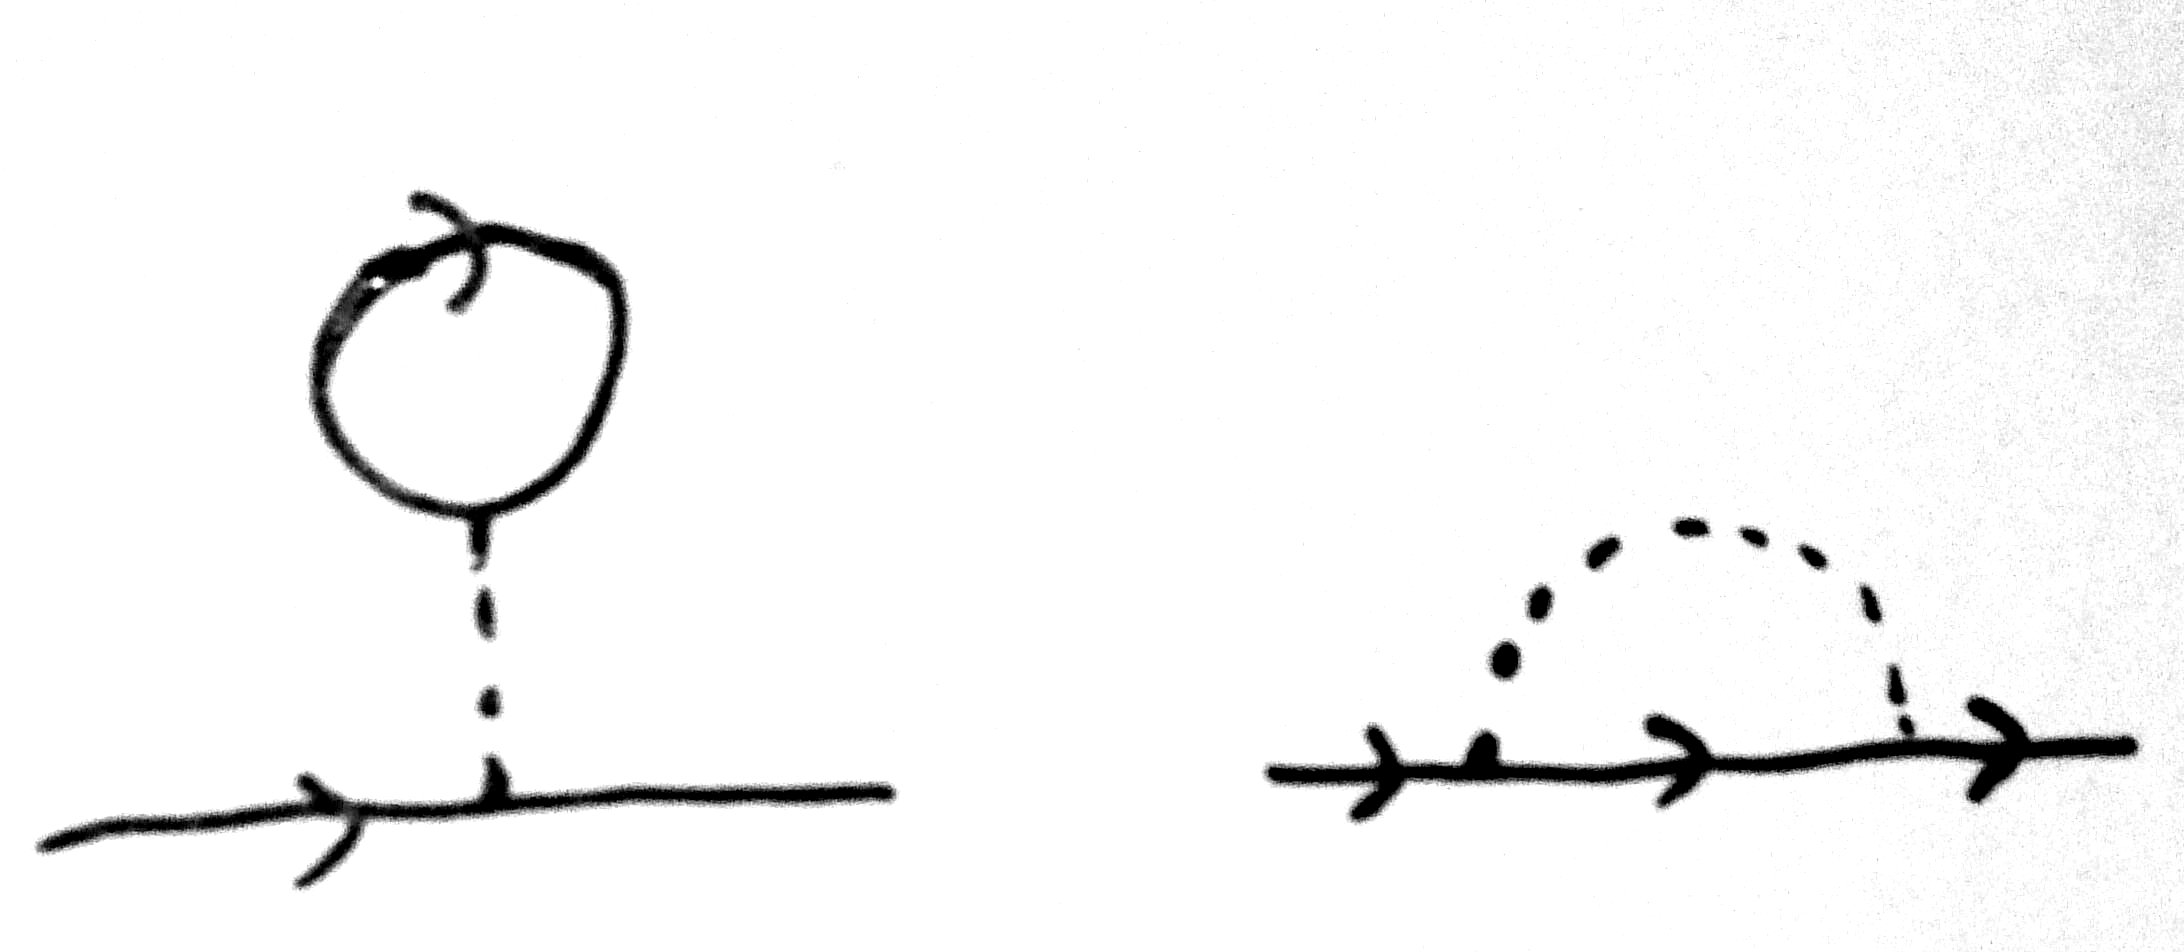
\includegraphics[width=10cm]{Zero/1stFDiagram.jpg}
\caption{一阶连接图}
%\label{default}
\end{center}
\end{figure}

\item

引入连接图和非连接图概念后,格林函数可表示为:

\begin{equation}
iG = \frac{\left\langle \Phi_0 \right| T ( \psi \psi^\dagger S ) \left| \Phi_0  \right\rangle_c \times \left\langle \Phi_0 \right|  S  \left| \Phi_0 \right\rangle_{nc}}{ \left\langle \Phi_0 \right|  S  \left| \Phi_0 \right\rangle_{nc}} = \left\langle \Phi_0 \right| T ( \psi \psi^\dagger S ) \left| \Phi_0 \right\rangle_c
\end{equation}

即格林函数可表示为所有拓扑不等价的连接图形之和!

\begin{figure}[htbp]
\begin{center}
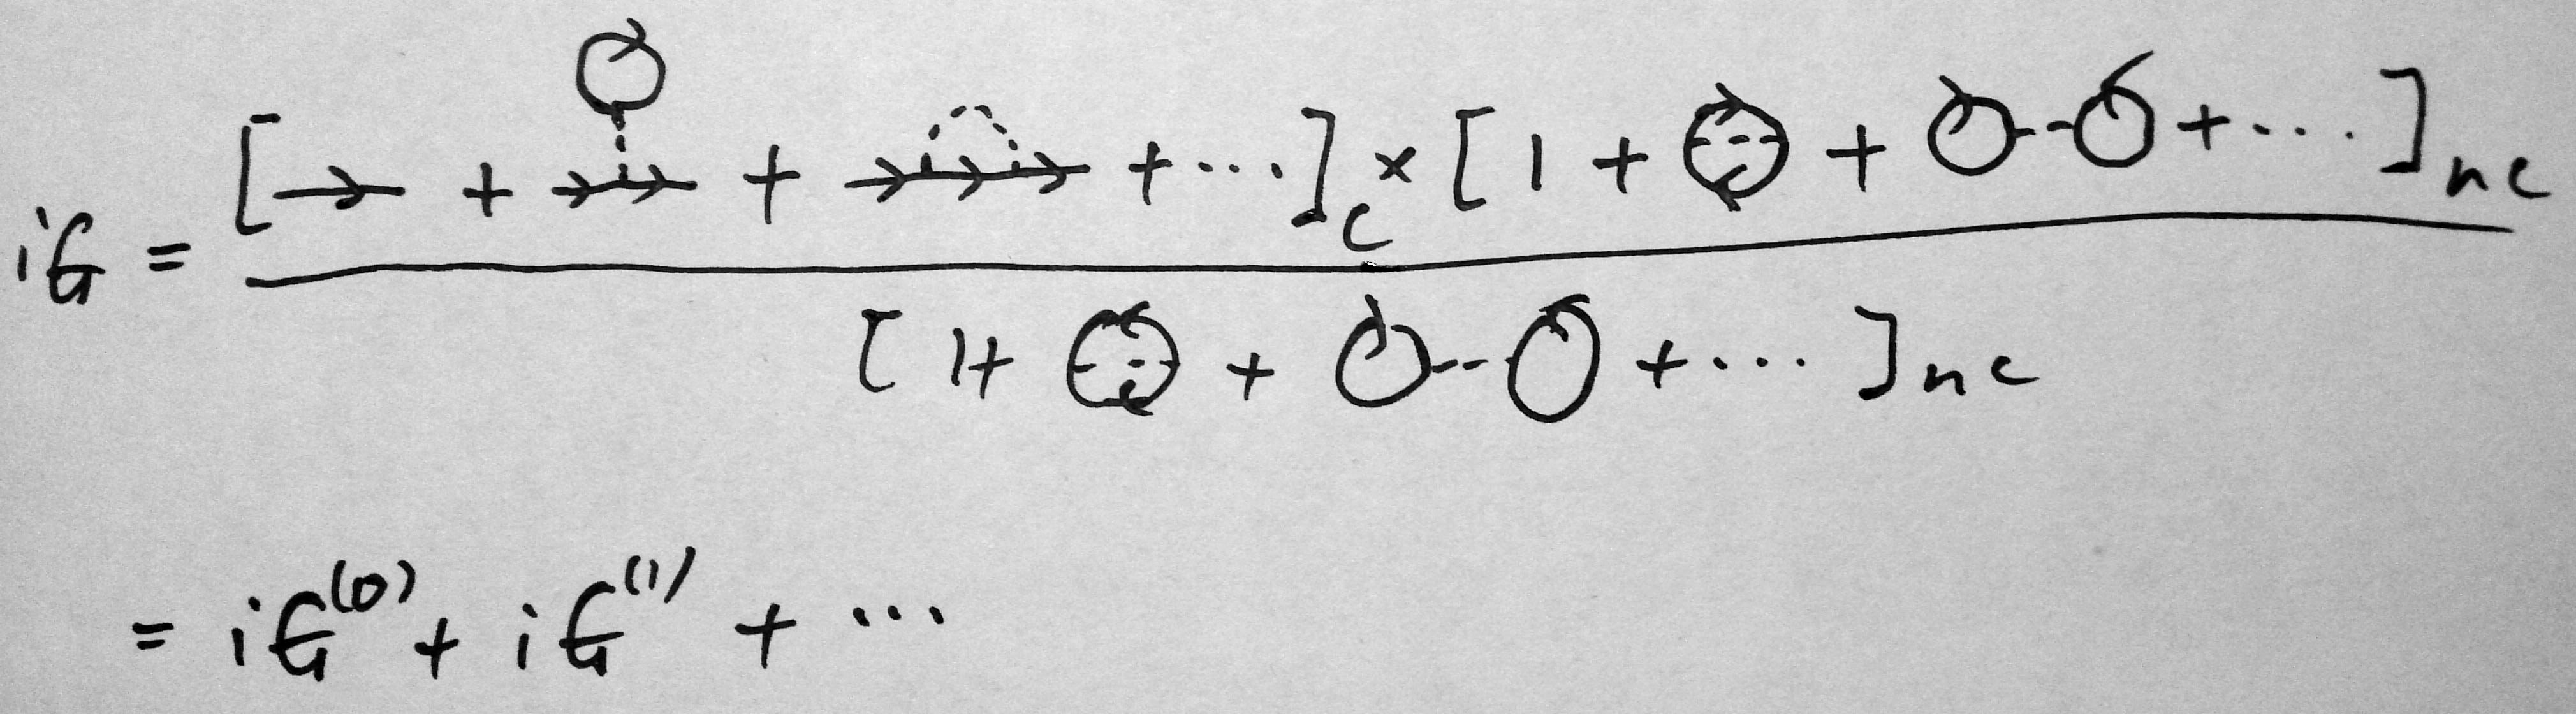
\includegraphics[width=11cm]{Zero/FDconnected.jpg}
\caption{非连接图形的部分正好被消掉了。}
%\label{default}
\end{center}
\end{figure}

\item

对从一点出发又回到这一点的单粒子线,或连接在相同相互作用线上的粒子线,时间宗量相同,此时我们必须规定:T乘积内$\psi^\dagger$的时间要比$\psi$的大一个无限小量$\eta$。

\begin{equation}
i G^0 (x , x) = \left\langle \Phi_0 \right|  T (\psi(x,t) \psi^\dagger (x,t+\eta) ) \left| \Phi_0 \right\rangle = iG^0 (-\eta)
\end{equation}

同时,

\begin{equation}
i G^0 (x , x) = - \left\langle \Phi_0 \right| \psi^\dagger  \psi   \left| \Phi_0 \right\rangle = - n^0 (x)
\end{equation}

\item 

一个闭合粒子线对应一个“-”,相当于有一个传播子是从未来传回来的。在$G^{(n)}$中如果有$F$个闭合粒子线,则有因子$(-1)^F$。

\end{enumerate}


\subsection{动量空间的图形规则}


\begin{enumerate}

\item 

\begin{eqnarray*}
G(x,y) & = & (2 \pi)^{-4} \int d^4 k  e^{i k \cdot (x-y)} G(k) \\
U(x, x') & = & (2 \pi)^{-4} \int d^4 k e^{i k \cdot (x-x')} U(k) \\
\end{eqnarray*}

这里$d^4 k \to d^3 k d \omega$, $k \cdot x \to k \cdot x - \omega t $

\item

对每个内定点,动量、能量守恒:

\begin{equation}
\delta^{(4)} (q - q' + q'') = (2 \pi)^{-4} \int d^4 x e^{i (q- q' + q'') \cdot x}
\end{equation}

\item

对$G(k,\omega)$的第n级贡献$G^{(n)} (k, \omega)$,

首先画出n根相互作用线,和$2n + 1$根有向粒子线的所有拓扑不等价的连接图形。

\item

对每个内定点要求动量-能量守恒,总共有$2n$个守恒条件。

\item 

对内线的自旋指标求和。

对$n$个独立的内部四维动量(哑元)积分。

(总共有$3n + 1$个粒子线或相互作用线,去掉$2n$个守恒条件,再去掉1个外线,还剩$n$个独立的内线。)

\item

每一项附加因子

\begin{equation*}
i^n (2 \pi)^{-4n} (-1)^F
\end{equation*}

这里$F$是闭合费米子线的个数。

\item

对每个形成闭合环的单粒子线,或与同一根相互作用线相连的单粒子线。

对$G(- \eta)$做傅里叶变换,为:$e^{i \omega \eta} G(k, \omega)$

\end{enumerate}

作为练习,我们可计算动量空间中的一阶图形。

\begin{eqnarray*}
G^{(1)} & = & G^{(1)}_a + G^{(1)}_b \\
G^{(1)}_a & = & i G^0 (k) (2 \pi)^{-4} \int d^4 p V(k-p) G^0 (p) G^0 (k)  \\
G^{(1)}_b & = & i (-1) G^0 (k) (2 \pi)^{-4} \int d^4 p G^0 (p) V(0) G^0 (k)
\end{eqnarray*}

这里:$G^0 (p) \to e^{i \omega \eta}  G(p, \omega)  $




\section{戴逊级数}

\subsection{自能}

有了图形表示后,重要的是对图形进行分类。可以使用各种各样的标准对图形进行分类。比如按考虑相互作用的阶数进行分类:

\begin{eqnarray*}
i G (x,x') & = & \left\langle \Phi_0 \right| T \left( \psi(x) \psi^\dagger (x') S \right) \left| \Phi_0  \right\rangle_c \\
{} & = & i G^{(0)} + iG^{(1)} + iG^{(2)} + ... 
\end{eqnarray*}

对$i G^{(1)}$,有两个图:

\begin{equation*}
G^{(1)}(k) = G_a^{(1)} (k) + G_b^{(1)} (k) = G^{(0)}(k) \Sigma^{(1)}(k) G^{(0)}(k)
\end{equation*}

这里的$\Sigma^{(1)}(k)$叫一阶自能:

\begin{equation}
\Sigma^{(1)}(k) = \frac{i}{(2 \pi)^4 } \int d^4p e^{i p_0 \eta} \left( V(k-p) G^{(0)}(p)  - V(0) G^{(0)}(p)  \right) 
\end{equation}

按照这个思路还可以考虑二阶自能$\Sigma^{(2)}(k) $,即包含两根相互作用线的自能图。

对二阶自能图,可分成两类,一类是切断一根单粒子线,自能图就能分成独立的两部分,每一部分分别是个一阶自能图:

\begin{equation*}
\Sigma^{(1)} G^{(0)}  \Sigma^{(1)}
\end{equation*}

还有一类,是不能通过切断一根单粒子线分成不相连两部分的。这部分是真正不同于一阶图形的部分,我们称之为正规自能。当然这里是二阶的正规自能$\Sigma^{(2)*}$。

我们可以把各阶的正规自能都加在一起,得到作为整体的正规自能$\Sigma^*$。

\begin{equation}
\Sigma^* = \Sigma^{(1)*} + \Sigma^{(2)*} + ...
\end{equation}

自能$\Sigma$可表示为:

\begin{equation}
\Sigma = \Sigma^* + \Sigma^* G^{(0)} \Sigma^* + \Sigma^* G^{(0)} \Sigma^* G^{(0)} \Sigma^* + ...
\end{equation}

这是一种对图形的分类,即正规自能,通过一根单粒子线连接起的两个正规自能,通过两根单粒子线连接起的三个正规自能……,这种分类方式并不遗漏,也不重复。

将格林函数用自能$\Sigma (k)$表示,

\begin{equation}
G(k) = G^{(0)}(k) + G^{(0)}(k) \Sigma(k) G^{(0)}(k)
\end{equation}

将格林函数用正规自能$\Sigma^* (k)$表示,

\begin{equation}
G(k) = G^{(0)}(k) + G^{(0)}(k) \Sigma^* (k) G(k)
\end{equation}

把$G(k)$都挪到左边:

\begin{equation*}
G(k) \left( 1 - G^{(0)} (k) \Sigma^* (k)  \right) = G^{(0)}(k)  
\end{equation*}

注意:这里的$G$,$G^0$,$\Sigma^* $都是$c$数,

\begin{equation*}
G^{-1} = \left( G^{(0)} \right)^{-1} \left( 1 - \Sigma^*  G^{(0)}  \right) = \left( G^{(0)} \right)^{-1} - \Sigma^*
\end{equation*}

这意味着:

\begin{equation}
G(k) = \frac{1}{  \left( G^{(0)} (k) \right)^{-1} - \Sigma^* (k)  }
\end{equation}

正规自能的实部是对准粒子能量的修正,而正规自能的虚部是对准粒子寿命的修正。考虑相互作用后格林函数的求解被归结为对正规自能的求解。

\subsection{一阶自能}

作为例子,我们来计算$\Sigma^{(1)}(k)$,先计算积分:

\begin{equation}
\frac{-i}{(2 \pi)^4} \int d^4 p V(0) G^{(0)}(p) e^{i p_0 \eta}
\end{equation}

改写为:

\begin{equation*}
-i \int \frac{d^3 p}{(2 \pi)^3} \int \frac{ d \omega }{ 2 \pi } V(0) \left( \frac{\theta(p - p_F)}{ \omega - \epsilon_p + i \eta } + \frac{ \theta(p_F - p) }{ \omega - \epsilon_p - i \eta }    \right) e^{i \omega \eta}
\end{equation*}

对$e^{i \omega \eta}$,积分回路取上半平面,沿大圆的积分为0。

\begin{equation*}
\oint ... = \int_{- \infty}^{\infty} ... = 2 \pi i (Rez (\omega = \epsilon_p + i \eta)) = 2 \pi i \frac{ \theta(p_F - p) }{2 \pi} = i \theta(p_F - p)
\end{equation*}

考虑:$\int d^3 x \int \frac{d^3 p}{(2 \pi)^3} ... = V \int \frac{d^3 p}{(2 \pi)^3} ... = N $

\begin{equation*}
-i \int \frac{d^3 p}{(2 \pi)^3} ... = - i \cdot i \frac{N}{V} V(0)= n V(0) 
\end{equation*}

类似地,计算积分,

\begin{equation*}
i \int \frac{d^3 p}{(2 \pi)^3 } \int \frac{ d \omega }{ 2 \pi } e^{i \omega \eta } V(k-p) \left(  \frac{\theta(p-p_F)}{ \omega - \epsilon_p + i \eta}  + \frac{ \theta(p_F -p)  }{ \omega - \epsilon_p - i \eta }     \right)
\end{equation*}

先利用留数定理对$\omega$积分,

\begin{equation*}
 - \int \frac{d^3 p}{(2 \pi)^3 } V(k-p) \theta(p_F - p)
\end{equation*}

得到$\Sigma^{(1)}(k)$的表达式:

\begin{equation}
\Sigma^{(1)}(k) = n V(0) - \frac{1}{(2 \pi)^3} \int d^3 p V ( \vec k - \vec p ) \theta( p_F - | \vec p | )
\end{equation}

考虑$\Sigma^{(1)}(k)$的近似是超出普通的微扰论的,因为在公式$G^{-1} = \left( G^{(0)} \right)^{-1} - \Sigma^* $里已经考虑了很多诸如$\Sigma^1 G^0 \Sigma^1$,$\Sigma^1 G^0 \Sigma^1 G^0 \Sigma^1$...的近似。

\subsection{极化}

\begin{equation*}
U(q) = V(q)  + V(q) \Pi(q) V(q)
\end{equation*}

这里$V$表示裸相互作用线,$U$表示考虑了多体效应后的相互作用线。我们称$\Pi(q) $为极化。

\begin{figure}[htbp]
\begin{center}
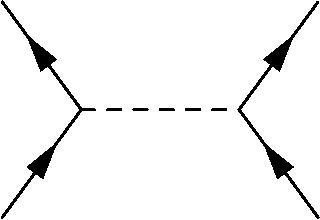
\includegraphics[width=5cm]{Zero/polarized.png}
\caption{裸相互作用线,我们可以在裸相互作用线里不断插入“泡泡”图。}
%\label{default}
\end{center}
\end{figure}

类似于自能,我们把极化分为两类,正规极化$\Pi^*$,和非正规极化$\Pi_{ir}$,正规极化是无法通过切断一根裸相互作用线而把极化分为两个不连接的两部分的极化图形。

极化$\Pi$可以用正规极化$\Pi^*$来表示:

\begin{equation}
\Pi = \Pi^* + \Pi^* V \Pi^* + \Pi^* V \Pi^* V \Pi^* + ... 
\end{equation}

考虑极化后的相互作用线$U$,可以用正规极化$\Pi^*$来表示:

\begin{equation}
U = V + V \Pi^* U
\end{equation}

或改写为:

\begin{equation*}
U (1 - \Pi^* V) = V
\end{equation*}

即:

\begin{eqnarray*}
U(q)  & = &  \frac{V(q)}{1 - \Pi^*(q) V(q) } = \frac{V(q)}{\epsilon(q)} \\
{} & = & V(q) ( 1 + \Pi^* (q) V (q) + \Pi^* (q) V (q) \Pi^* (q) V (q) + ...  )
\end{eqnarray*}

这里:$\epsilon(q) = 1 - \Pi^*(q) V(q) $


\chapter{有限温度}

\section{松原函数}

\subsection{热力学格林函数}

零温格林函数被定义为:

\begin{equation}
i G(1,2) = \left\langle 0 \right| T ( \psi(1) \psi^\dagger (2)) \left| 0 \right\rangle
\end{equation}

有限温度,系统将可出于激发态$\left| n \right\rangle$,定义激发态的单粒子格林函数为:

\begin{equation}
i G (1,2: n) =  \left\langle n \right| T ( \psi(1) \psi^\dagger (2)) \left| n \right\rangle
\end{equation}

系统出于激发态$\left| n \right\rangle$的几率是$e^{- \beta ( E_n - \mu N )}$,对$i G(1,2: n)$求统计平均,

\begin{equation}
i G(1,2: \beta, \mu) = Tr \left[ \rho_G T( \psi(1) \psi^\dagger(2) ) \right] = \sum\limits_{N, n} e^{\beta \Omega} e^{- \beta ( E_n - \mu N )} \left\langle n \right|  T (\psi(1) \psi^\dagger (2)) \left| n \right\rangle   
\end{equation}

这里$e^{\beta \Omega}$ 是归一化常数,

\begin{equation}
e^{-\beta \Omega} = Tr e^{- \beta (H - \mu N)}
= \sum\limits_{N,n} e^{-\beta (E_n - \mu N)}
\end{equation}

\subsection{虚时变换}


回忆海森堡绘景的变换关系:

\begin{equation}
O_H (t) = e^{i H t} O e^{- i H t}
\end{equation}

这里我们使用$K = H - \mu N$替代$H$

\begin{eqnarray*}
\psi (t) = e^{i K t}  \psi e^{-i K t}  \\
\psi^\dagger (t) = e^{i K t } \psi^\dagger e^{- i Kt}
\end{eqnarray*}

对$t_1 > t_2$,

\begin{eqnarray*}
i G(1,2) & = & Tr \left[  e^{\beta \Omega} e^{ - \beta K }  e^{i K t_1} \psi(x_1) e^{-i K t_1} e^{ i K t_2} \psi^\dagger (x_2) e^{- i K t_2}   \right] \\
{} & = & Tr \left[  e^{\beta \Omega} e^{ - \beta K }  e^{i K ( t_1 - t_2 )} \psi(x_1) e^{-i K (t_1 -t_2)} \psi^\dagger (x_2)   \right]
\end{eqnarray*}

对$t_1 < t_2$,

\begin{eqnarray*}
i G(1,2) & = & \mp  Tr \left[  e^{\beta \Omega} e^{ - \beta K }  e^{i K t_2} \psi^\dagger(x_2) e^{-i K t_2} e^{ i K t_1} \psi (x_1) e^{- i K t_1}  \right] \\
{} & = & \mp Tr \left[  e^{\beta \Omega} e^{ - \beta K }  e^{- i K ( t_1 - t_2 )} \psi^\dagger(x_2) e^{ i K (t_1 -t_2)} \psi (x_1)   \right]
\end{eqnarray*}

由$e^{i H t}$ 和$e^{- \beta H}$的相似性,构造$ it \to \tau $的变换。

定义松原函数$\mathcal{ G } (1,2)$, 当$\tau_1 > \tau_2$时:

\begin{equation*}
\mathcal{ G } (1,2) = - Tr \left[ e^{\beta \Omega} e^{-\beta K}  e^{K(\tau_1 - \tau_2)} \psi(1) e^{- K(\tau_1 - \tau_2)} \psi^\dagger (2)   \right] 
\end{equation*}

$\tau_1 < \tau_2$时,


\begin{equation*}
\mathcal{ G } (1,2) = \pm Tr \left[ e^{\beta \Omega} e^{-\beta K}  e^{- K(\tau_1 - \tau_2)} \psi^\dagger (2) e^{ K(\tau_1 - \tau_2)} \psi(1)   \right] 
\end{equation*}

\subsection{松原函数的一个性质}

利用松原函数的定义,我们可以证明:

\begin{equation}
\mathcal{G} (\tau < 0) =  \mp \mathcal{ G } (\tau + \beta > 0)
\end{equation}

对费米子取“-”,对波色子取“+”。$\tau \in [-\beta , \beta ]$,定义傅里叶变换:

\begin{eqnarray*}
\mathcal{G} (\tau) &=& \frac{1}{\beta} \sum\limits_n e^{-i \omega_n \tau} \mathcal{G} (i \omega_n) \\
\mathcal{G} (i \omega_n) & = & \frac{1}{2} \int_{- \beta}^{\beta} d \tau e^{i \omega_n \tau} \mathcal{G} (\tau) 
\end{eqnarray*}

这里要求$2 \beta \omega_n = 2 n \pi $,即:$\omega_n = \frac{n \pi}{\beta}$

利用$\mathcal{G} (\tau < 0)  = \mp \mathcal{G}(\tau + \beta >0) $,计算$\mathcal{G} (i \omega_n)$,

\begin{eqnarray*}
\mathcal{G} (i \omega_n) & = & \int_{-\beta}^0 d \tau e^{i \omega_n \tau } \mathcal{G} ( \tau ) + \frac{1}{2} \int_0^\beta d \tau e^{i \omega_n \tau } \mathcal{G} ( \tau ) \\
{} & = & \frac{1}{2} (1 \mp e^{-i \omega_n \beta} ) \int_0^\beta d \tau e^{i \omega_n \tau} \mathcal{G}(\tau)
\end{eqnarray*}

讨论因子$\frac{1}{2} (1 \mp e^{-i \omega_n \beta} )$,对费米子,当$n$取奇数时,为1。对玻色子,当$n$取偶数时,为1。其他情况都是0。

\subsection{无相互作用系统的松原函数}

考虑无相互作用的费米子系统,哈密顿量可写为:

\begin{equation}
K_0 = H_0 - \mu N = \sum\limits_{k} ( \epsilon_k - \mu ) a_k^\dagger a_k
\end{equation}

定义傅里叶变换:

\begin{eqnarray*}
\psi(x)  &=& V^{-1/2} \sum\limits_k e^{i k x} a_k  \\
\psi^\dagger (x)  &=& V^{-1/2} \sum\limits_k e^{- i k x} a^\dagger_k 
\end{eqnarray*}

对费米子,每个态$k$(这里先不考虑自旋指标,或把自旋归于指标$k$),或者占据0个费米子,或者占据1个费米子。对$\left| 0 \right\rangle$和$\left| 1 \right\rangle$我们都可证明:

\begin{eqnarray*}
e^{K_0 \tau} a_k e^{- K_0 \tau} &=& a_k e^{ -(\epsilon_k - \mu)\tau } \\
e^{K_0 \tau} a^\dagger_k e^{- K_0 \tau} &=& a^\dagger_k e^{ (\epsilon_k - \mu) \tau}
\end{eqnarray*}

海森堡绘景下的$\psi$, 和$\psi^\dagger$

\begin{eqnarray*}
\psi(x,\tau) &=& e^{K_0 \tau} \psi(x) e^{-K_0 \tau} = V^{-1/2} \sum\limits_k e^{ikx} e^{ -(\epsilon_k - \mu)\tau } a_k\\
\psi^\dagger (x,\tau) &=& e^{K_0 \tau} \psi^\dagger (x) e^{-K_0 \tau} = V^{-1/2} \sum\limits_k e^{- ikx} e^{ (\epsilon_k - \mu)\tau } a^\dagger_k
\end{eqnarray*}

现在来计算无相互作用时松原函数$\mathcal{G}^0$,

\begin{equation}
\mathcal{G}^0(1,2)=- e^{\beta \Omega_0} Tr \left( e^{-\beta K_0} T [ \psi(1) \psi^\dagger (2) ] \right)
\end{equation}

假设$\tau_1 > \tau_2$

\begin{equation*}
\mathcal{G}^0(1,2) = - V^{-1} \sum\limits_{k k'} ... \left\langle a_k a^\dagger_{k'}  \right\rangle
\end{equation*}

这里:

\begin{equation}
\left\langle a_k a^\dagger_{k'}  \right\rangle = \delta_{kk'} (1 \mp n_k^0)
\end{equation}

于是对$k$的求和变成是一重的了。

\begin{equation}
\mathcal{G}^0 (1,2) = - V^{-1} \sum\limits_k e^{i k (x_1 - x_2) - (\epsilon_k - \mu) (\tau_1 - \tau_2) }  (1 \mp n_k^0)
\end{equation}

这里:

\begin{equation*}
V^{-1} \sum\limits_k \to \frac{1}{(2 \pi)^3} \int d^3 k
\end{equation*}

定义傅里叶变换:

\begin{equation}
\mathcal{G}^0 (x, \tau) = \mathcal{G}^0 (1,2) = \frac{1}{(2\pi)^3} \int d^3 k  e^{i k x} \frac{1}{\beta} \sum\limits_n e^{-i \omega_n \tau} \mathcal{G}^0 (k, i\omega_n)
\end{equation}

逆傅里叶变换:

\begin{equation}
\mathcal{G}^0 (k, i\omega_n) = \int_0^\beta d \tau e^{i \omega_n \tau} \int d^3 x e^{-i k x} \mathcal{G}^0 (x, \tau) 
\end{equation}

把$\mathcal{G}^0(x, \tau)$的表达代入上式:

\begin{equation*}
\mathcal{G}^0 (k, i\omega_n)  = \int_0^\beta d \tau e^{i \omega_n \tau} \int d^3 x e^{-i k x} \left( -\frac{1}{(2 \pi)^3 } \right)  \int d^3 k' e^{i k' x } e^{- (\epsilon_{k'} - \mu) \tau} (1 \mp n_{k'}^0)
\end{equation*}

在上式积分中先计算$\int d^3 x e^{-i(k-k')x} = \delta(k-k')$,然后再计算$\frac{1}{(2 \pi)^3}  \int d^3 k' \delta( k - k')... = ...$。最后只剩下对$d \tau$的积分:

\begin{equation*}
\mathcal{G}^0 (k, i \omega_n) = - \int_0^\beta d \tau e^{i \omega_n \tau} e^{-(\epsilon_k - \mu)\tau }(1 \mp n_k^0)
\end{equation*}

对费米子,$\omega_n = \frac{(2n +1 )\pi}{\beta}$,$n_k^0 = \frac{1}{e^{\beta (\epsilon - \mu)} + 1}$,

\begin{equation}
\mathcal{G}^0 (k, i \omega_n) = \frac{1}{i \omega_n - \epsilon_k + \mu}
\end{equation}


\subsection*{练习}

自由声子场的哈密顿量是:

\begin{equation}
H_0 = \sum\limits_k \omega_0 (k) \left( b^\dagger_k b_k + \frac{1}{2} \right)
\end{equation}


证明自由声子的松原函数$\mathcal{D}^0(k, \omega_n)$可表示为:

\begin{equation}
\mathcal{D}^0 (k, \omega_n) = \frac{1}{i \omega_n - \omega_0(k)} - \frac{1}{i \omega_n + \omega_0(k)} = - \frac{2 \omega_0 (k)}{  \omega_n^2 + \omega_0^2(k)  }
\end{equation}

这里$\omega_n = \frac{2 n \pi}{\beta}$。

\section{有限温度下的微扰论}

\subsection{推广的相互作用绘景}

推广的海森堡绘景下,算符可表示为($\hbar = 1$):

\begin{equation*}
O_K (\tau) = e^{K \tau} O_S e^{-K \tau}
\end{equation*}

这里: $K = H - \mu N$.


推广的相互作用绘景:

\begin{equation*}
O_I (\tau ) = e^{K_0 \tau} O_S e^{-K_0 \tau}
\end{equation*}

这里: $K_0 = H_0 - \mu N$, $K- K_0 = H - H_0 = H'$,
我们亦可用$O_I$来表示$O_S$,

\begin{equation*}
O_S = e^{-K_0 \tau} O_I (\tau) e^{K_0 \tau}
\end{equation*}

得到$O_K (\tau)$与$O_I (\tau)$之间的关系,

\begin{equation}\label{OK-OI-relation}
O_K(\tau) = e^{K \tau} e^{-K_0 \tau} O_I (\tau) e^{K_0 \tau}
e^{-K\tau}
\end{equation}

定义相互作用绘景下的演化算符为:

\begin{equation*}
U(\tau_1, \tau_2) = e^{K_0 \tau_1} e^{-K(\tau_1 - \tau_2)} e^{-K_0
\tau_2}
\end{equation*}

关系(\ref{OK-OI-relation})可改写为:

\begin{equation*}
O_K (\tau) = U(0, \tau) O_I (\tau) U(\tau, 0)
\end{equation*}

这里,

\begin{eqnarray*}
% \nonumber to remove numbering (before each equation)
  U(0,\tau) &=& e^{K\tau}e^{-K_0\tau} \\
  U(\tau,0) &=& e^{K_0 \tau} e^{-K\tau}
\end{eqnarray*}

必须指出的是$U$不是幺正算符, 即不满足$U^\dagger U =1$,
但$U$满足以下性质:

\begin{eqnarray*}
% \nonumber to remove numbering (before each equation)
  U(\tau_1, \tau_2) U(\tau_2, \tau_3) &=& U(\tau_1, \tau_3) \\
  U(\tau_1, \tau_1) &=& 1 \\
  U(\tau, 0)U(0, \tau) &=& U(0, \tau) U(\tau, 0) =  1
\end{eqnarray*}

推广的相互作用绘景下, 可求对$U$的偏导, $\frac{\partial U}{\partial
\tau}$,

\begin{equation}\label{time-evolution-of-U-tau}
\frac{\partial }{\partial \tau} U (\tau, 0) = - H'_I (\tau) U(\tau,
0)
\end{equation}

一阶微分方程, 存在形式解:

\begin{equation*}
U(\tau, 0) = 1 - \int_0^\tau d\tau_1 H'_I (\tau_1) U(\tau_1,0)
\end{equation*}

等式左右都有$U$, 反复迭代得到:

\begin{equation}\label{dyson-series-at-ft}
U(\tau,0) = \sum_{n=0}^\infty \frac{(-1)^n}{n!} \int_0^\tau d\tau_1
...\int_0^\tau d\tau_n T_\tau \left[ H'_I(\tau_1)...H'_I (\tau_n)
\right]
\end{equation}

考虑配分函数$e^{-\beta \Omega}$,

\begin{equation*}
e^{-\beta \Omega} = Tr e^{-\beta K} = Tr e^{-\beta K_0} e^{\beta
K_0} e^{-\beta K} = Tr \left[ e^{-\beta K_0} U(\beta , 0) \right]
\end{equation*}

利用迭代展开(\ref{dyson-series-at-ft}), 上式化为:

\begin{equation*}
e^{-\beta \Omega} = \sum_{n=0}^{\infty} \frac{(-1)^n}{n!}
\int_0^\beta d\tau_1 ... \int_0^\beta d\tau_n Tr \left[ e^{-\beta
K_0} T_\tau \left( H'_I(\tau_1)...H'_I(\tau_n) \right) \right]
\end{equation*}

回忆松原函数的定义, 仅写出$\tau > \tau'$的情形,

\begin{eqnarray*}
% \nonumber to remove numbering (before each equation)
  \mathcal{ G }_{\alpha, \beta}(x\tau,x'\tau') &=& - Tr \left\{e^{\beta(\Omega - K)} \psi_{K\alpha}(x\tau) \psi_{K\beta}^\dagger(x'\tau') \right\} \\
  {} &=& - e^{\beta \Omega} Tr \left\{ e^{-\beta K} \psi \psi^\dagger \right\} \\
  {} &=& - e^{\beta \Omega} Tr \left\{ e^{-\beta K_0} e^{\beta K_0} e^{-\beta K} ...
  \right\} \\
  {} &=& - e^{\beta \Omega} Tr \left\{ e^{-\beta K_0} U(\beta, 0) ...
  \right\}
\end{eqnarray*}

这里, $... = U(0,\tau) \psi_{I\alpha}(x\tau)U(\tau,0)U(0,\tau')
\psi_{I\beta}^\dagger(x'\tau') U(\tau',0)$.

因此,

\begin{equation*}
\mathcal{ G }_{\alpha\beta}(x\tau,x'\tau') = - \frac{ Tr \left\{
 e^{-\beta K_0} U(\beta,\tau) \psi_{I \alpha}(x \tau) U (\tau,\tau') \psi_{I \beta}^\dagger (x'\tau')U(\tau',0)  \right\} }{Tr \left\{ e^{-\beta K_0} U(\beta,0) \right\} }
\end{equation*}

即:

\begin{equation*}
\mathcal{ G }_{\alpha\beta}(x\tau,x'\tau') = - \frac{ Tr \left\{
 e^{-\beta K_0} T_\tau \left[ \psi_{I \alpha}(x \tau) \psi_{I \beta}^\dagger (x'\tau') U(\beta,0) \right] \right\} }{Tr \left\{ e^{-\beta K_0} U(\beta,0) \right\} }
\end{equation*}


引入记号$\left\langle ... \right\rangle_0 = Tr \left\{ e^{\beta
\Omega_0} e^{-\beta K_0} ... \right\}$,
即表示对无相互作用系统求热力学平均。


最终, 松原函数可写为:

\begin{equation*}
\mathcal{ G }_{\alpha\beta}(x\tau,x'\tau') = - \frac{\left\langle
T_\tau \left\{ \psi_{I\alpha}(x\tau)\psi_{I\beta}^\dagger (x'\tau')
U(\beta,0) \right\} \right\rangle_0  }{ \left\langle U(\beta, 0)
\right\rangle_0 }
\end{equation*}


\subsection{有限温度的维克定理}

类似于零温时的维克定理, 我们有:

\begin{equation}\label{wick th at ft}
\left\langle T_\tau (ABCD...) \right\rangle_0 = \sum_P (\mp)^P
\left\langle T_\tau(AB) \right\rangle_0 \left\langle T_\tau(CD)
\right\rangle_0 ...
\end{equation}


这里$P$表示的是所有``配对''方式,
$(\mp)^P$是不同算符``配对''引入的因子, 只对费米子有意义。
与零温时维克定理的区别是, 这里的$\left\langle ...
\right\rangle_0$是对无相互作用系统求的热力学平均,
而前者是对无相互作用系统求的基态(量子力学)平均。

我们可证明,

\begin{eqnarray*}
% \nonumber to remove numbering (before each equation)
  \left\langle T_\tau (\psi_{I\alpha}(x\tau) \psi_{I\beta}^\dagger (x'\tau')) \right\rangle_0 &=& - \mathcal{ G }_{\alpha \beta}^0 (x\tau, x'\tau') \\
  \left\langle T_\tau (\psi \psi) \right\rangle_0 &=& 0 \\
  \left\langle T_\tau (\psi^\dagger \psi^\dagger) \right\rangle_0 &=&
  0
\end{eqnarray*}


\subsection{有限温度的费曼图}

类似零温格林函数的讨论, 我们只需考虑连接图形:

\begin{equation*}
\mathcal{G}_{\alpha \beta}(x\tau,x'\tau') = - \left\langle T_\tau
\left\{ \psi_{I\alpha}(x\tau)\psi_{I\beta}^\dagger(x'\tau')
U(\beta,0) \right\} \right\rangle_c
\end{equation*}

...

回忆松原函数的傅立叶变换和逆傅立叶变换,

\begin{eqnarray*}
% \nonumber to remove numbering (before each equation)
  \mathcal{G}_{\alpha \beta}(x\tau) &=& \frac{1}{\beta} \sum_n \frac{1}{(2\pi)^3}\int d^3 p e^{ipx-i\omega_n \tau} \mathcal{G}_{\alpha \beta}(p,i\omega_n) \\
  \mathcal{G}_{\alpha \beta} (p,i\omega_n) &=& \int_0^\beta d \tau \int d^3 x  e^{-ipx + i \omega_n \tau} \mathcal{G}_{\alpha \beta} (x\tau)
\end{eqnarray*}

这里,

\begin{eqnarray*}
% \nonumber to remove numbering (before each equation)
  \omega_n &=& \frac{(2n+1)\pi}{\beta}, Fermions \\
  \omega_n &=& \frac{2n\pi}{\beta}, Bosons
\end{eqnarray*}

对无相互作用费米子, 我们曾经求得:

\begin{equation*}
\mathcal{G}_{\alpha \beta}^0 (p, i\omega_n) = \frac{\delta_{\alpha
\beta }}{i \omega_n - \epsilon_p^0 + \mu}
\end{equation*}

考虑相互作用:

\begin{equation}
V(x, \tau) = V(x_1 - x'_1)\delta(\tau_1 - \tau'_1) = \frac{1}{\beta} \sum\limits_n \frac{1}{(2\pi)^3}\int d^3 q e^{i (q x - \omega_n \tau)} V(q, \omega_n)
\end{equation}

这里:

\begin{equation}
\delta (\tau) = \frac{1}{\beta} \sum\limits_n e^{i \omega_n \tau} 
\end{equation}

(证明的思路是这样的:(1)当$\tau \neq 0$时,$\frac{1}{\beta} \sum\limits_n ... = 0 $;(2)当$\tau \to 0 $,$\frac{1}{\beta} \sum\limits_n ... \to \infty $;(3)积分:$ \frac{1}{\beta}  \int_0^{\beta}  d \tau (1 + e^{i \omega_1 \tau} +  e^{i \omega_2 \tau} + ... ) = 1 + 0 = 1 $。)

$\omega_n = \frac{2n \pi}{\beta}$, 导致:$V(q, \omega_n) = V(q)$,

\begin{eqnarray}
V(x)  &=&  \frac{1}{(2\pi)^3} \int d^3 q e^{i q x} V(q) \\
V(q) &=& \int d^3 x e^{-i q x} V(x)
\end{eqnarray}

对实空间画出费曼图,然后再做FT,对每一个内顶点都有能量-动量守恒。

\begin{equation}
\frac{1}{\beta} \int_0^{\beta} d \tau e^{i (\omega_n'' - \omega_n - \omega_n') \tau } = \delta_{\omega_n'' - \omega_n - \omega_n'}
\end{equation}

这里:$\omega_n$, $\omega_n''$ 是粒子线,$n$, $n''$可能取奇数,也可能取偶数,但其差一定取偶数。

$\omega_n'$ 是相互作用线,$n'$取偶数。

\subsubsection{动量空间的图形法则}

计算$\mathcal{G} (p, i \omega_n)$第n级贡献的费曼图形法则:

\begin{enumerate}
\item

画出n条相互作用线,2n+1条有向粒子线所有拓扑不等价连接图形。

为每一根相互作用线指定一个方向,并与一个波矢和分立的频率相联系。波矢和频率在每一个顶点上守恒。

\item

对费米子而言,$\omega_n = \frac{(2n +1)\pi}{ \beta}$。

\begin{equation*}
\mathcal{G}_{\alpha \beta}^0 (p, i\omega_n) = \frac{\delta_{\alpha
\beta }}{i \omega_n - \epsilon_p^0 + \mu}
\end{equation*}


对玻色子而言,$\omega_n = \frac{2n\pi}{ \beta}$。
 
\item

相互作用线振幅:$V(k, \omega_n) = V(k)$

\item

对所有独立的n个内波矢积分,对所有独立的n个内频率求和。

\begin{equation*}
\frac{1}{\beta} \sum\limits_n \frac{1}{(2 \pi)^3} \int d^3 p ...
\end{equation*}

\item 

任意连续的粒子线,对重复的自旋指标进行求和。

\item 

对F个闭合的费米圈(Fermion Loops),有附加的因子$(-1)^F$

总因子:

\begin{equation*}
(-1)^F \left[  \frac{-1}{\beta (2 \pi)^3} \right]^n
\end{equation*}

\item

粒子线自我闭合或被同一根相互作用线连接,需要插入收敛因子:$e^{i \omega_n \eta}$,$\eta$是无穷小的正量。

即粒子线的振幅是:

\begin{equation*}
\mathcal{G}^0_{\alpha \beta}  (p, i \omega_n) e^{i \omega_n \eta}
\end{equation*}

\end{enumerate}


\subsubsection{多费米系的一级图}

\begin{equation}
\mathcal{G}(k, \omega_n) = \mathcal{G}^0 (k, \omega_n) + \mathcal{G}^0 (k, \omega_n) \Sigma (k, \omega_n) \mathcal{G}^0  (k, \omega_n)   
\end{equation}

\begin{figure}[htbp]
\begin{center}
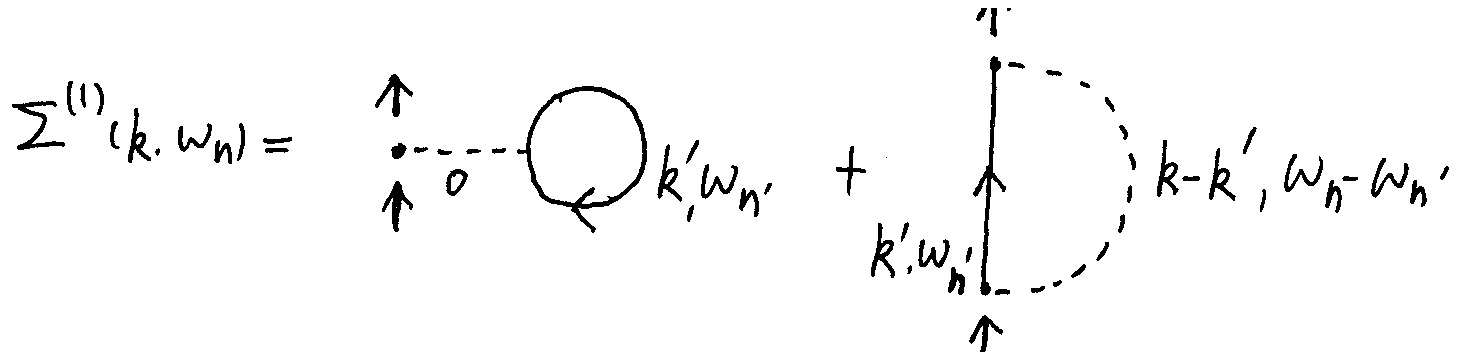
\includegraphics[width=10cm]{1stselfenergy.png}
\caption{一阶自能图}
%\label{default}
\end{center}
\end{figure}


写出$\Sigma^{(1)}(k, \omega_n)$

\begin{equation}
 - \frac{1}{\beta} \sum\limits_{n'} e^{i \omega_{n'} \eta} \int  \frac{d^3 k'} {(2 \pi)^3} \mathcal{G}^0 (k', \omega_{n'}) \left[ -(2s+1) V(0) + V(k - k')  \right]
\end{equation}

改写为:

\begin{equation*}
\int \frac{d^3 k'}{(2 \pi)^3} \left[ (2s+1) V(0) - V(k-k') \right] \cdot \frac{1}{\beta} \sum\limits_{n'} \frac{e^{i \omega_{n'} \eta} }{ i \omega_{n'}  - \epsilon_{k'} + \mu }
\end{equation*}

现在需要计算频率求和:

\begin{equation}
\frac{1}{\beta} \sum\limits_n e^{i \omega_n \eta} (i \omega_n - x )^{-1}
\end{equation}

可以证明:

\begin{equation}
\sum\limits_n \frac{ e^{ i \omega_n \eta } }{ i \omega_n - x } = \mp \frac{\beta}{  e^{\beta x} \mp 1 }
\end{equation}

“-”是玻色子,“+”是费米子。

因此:

\begin{equation}
\Sigma^{(1)}(k) = \int \frac{d^3 k'}{(2 \pi)^3} \left[ (2s+1)V(0) - V(k - k') \right] n^0_{k'}
\end{equation}

这里,费米子的$n^0_{k'}$

\begin{equation}
n^0_{k'} = \frac{1}{ e^{ \beta ( \epsilon^0_{k'} - \mu  ) } + 1 }
\end{equation}

\subsection{频率求和}

\subsubsection{费米子的频率求和}

考虑费米子,$\omega_n = \frac{ (2n+1) \pi}{\beta}$,求证:

\begin{equation}
\sum\limits_{n \in odd } \frac{e^{i \omega_n \eta}}{i \omega_n - x } =\frac{ \beta}{ e^{\beta x} + 1 }
\end{equation}

证:

考虑复函数:

\begin{equation}
f(z) = \frac{1}{e^{\beta z} + 1}
\end{equation}

$f(z)$在复平面上奇点的位置:$\beta z = i (2n +1) \pi$,即:

\begin{equation*}
z = i \omega_n = \frac{i (2n +1)\pi }{\beta}
\end{equation*}

在这些奇点上$f(z)$的留数是:

\begin{equation*}
\lim\limits_{z \to i\omega_n  } \frac{z - i \omega_n}{ e^{\beta z} + 1 } =  \lim\limits_{z \to i\omega_n  } \frac{1}{ \beta e^{\beta z}  } = - \frac{1}{\beta}
\end{equation*}

这里利用了“罗比达”法则:$\lim\limits_{z \to z_0} \frac{f(z)}{g(z)} = \lim\limits_{z \to z_0} \frac{ f'(z) }{ g'(z) } $

\begin{figure}[htbp]
\begin{center}
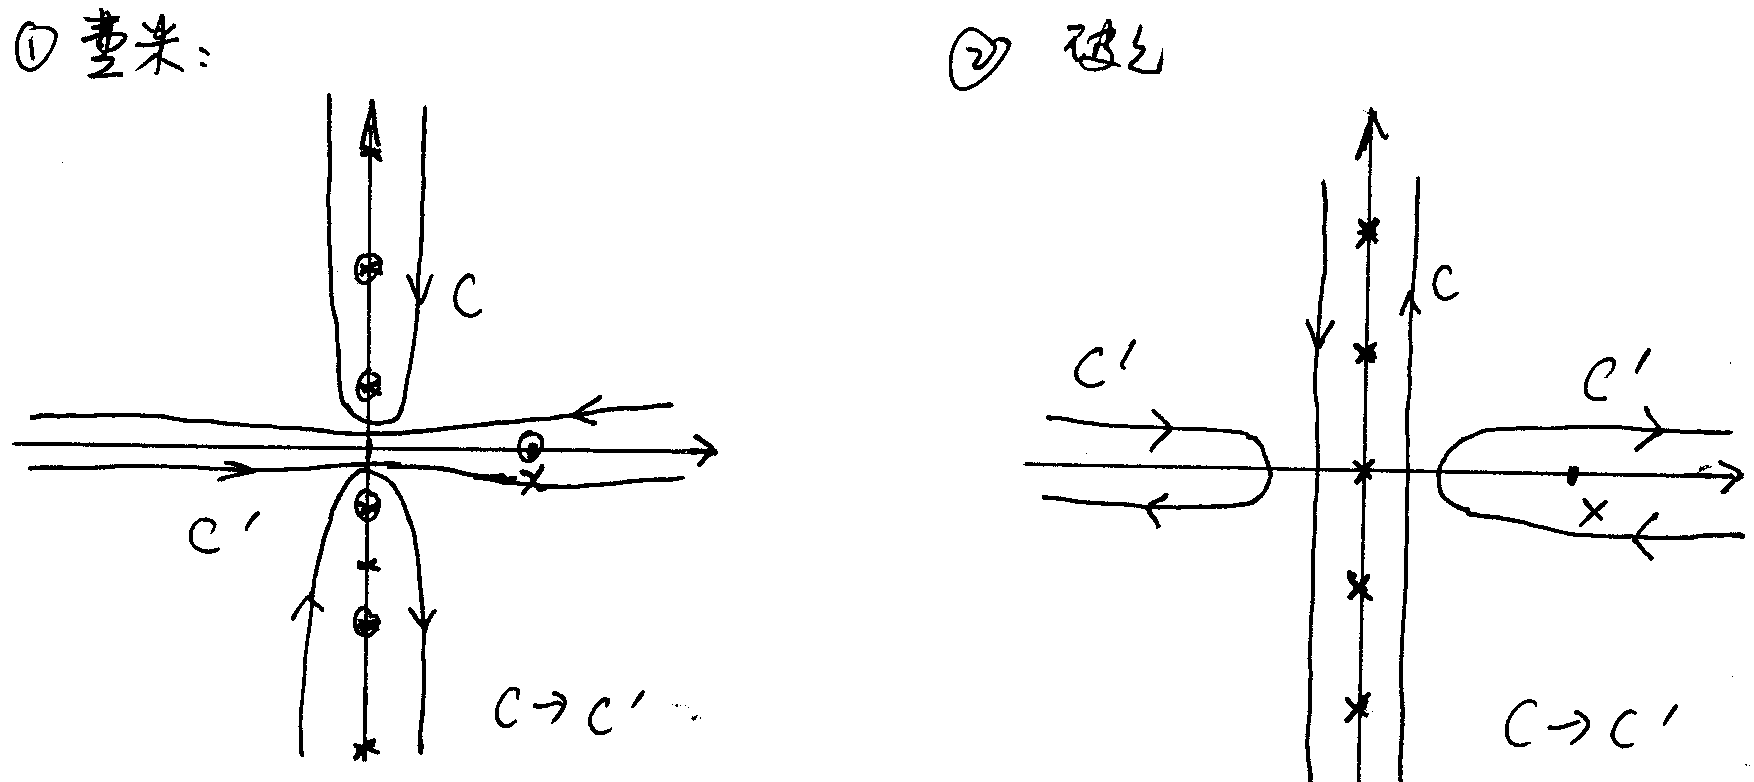
\includegraphics[width=10cm]{Finite/frequencysummation.png}
\caption{频率求和}
%\label{default}
\end{center}
\end{figure}

考虑积分:

\begin{equation*}
\frac{1}{2\pi i} \int_C \frac{ dz e^{z \eta} }{z -x} f(z)
\end{equation*}

这个积分的奇点有:(1)$z = x$,在实轴上;(2)$z = i \omega_n$,在虚轴上的奇数格点。

积分回路C是顺时针的,总体会有一个“-”,但会与留数$- \frac{ 1 }{\beta} ...$的“-”抵消。积分回路C'是逆时针的。

最终结果是:

\begin{equation}
\frac{1}{\beta} \sum\limits_n \frac{e^{i \omega_n \eta}}{ i \omega_n - x} = f(x) = \frac{1}{e^{\beta (\epsilon_k - \mu)} + 1 }
\end{equation}


\subsubsection{玻色子的频率求和}

考虑玻色子,$\omega_n = \frac{2n \pi}{\beta}$,求证:

\begin{equation}
\sum\limits_{n \in even} \frac{e^{i \omega_n \eta}}{i \omega_n - x } =\frac{- \beta}{ e^{\beta x} - 1 }
\end{equation}

证:

考虑复函数:

\begin{equation}
f_B (z)  = \frac{1}{e^{\beta z}  -1}
\end{equation}

奇点位置$z = i \omega_n$,$\omega_n = \frac{2n \pi}{ \beta}$

$f_B(z)$在$i \omega_n$处的留数:

\begin{equation*}
\lim\limits_{z \to i \omega_n}  \frac{z - i \omega_n}{ e^{\beta z }  - 1 } = \frac{(...)'}{(...)'} = \frac{1}{\beta}
\end{equation*}

构造积分:

\begin{equation}
\frac{1}{2 \pi i } \int_C \frac{dz e^{z \eta}} { z -x }
\end{equation}

积分回路C是逆时针的;积分回路C'是顺时针的,因此有一个额外的“-”。

因此:

\begin{equation*}
\frac{1}{\beta} \sum\limits_n \frac{ e^{i \omega_n \eta} } { i \omega_n - x } = - f_B (x) = - \frac{1}{e^{ \beta(\epsilon_k - \mu )} -1 }
\end{equation*}


\section{有限温度的时间格林函数}

\subsection{推广的莱曼表示}

首先拷贝热力学格林函数的定义, $t_1 > t_2$时,

\begin{eqnarray*}
% \nonumber to remove numbering (before each equation)
  iG_{\alpha \beta} (x_1 t_1, x_2 t_2) &=& Tr \left\{ e^{\beta \Omega}
e^{-\beta K } \psi_\alpha (x_1 t_1) \psi_\beta^\dagger (x_2
t_2) \right\} \\
  {} &=& \left\langle \psi_\alpha (x_1 t_1)
\psi_\beta^\dagger (x_2 t_2) \right\rangle
\end{eqnarray*}

其中, $K = H - \mu N$

\begin{eqnarray*}
% \nonumber to remove numbering (before each equation)
  \psi_\alpha(x_1 t_1) &=& e^{iK t_1} e^{-i P x_1} \psi_\alpha e^{i P x_1} e^{-i K t_1 } \\
  \psi^{\dagger}_{\beta} (x_2 t_2) &=& e^{i K t_2} e^{-i P x_2} \psi^{\dagger}_{\beta} e^{i P x_2} e^{-i K t_2 }
\end{eqnarray*}


假设系统是空间均匀的, $P$, $H$, $N$两两对易, 有共同本征态,
记作$\left| n \right\rangle$, 本征值分别为$P_n$, $E_n$, 和$N_n$ (或
$K_n = E_n - \mu N_n$).

求Trace运算就是$\sum_n \left\langle n \right| \rho A \left| n
\right\rangle $,

\begin{equation*}
iG(1,2) = \sum_{nm} \left\langle n \right| \rho \psi(1) \left| m
\right\rangle \left\langle m \right| \psi^\dagger(2) \left| n
\right\rangle
\end{equation*}

这里,

\begin{eqnarray*}
% \nonumber to remove numbering (before each equation)
  \left\langle n \right| \rho \psi(1) \left| m \right\rangle &=& e^{\beta \Omega} e^{-\beta K_n} e^{i K_n t_1} e^{-i P_n x_1}
e^{i P_m x_1} e^{- i K_m t_1}  \left\langle n \right| \psi_\alpha
\left| m \right\rangle \\
  {} &=& e^{\beta \Omega} e^{-\beta K_n} e^{- i(K_m - K_n) t_1} e^{i (P_m
- P_n) x_1} \left\langle n \right| \psi_\alpha \left| m
\right\rangle
\end{eqnarray*}

类似地,

\begin{eqnarray*}
% \nonumber to remove numbering (before each equation)
  \left\langle m \right| \psi^\dagger(2) \left| n \right\rangle &=& e^{iK_m t_2} e^{-i P_m x_2} e^{i P_n x_2} e^{-i K_n t_2}
\left\langle m \right| \psi_\beta^\dagger \left| n \right\rangle \\
  {} &=& e^{i(K_m - K_n) t_2} e^{-i (P_m - P_n) x_2 } \left\langle m
\right| \psi_\beta^\dagger \left| n \right\rangle
\end{eqnarray*}


令:

\begin{eqnarray*}
% \nonumber to remove numbering (before each equation)
  P_{mn} &=& P_m - P_n \\
  \omega_{mn} &=& K_m - K_n
\end{eqnarray*}


$iG(1,2)$, $t_1 > t_2$可表示为:


\begin{equation*}
iG(1,2) = e^{\beta \Omega} \sum_{nm} e^{-\beta K_n} e^{iP_{mn}(x_1 -
x_2)} e^{-i\omega_{mn} (t_1 - t_2)} \left\langle n \right|
\psi_\alpha \left| m \right\rangle \left\langle m \right|
\psi_\beta^\dagger \left| n \right\rangle
\end{equation*}

对$t_1 < t_2 $, 需要计算$Tr \left\{ \rho \psi_2^\dagger \psi_1
\right\} = \sum_{nm} \left\langle n \right| \rho \psi_2^\dagger
\left| m \right\rangle \left\langle m \right| \psi_1 \left| n
\right\rangle $, 与$t_1 > t_2$的展开比较, $Tr \left\{ \rho \psi_1
\psi_2^\dagger \right\} = \sum_{nm} \left\langle n \right| \rho
\psi_1 \left| m \right\rangle \left\langle m \right| \psi_2^\dagger
\left| n \right\rangle $. 对$t_1 < t_2$, 将求和指标$n,m$互换, 得到:

\begin{equation*}
Tr \left\{ \rho \psi_2^\dagger \psi_1 \right\} = \sum_{nm}
\left\langle m \right| \rho \psi_2^\dagger \left| n \right\rangle
\left\langle n \right| \psi_1 \left| m \right\rangle
\end{equation*}

由上式, 我们可直接写出$t_1 < t_2$时的$iG(1,2)$,


\begin{equation*}
iG(1,2) = \mp e^{\beta \Omega} \sum_{nm} e^{-\beta K_m}
e^{iP_{mn}(x_1 - x_2)} e^{-i \omega_{mn}(t_1 - t_2)} \left\langle n
\right| \psi_\alpha \left| m \right\rangle \left\langle m \right|
\psi_\beta^\dagger \left| n \right\rangle
\end{equation*}

现在令, $x=x_1 - x_2$, $t=t_1 - t_2$, 得到$iG_{\alpha
\beta}(xt)$的表达式, 让后将其变换到动量, 频率空间$iG_{\alpha
\beta}(p, \omega)$.

FT的定义式为:


\begin{equation*}
G(p, \omega) = \int d^3x dt e^{-ipx}e^{i \omega t} G(xt)
\end{equation*}


这里对$t$的积分, 会因$t>0$, $t<0$分成两部分,
利用如下积分关系\footnote{利用关系: $\frac{1}{\omega \pm i \eta } =
P \frac{1}{\omega} \mp i \pi \delta(\omega ) $}:

\begin{eqnarray*}
% \nonumber to remove numbering (before each equation)
  \int_0^{\infty} dt e^{i \omega t} &=& \frac{i}{\omega + i \eta} = \frac{i}{\omega} + \pi \delta(\omega) \\
  \int_{-\infty}^0 dt e^{i \omega t} &=& - \frac{i}{\omega - i \eta}
  = - \frac{i}{\omega} + \pi \delta (\omega)
\end{eqnarray*}

对$x$的积分, 需要用到关系:

\begin{equation*}
\delta(  \vec p- \vec P_{mn}) =\frac{1}{(2\pi)^3} \int d^3 x e^{-i
(\vec p - \vec P_{mn})\cdot \vec x}
\end{equation*}

求得,


\begin{eqnarray*}
% \nonumber to remove numbering (before each equation)
  G_{\alpha \beta} (p, \omega) &=& (2\pi)^3 e^{\beta \Omega} \sum_{nm}
\left\langle n \right| \psi_\alpha \left| m \right\rangle
\left\langle m \right| \psi_\beta^\dagger \left| n \right\rangle
\delta(p-P_{mn})  \\
{} & \times &   \left\{ \frac{e^{-\beta K_n}}{\omega - \omega_{mn} +
i \eta} \pm \frac{e^{-\beta K_m}}{\omega - \omega_{mn} - i \eta}
\right\}
\end{eqnarray*}

假设哈密顿量中不含自旋指标, 如$H = \left( {\begin{array}{*{20}c}
   {H{}_{ +  + }} & 0  \\
   0 & {H_{ -  - } }  \\
 \end{array} } \right)$, $H_{++} = H_{--}$, $G_{\alpha \beta}(p, \omega) = \delta_{\alpha \beta} G(p,
 \omega)$, 于是:

 \begin{equation*}
 G(p,\omega) = \frac{1}{2S+1} G_{\alpha \alpha} (p, \omega)
 \end{equation*}

这里的$G_{\alpha \alpha}$要对自旋指标$\alpha$求和,

\begin{eqnarray*}
% \nonumber to remove numbering (before each equation)
G_{\alpha \alpha} (p, \omega) &=& (2\pi)^3 e^{\beta \Omega} \sum_{nm,\alpha} | \left\langle n \right| \psi_\alpha \left| m \right\rangle  |^2 \delta(p-P_{mn}) e^{-\beta K_n}    \\
  {} & \times & \left\{ P \frac{1}{\omega - \omega_{mn}} [1 \pm e^{-\beta \omega_{mn}}] - i \pi \delta(\omega - \omega_{mn}) [1 \mp e^{-\beta \omega_{mn}}] \right\}
\end{eqnarray*}

现在来讨论格林函数$G(p, \omega)$虚部与实部之间的关系,

首先$\omega_{mn} \to \omega'$,

\begin{eqnarray*}
% \nonumber to remove numbering (before each equation)
  G(p, \omega) &=& \sum_{nm, \alpha} ... \\
  {} &=& \int d \omega' ...\left\{ P
\frac{1}{\omega - \omega'} [1 \pm e^{-\beta \omega'}] - i \pi
\delta(\omega - \omega') [1 \mp e^{-\beta \omega'}] \right\}
\end{eqnarray*}

由上式, 可推出关系:

\begin{equation*}
Re G(p, \omega) = \frac{P}{\pi} \int_{-\infty}^{\infty} d\omega'
\left[ \tanh \frac{\beta \omega'}{2} \right]^{\mp 1} \frac{Im G(p,
\omega')}{\omega' - \omega}
\end{equation*}


``$-$''对应费米子, ``$+$''对应玻色子。

现在引入超前和推迟热力学格林函数, $G^R$, $G^A$,
分别在上下半平面得到解析函数,

\begin{eqnarray*}
% \nonumber to remove numbering (before each equation)
iG^R(1,2) &=& \theta(t_1 - t_2) Tr \left\{ \rho [\psi(1), \psi^\dagger(2)]_{\pm} \right\} \\
iG^A(1,2) &=& - \theta(t_2 - t_2) Tr \left\{ \rho [\psi(1),
\psi^\dagger(2)]_{\pm} \right\}
\end{eqnarray*}

变换到动量, 频率空间,

\begin{eqnarray*}
% \nonumber to remove numbering (before each equation)
G^R (p, \omega) &=& \frac{(2\pi)^3}{2S+1} e^{\beta
\Omega}\sum_{nm,\alpha} e^{-\beta (E_n - \mu N_n)}
\left|\psi_{nm,\alpha} \right|^2 \delta(p-P_{mn}) \\
{} & \times & \left\{ \frac{1}{\omega - \omega_{mn}} -i \pi \delta(\omega -\omega_{mn}) (1 \pm e^{-\beta \omega_{mn}}) \right\}  \\
G^A(p, \omega) &=& \frac{(2\pi)^3}{2S+1} e^{\beta
\Omega}\sum_{nm,\alpha} e^{-\beta (E_n - \mu N_n)}
\left|\psi_{nm,\alpha} \right|^2 \delta(p-P_{mn}) \\
{} & \times &  \left\{ \frac{1}{\omega - \omega_{mn}} + i \pi
\delta(\omega -\omega_{mn}) (1 \pm e^{-\beta \omega_{mn}}) \right\}
\end{eqnarray*}


可证明,

\begin{equation*}
Re G^{R,A}(p, \omega) = \frac{P}{\pi} \int_{-\infty}^{\infty}
d\omega' \frac{Im G^{R,A} (p, \omega')}{ \omega' - \omega}
\end{equation*}

通过恰当地定义谱函数$\rho(p, \omega) = \sum_{nm,\alpha}...$,
我们把$G^{R,A}$改写为:

\begin{eqnarray*}
% \nonumber to remove numbering (before each equation)
  G^R (p, \omega) &=& \int_{-\infty}^{\infty} \frac{d\omega'}{2 \pi} \frac{\rho(p, \omega')}{\omega - \omega' + i\eta } \\
  G^A (p, \omega) &=& \int_{-\infty}^{\infty} \frac{d\omega'}{2 \pi} \frac{\rho(p, \omega')}{\omega - \omega' - i\eta }
\end{eqnarray*}

可见$G^{R,A}$分别在上、下半平面解析。


\subsection{求和规则}

我们可以证明, 对态密度$\rho(p, \omega)$, 满足如下求和规则(sum rule):

\begin{equation}\label{sum rule}
\int_{-\infty}^{\infty} \frac{d \omega}{2 \pi} \rho(p, \omega) = 1
\end{equation}

证:首先构造如下积分,

\begin{equation*}
I = \int_{-\infty}^{\infty} \frac{d \omega}{2 \pi} i G^R(p, \omega)
e^{-i \omega \eta} = i \int_{-\infty}^{\infty}
\int_{-\infty}^{\infty} \frac{d \omega d \omega'}{(2\pi)^2}
\frac{\rho(p, \omega') e^{-i\omega \eta}}{\omega - \omega' + i \eta}
\end{equation*}

我们先计算上式中对$d \omega$的积分, 这里需构造积分回路如图(\ref{sum
rule contour}).

\begin{equation*}
i \int_{-\infty}^{\infty}\frac{d\omega}{2\pi}\frac{e^{-i \omega
\eta}}{\omega - \omega' + i \eta} =1
\end{equation*}

\begin{figure}[h]
\begin{center}
  % Requires \usepackage{graphicx}
  \includegraphics[width=6cm]{Finite/sum-rule-contour.ps}\\
  \caption{$e^{-i \omega \eta}$保证通过下半平面大圆的积分为零.}\label{sum rule contour}
\end{center}
\end{figure}

现在留下的就只是对$d\omega'$的积分,

\begin{equation*}
I = \int_{-\infty}^{\infty} \frac{d \omega'}{2 \pi} \rho (p,
\omega') = \int_{-\infty}^{\infty}\frac{d \omega}{2 \pi} i G^R (p,
\omega) e^{-i \omega \eta}
\end{equation*}

考虑上式中对$d \omega$ 的积分,

\begin{equation*}
I = \int_{-\infty}^{\infty}\frac{d \omega}{2 \pi} i G^R (p, \omega)
e^{-i \omega \eta} = i G^R(p, \eta)=  \int d^3 x e^{-i px} i G^R (x,
\eta)
\end{equation*}

上式中的$iG^R(x, \eta)$是,

\begin{equation*}
i G^R (x, \eta) = \frac{i}{2S+1} \sum_{\alpha} G_{\alpha
\alpha}^R(x, \eta) = \frac{1}{2S+1} Tr \left\{\rho_G [\psi_\alpha
(x, \eta), \psi_\alpha^\dagger (0,0)]_{\pm} \right\}
\end{equation*}

由于$\eta \to 0^+$, $\psi_\alpha(x,\eta) \to \psi_\alpha(x,0)$,
现在, 上式中的求迹运算为,

\begin{equation*}
Tr \left\{\rho_G [\psi_\alpha (x), \psi_\alpha^\dagger (0)]_{\pm}
\right\} = e^{\beta \Omega} \sum_{n, \alpha} e^{-\beta K_n}
\left\langle n \right| [\psi_\alpha (x), \psi_\alpha^\dagger
(0)]_{\pm} \left| n \right\rangle
\end{equation*}

场算符$\psi, \psi^\dagger$ 满足:

\begin{equation*}
[\psi_\alpha (x), \psi_\alpha^\dagger (0)]_{\pm} = \delta_{\alpha
\alpha} \delta (x)
\end{equation*}

因此,

\begin{equation*}
iG^R (x, \eta) =\frac{1}{2S+1} \sum_\alpha \left\{ \delta_{\alpha
\alpha} \delta(x) \right\} = \delta (x)
\end{equation*}

因此,

\begin{eqnarray*}
% \nonumber to remove numbering (before each equation)
  I &=& \int_{-\infty}^{\infty} \frac{d \omega}{2 \pi} \rho(p, \omega) \\
  & = & \int d^3 x e^{-i px} i G^R (x, \eta) = \int d^3 x e^{-i px} \delta(x) = 1
\end{eqnarray*}

\subsection{松原函数和解析延拓}

松原函数的定义是:

\begin{equation}
\mathcal{G} (x, \tau) = -\frac{1}{2s+1} Tr \{ e^{\beta \Omega} e^{- \beta K } \psi_{\alpha} (x,\tau) \psi_{\alpha}^\dagger (0)  \}  
\end{equation}

这里:$\psi_{\alpha}(x,\tau) = e^{-i P x } e^{K \tau} \psi_{\alpha}  e^{- K \tau} e^{i P x} $

类似先前的推导:

\begin{equation}
\mathcal{G}(x,\tau) = -\frac{ e^{\beta \Omega} }{2s+1} \sum\limits_{nm} e^{ - \beta K_n} e^{i P_{mn} x - \omega_{mn} \tau} \left| \left\langle n \right|  \psi_{\alpha} \left| m \right\rangle \right|^2 
\end{equation}

傅里叶变换,把宗量变为$p, i \omega$

\begin{eqnarray*}
\mathcal{G}(p, i \omega_l) &=& \int d^3 x \int_0^{\beta} d \tau e^{ -ipx + i \omega_l \tau } \mathcal{G} (x,\tau)    \\
{} &=& \frac{e^{\beta \Omega}}{ 2s+1 } \sum\limits_{nm} e^{-\beta K_n} (2\pi)^3 \delta(p - P_{mn}) \left| \left\langle n \right| \psi_{\alpha} \left| m \right\rangle  \right|^2 (1 \pm e^{-\beta \omega_{mn}} )\frac{1}{ i \omega_l - \omega_{mn}}
\end{eqnarray*}

这里由于$\tau$的取值是$ - \beta \to \beta$,$\omega_l$的取值是离散的,费米子位于奇数格点,而玻色子位于偶数格点。

利用谱函数$\rho (p, \omega)$的定义\footnote{蔡建华 \& 龚昌德:公式(3.6.19)},将$\mathcal{G} (p, i \omega_l )$改写为:

\begin{equation}
\mathcal{G}(p, i \omega_l) = \int_{-\infty}^{\infty} \frac{d \omega' }{2 \pi} \frac{\rho(p,\omega')}{ i \omega_l - \omega'}
\end{equation}

$\mathcal{G}(p, i \omega_l)$是个定义在分立点集$\{ i \omega_l  \}$上的复函数,我们将其延拓到整个复平面,定义复函数:

\begin{equation}
\Gamma (p, z) = \int_{-\infty}^{\infty} \frac{d \omega'}{2 \pi} \frac{\rho(p, \omega')}{z - \omega'} 
\end{equation}

$\Gamma(p,z)$与$G^R$,$G^A$,$\mathcal{G}$的关系是:

\begin{eqnarray}
G^R (p, \omega) &=& \Gamma (p, \omega + i \eta) \\
G^A (p, \omega) &=& \Gamma (p, \omega - i \eta) \\
\mathcal{G} (p, i \omega_l) &=& \Gamma (p, i \omega_l)
\end{eqnarray}

如果知道在分立点集$\{ i \omega_l \}$上的$\Gamma (p, z)$,需解析延拓到整个复$z$平面。这种解析延拓一般来说不是唯一的,假设$\Gamma (p,z)$是一个可能的延拓,对任意整数$p'$,函数$e^{2 \pi p' z / \omega_n} \Gamma(p,z) $是另一个可能的延拓。

利用求和规则(Sum Rule),当$\left| z \right| \to \infty$,$\Gamma (p, z) \to \frac{1}{z}$,我们能够挑选合适的解析延拓,并保证是唯一的\footnote{费特 \& 瓦里克:pp379;G. Baym \& N. D. Mermin,J. Math. Phys.,2:232(1961) }。

如果我们求出了$\mathcal{G}(p, i \omega_l) $,我们也就求出了$G^{R,A} (p, \omega)$

我们可以证明:

\begin{equation}
\rho(p, \omega) = i \left[ G^R (p, \omega) - G^A (p, \omega) \right]
\end{equation}

一般把$i \omega_l$形式上当作连续变量,直接从$\mathcal{G} (p, i \omega_l)$计算$\rho(p, \omega)$


\begin{equation}
\rho(p, \omega) = i \left[ \mathcal{G} (p, i \omega_l )|_{i \omega_l = \omega + i \eta}  - \mathcal{G} (p, i \omega_l )|_{i \omega_l = \omega - i \eta} \right]
\end{equation}

\subsection{态密度}

以费米子为例讨论态密度$N(\omega)$和热力学格林函数的关系。

定义:

\begin{eqnarray}
G_{\alpha \beta}^{>} (xt,x't') &=& -i Tr \{ e^{\beta (\Omega - K) }  \psi_{\alpha} (xt) \psi_{\beta}^{\dagger} (x't')   \} \\
G_{\alpha \beta}^{<} (xt,x't') &=& i Tr \{ e^{\beta ( \Omega - K) }   \psi_{\beta}^{\dagger} (x't') \psi_{\alpha} (xt)  \}
\end{eqnarray}

把场算符换到动量空间:

\begin{eqnarray}
\psi_{\alpha} (xt) &=& \frac{1}{\sqrt{V}} \sum\limits_p e^{i px} a_{p \alpha} (t) \\
\psi^{\dagger}_{\beta} (x't') &=& \frac{1}{\sqrt{V}} \sum\limits_p e^{ - i px' } a^{\dagger}_{p \beta} (t')
\end{eqnarray}

把上式代入$G_{\alpha \beta}^{>}$,$G_{\alpha \beta}^{<}$


\begin{eqnarray*}
G_{\alpha \beta}^{>} (xt,x't') &= & -\frac{i}{V} \sum\limits_{pp'} e^{ipx -ip'x'} \left\langle a_{p \alpha}(t)  a^{\dagger}_{p' \beta} (t') \right\rangle   \\
{}&=& -\frac{i}{V} \sum\limits_p e^{ip(x-x')} \left\langle a_{p \alpha}(t)  a^{\dagger}_{p \beta} (t') \right\rangle
\end{eqnarray*}

这里要利用反对易关系:$\{ a_p , a^{\dagger}_{p'}  \} = \delta (p - p') $

类似地,还有:

\begin{equation*}
G_{\alpha \beta}^{<} (xt,x't') = \frac{i }{V } \sum\limits_p e^{i p (x-x')} \left\langle a^{\dagger}_{p \beta} (t') a_{p \alpha} (t)   \right\rangle
\end{equation*}

由此可求出傅里叶变换系数$G^{>}(p,\omega)$:

\begin{eqnarray*}
G^{>}_{\alpha \beta} (p,\omega) &=& -i \int dt e^{i \omega ( t - t' )} \left\langle  a_{p \alpha}(t) a^{\dagger}_{p \beta} (t')   \right\rangle \\
{} & = & -i \int dt e^{i \omega t } \left\langle  a_{p \alpha}(t) a^{\dagger}_{p \beta} (0)   \right\rangle
\end{eqnarray*}

类似地,我们可求:

\begin{equation*}
G^{<}_{\alpha \beta} (p,\omega) = i \int dt e^{i \omega t} \left\langle a^{\dagger}_{p \beta} (0)  a_{p \alpha} (t)  \right\rangle
\end{equation*}

现在定义$N^{>} (\omega) $为由$m \to n$,使态$n$增加一个粒子而使其能量增加$\omega $可利用的空状态数。

\begin{equation}
N^{>} (\omega) = \frac{1}{V} \sum\limits_p \sum\limits_m \left| \left\langle m \right| a^{\dagger}_{p \alpha}  \left|  n  \right\rangle  \right|^2 \delta(E_m - E_n - \omega)
\end{equation}

在零温下,我们可以证明:

\begin{equation}
N^{>} (\omega) = \frac{1}{V} \sum\limits_p \int \frac{dt }{2 \pi } e^{i \omega t } \left\langle n \right|  a_{p \alpha} (t)  a^{\dagger}_{p \alpha} (0) \left| n  \right\rangle
\end{equation}

在有限温度下,对上式求统计平均:

\begin{equation}
N^{>} (\omega , T) = \frac{1}{V}  \sum\limits_p \int \frac{dt }{2 \pi } e^{i \omega t } \left\langle a_{p \alpha} (t) a^{\dagger}_{p \alpha } (0) \right\rangle
\end{equation}

$N^{>} (\omega, T)$的意义是:对一个处在热平衡态的系统,当增加一个粒子而使其能量增加$\omega $时可利用的空状态数。

类似地,我们可定义$N^{<} (\omega , T )$

\begin{equation}
N^{<} (\omega , T) = \frac{1}{V}  \sum\limits_p \int \frac{dt }{2 \pi } e^{i \omega t } \left\langle  a^{\dagger}_{p \alpha } (0)  a_{p \alpha} (t)  \right\rangle
\end{equation}

$N^{<} (\omega, T)$的意义是:对一个处在热平衡态的系统,当除去一个粒子而使其能量减少$\omega $时可利用的满状态数。($ n \to m$)

我们可以证明:

\begin{eqnarray}
N^{>} (\omega, T) &=& \frac{i}{2 \pi V } \sum\limits_p G^{>}_{\alpha \alpha} (p, \omega)  \\
N^{<} (\omega, T) &=& - \frac{i }{2 \pi V} \sum\limits_p G^{<}_{\alpha \alpha} (p, \omega) 
\end{eqnarray}

能量为$\omega $的单粒子态密度$N(\omega)$是空状态数和满状态数之和。

\begin{eqnarray*}
N(\omega ) & = & N^{>} (\omega, T ) + N^{<} (\omega, T ) \\
{} & = & \frac{i }{2 \pi V} \sum\limits_p \left[ G^{>}_{\alpha \alpha} (p, \omega) - G^{<}_{\alpha \alpha} (p, \omega) \right]
\end{eqnarray*}

利用谱函数$\rho(p, \omega) $的定义,我们可以把$G^{>} (p, \omega) = \frac{1}{2s+1} G_{\alpha \alpha}^{> } (p, \omega) $改写为:

\begin{eqnarray}
G^{>} (p, \omega) &=& - \frac{i \rho(p, \omega)}{1+ e^{- \beta \omega}  }  \\
G^{<} (p, \omega) &=& \frac{i \rho(p, \omega) }{1 + e^{\beta \omega}}
\end{eqnarray}

由此可得到$N(\omega)$与$\rho(p, \omega)$的关系:

\begin{equation}
N(\omega) = \frac{2s + 1}{2 \pi V } \sum\limits_p \rho(p, \omega)
\end{equation}

根据$\rho = i \left[ G^R - G^A \right]$,$G^R - G^A \propto \Im G^{R/A}$,现在$N(\omega )$可表示为:

\begin{equation}
N(\omega ) = - \frac{1}{\pi V} \sum\limits_p \Im G_{\alpha \alpha}^R (p, \omega) = \frac{1}{\pi V} \sum\limits_p \Im G^A_{\alpha \alpha} (p, \omega)
\end{equation}

或改写为积分的形式:

\begin{eqnarray*}
N(\omega ) & = & -\frac{1}{\pi} \int \frac{d^3 p}{(2 \pi)^3 } \Im G^R_{\alpha \alpha} (p, \omega) \\
{} & = & \frac{1 }{\pi } \int \frac{d^3 p}{(2 \pi)^3 } \Im G^A_{\alpha \alpha} (p, \omega)
\end{eqnarray*}

也可写作松原函数的形式:

\begin{equation}
N(\omega ) = - \frac{1}{\pi } \int \frac{d^3 p}{(2 \pi)^3 } \Im \mathcal{G}_{\alpha \alpha} (p, \omega + i \eta)
\end{equation}

最后我们可以把热力学格林函数$G^{<}$表示为谱函数的形式:

\begin{eqnarray*}
G^{<} (p, t-t' )  &=& \int \frac{d \omega }{2 \pi} e^{ - i \omega (t - t' )} G^{<} (p, \omega  ) \\
{} &=& \int \frac{d \omega }{2 \pi} e^{ - i \omega ( t - t' ) } i \rho(p, \omega) f(\omega) 
\end{eqnarray*}

这里:

\begin{equation}
f(\omega ) = \frac{1}{1 + e^{\beta \omega}}
\end{equation}

类似地,

\begin{equation*}
G^{>} (p, t-t' )  =  \int \frac{d \omega }{2 \pi } e^{ - i \omega ( t - t' ) } (-i) \rho(p, \omega) f( - \omega) 
\end{equation*}



\subsection*{练习}

\begin{enumerate}

\item 

证明:对费米子:

\begin{equation}
\Re G (p, \omega) = \frac{\mathcal{P}}{\pi} \int_{- \infty}^{ \infty} d \omega' \coth \frac{\beta \omega'}{2} \frac{\Im G (p, \omega' )}{\omega' - \omega}
\end{equation}

证:

由$G (p, \omega)$ 出发:

\begin{eqnarray*}
G(p,\omega) = \frac{(2\pi)^3}{2s+1} e^{\beta \Omega} \sum\limits_{nm} e^{-\beta K_n } \left| \left\langle n \right| \psi \left| m \right\rangle  \right|^2 \delta(p - P_{mn}) \times \\
\{ \frac{\mathcal{P}}{\omega - \omega_{mn}} \left[ 1 \pm e^{-\beta \omega_{mn}} \right] - i \pi \delta (\omega - \omega_{mn}) \left[ 1 \mp e^{- \beta \omega_{mn}}  \right]   \}
\end{eqnarray*}

这里我们令$\omega_{mn} \to \omega'$


\begin{equation*}
\Im G(p, \omega') = ... \{ - \pi \delta(\omega - \omega' ) \left[ 1 \mp e^{- \beta \omega'} \right]  \}
\end{equation*}

格林函数的实部:

\begin{eqnarray*}
\Re G (p, \omega') &=& ... \{ \frac{\mathcal{P}}{ \omega - \omega' } \left[ 1 \pm e^{- \beta \omega' }  \right]   \} \\
{} &=& ...  \{ \frac{\mathcal{P}}{ \omega - \omega' } \left[ 1 \pm e^{- \beta \omega' }  \right]   \}\frac{ 1 \mp e^{- \beta \omega'} }{ 1 \mp e^{-\beta \omega'}  }
\end{eqnarray*}

上式两边同时乘以$ - \pi \delta(\omega - \omega' )$

\begin{eqnarray*}
- \pi \delta(\omega - \omega' ) \Re G(p, \omega' ) &=& ... \{ \frac{\mathcal{P}}{\omega - \omega'} \frac{1 \pm e^{- \beta \omega'}}{1 \mp e^{ - \beta \omega' } }  \} (1 \mp e^{ - \beta \omega' }) (- \pi \delta(\omega - \omega' ) )\\
{} &=& \frac{\mathcal{P}}{ \omega - \omega' } \frac{1 \pm e^{ - \beta \omega' } }{1 \mp e^{ - \beta \omega' } } \Im G(p, \omega')
\end{eqnarray*}

左右同时对$d \omega'$积分:

\begin{eqnarray*}
\Re G(p, \omega) &=& \int \delta (\omega - \omega' ) \Re G (p, \omega' ) \\
{}&=& \frac{1}{\pi} \int d \omega' \frac{1 \pm e^{-\beta \omega'}}{ 1 \mp e^{-\beta \omega'} } \frac{\mathcal{P}}{ \omega' - \omega} \Im G(p, \omega')
\end{eqnarray*}

对费米子而言:

\begin{equation*}
\frac{1+e^{-\beta \omega'}}{1- e^{-\beta \omega'} } = \frac{e^{\frac{\beta \omega'}{2}} + e^{-\frac{\beta \omega'}{2}}  }{ e^{\frac{\beta \omega'}{2}} - e^{-\frac{\beta \omega'}{2}}  } = \coth \frac{\beta \omega' }{2}
\end{equation*}

因此:

\begin{equation*}
\Re G (p, \omega) = \frac{\mathcal{P} }{\pi} \int_{- \infty}^{ \infty} d \omega' \coth \frac{\beta \omega'}{2} \frac{\Im G (p, \omega' )}{\omega' - \omega}
\end{equation*}

\item

请证明关系式:

\begin{equation*}
\rho(p, \omega) = i \left[ G^R (p, \omega) - G^A (p, \omega)  \right]
\end{equation*}

\end{enumerate}




\chapter{相互作用费米系}

\section{图形的部分求和}

\subsection{骨架图形}

高阶向前散射由于泡利不相容原理其贡献为零。

\begin{figure}[htbp]
\begin{center}
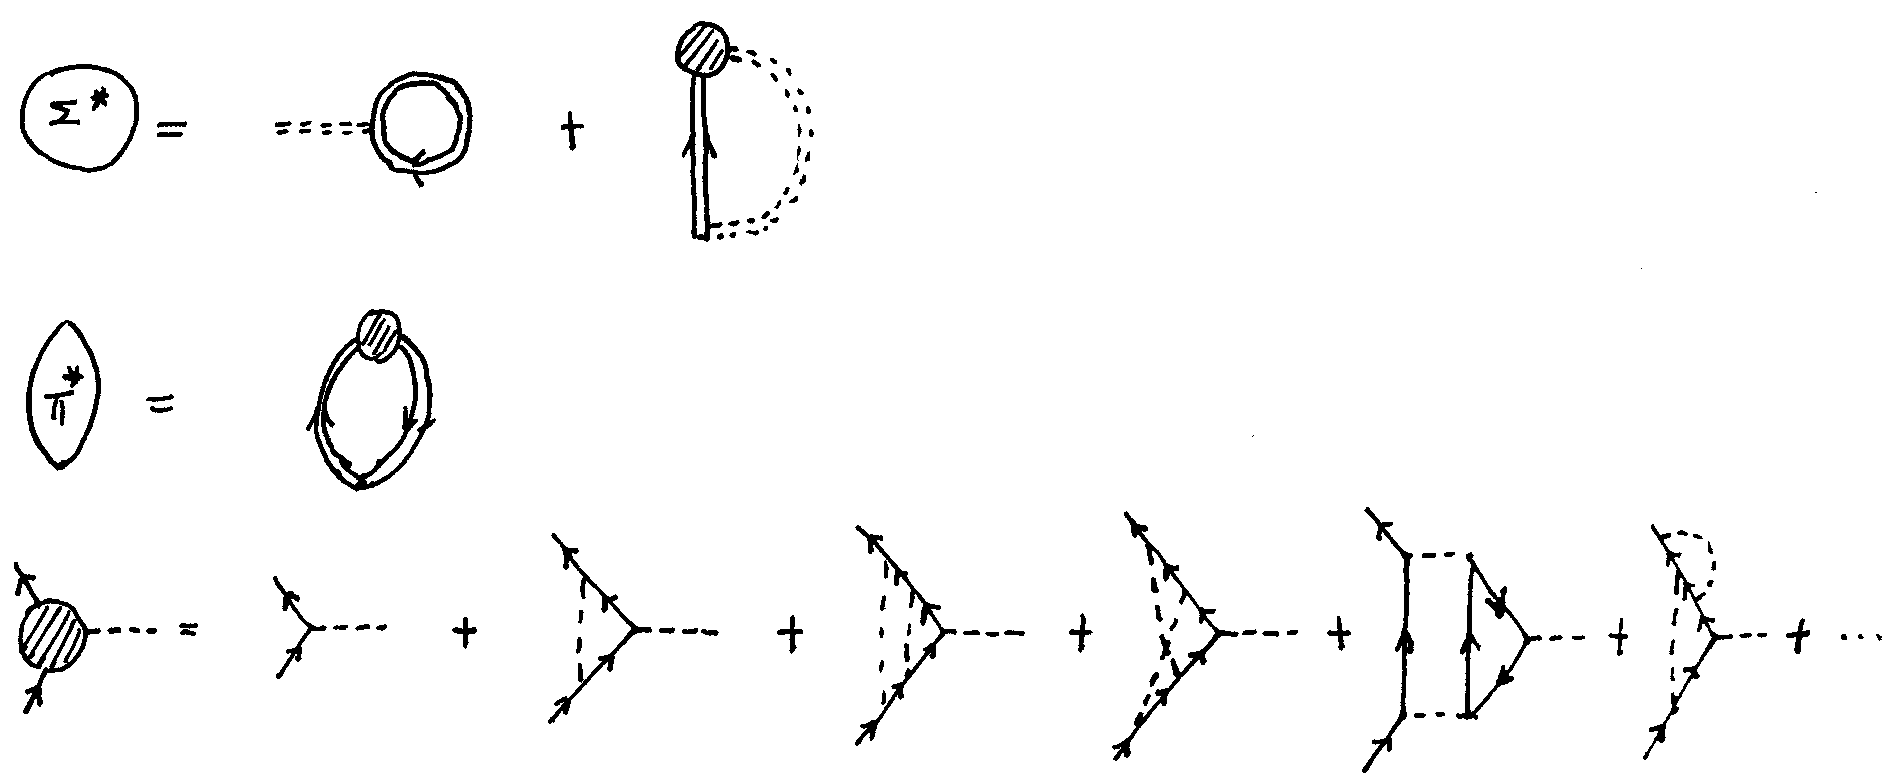
\includegraphics[width=11cm]{ManyF/skelepton.png}
%\caption{default}
%\label{default}
\end{center}
\end{figure}

正规顶角部分不能归结为有限个骨架图形的求和,这是我们无法完全精确地求出格林函数的原因。

定义双粒子格林函数:

\begin{equation}
G_2(12,34) = (-i)^2 \left\langle \Psi_H^0 \right| \mathcal{T} \{ \psi(1) \psi(2) \psi^\dagger (4) \psi^\dagger (3)  \} \left| \Psi_H^0  \right\rangle
\end{equation}

戈德斯通规定:

对于满费米球,湮灭掉一个费米球内($k < k_F $)的电子,$a_k \left| FS \right\rangle$,相对于真空态(FS)而言,能量为$- \epsilon(k)$,就是亏损了。用空穴激发(动量$-k$,能量$- \epsilon(k)$)描述多粒子系的这个态,$\epsilon^h = - \epsilon(k)$,空穴的波函数为:

\begin{equation}
\psi^h (t) = \phi(k) e^{-i (- \epsilon(k) ) t}
\end{equation}

这里可以有两种观点来看:

\begin{enumerate}
\item 

能量$\epsilon(k)$,时间$-t$,即一根逆着时间方向传播的粒子线;

\item

能量$- \epsilon(k)$,时间$t$,即一根顺着时间方向传播的粒子线;

\end{enumerate}

小结一下就是:逆着时间传播的粒子就是顺着时间传播的空穴。


%\begin{figure}[htbp]
%\begin{center}
%\includegraphics[width=15cm]{densityfluctuation.png}
%\caption{default}
%\label{default}
%\end{center}
%\end{figure}

\section{无规相近似}

\subsection{自洽的哈特利-福克近似}

只考虑自能修正($\Sigma^*$)而不考虑极化和顶角修正。

假设只计算到一阶图形:

\begin{equation}
\Sigma^*_{HF} = - 4 \pi e^2 \int_{k_1 < k_F} \frac{d^3 k_1 }{(2 \pi)^3 } \frac{1}{\left| k - k_1  \right|^2 }
\end{equation}

积分中$k$是常矢量,以$k$的方向为$z$轴建立球坐标系,$k_1$与$k$的夹角为$\theta$,

\begin{equation*}
d^3 k_1 = k_1^2 d k_1 \sin \theta d \theta d \phi
\end{equation*}

$\left|  k - k_1 \right|^2 = k^2 + k_1^2 - 2 k k_1 \cos \theta  $

\begin{eqnarray*}
\Sigma^*(k) & = & - \frac{4 \pi e^2 }{(2 \pi)^3 } \int_{k_1 < k_F} \frac{d^3 k_1}{ \left| k - k_1  \right|^2 }   \\
{}& = & - \frac{4 \pi e^2 }{(2 \pi)^3 } \int_0^{2 \pi}  \int_0^{\pi}  \int_0^{k_F} \frac{k_1^2 d k_1 \sin \theta d \theta d \phi }{ k^2 + k_1^2 - 2 k k_1 \cos \theta  } \\
{} &=& - \frac{e^2}{\pi} \int_0^{k_F} d k_1 \int_0^{\pi} \frac{k_1^2 \sin \theta d \theta }{k^2 + k_1^2 -2 k k_1 \cos \theta}
\end{eqnarray*}

变量变换:$t = \cos \theta$,$\sin \theta d \theta = - d \cos \theta$

\begin{equation*}
I = \int_0^{\pi} \frac{ k_1^2 \sin \theta d \theta  }{ k^2 + k_1^2 - 2 k k_1 \cos \theta } = \int_{-1}^{1}  \frac{k_1^2 d t }{ k^2 + k_1^2 - 2 k k_1 t  } 
\end{equation*}

变量变换:$\alpha = \frac{k }{k_1 }$

\begin{equation*}
I = \int_{-1}^1 \frac{dt}{\alpha^2 + 1 - 2 \alpha t  } = - \int_{-1}^1 \frac{d t }{2 \alpha t - (1 + \alpha^2 )  }
\end{equation*}

变量变换:$ t' = 2 \alpha t $,$d t' = 2 \alpha d t$

\begin{eqnarray*}
I &=& - \frac{1}{2 \alpha} \int_{ - 2 \alpha}^{ 2 \alpha }  \frac{ dt' }{ t' - (1 + \alpha)^2  } = - \frac{1}{2 \alpha} \left[ \ln  t'' \right]_{ - 2 \alpha - ( 1 + \alpha^2 )}^{ 2 \alpha - (1 + \alpha^2) } \\
{} & = & - \frac{1}{2 \alpha} \ln \frac{ 2 \alpha - (1 + \alpha)^2 }{ - 2 \alpha - (1 + \alpha^2 )  } = - \frac{1}{2 \alpha} \ln \frac{ \alpha^2 - 2 \alpha +1 }{ \alpha^2 + 2 \alpha +1 } \\
{} &=& - \frac{1}{\alpha} \ln \left| \frac{\alpha -1}{\alpha +1 }  \right| \\
{} &=& - \frac{k_1}{k} \ln \left| \frac{k - k_1}{ k + k_1 }  \right|
\end{eqnarray*}

现在要计算积分:

\begin{equation*}
\Sigma^*_{HF}(k ) = \frac{e^2 }{\pi}  \int_0^{k_F}  d k_1 \frac{k_1}{k} \ln \left|  \frac{ k - k_1 }{ k + k_1 } \right| 
\end{equation*}

变量变换:$ x = \frac{k_1}{ k } $, $k d x = d k_1$


\begin{equation*}
\Sigma^* = \frac{e^2 k}{\pi} \int_0^{k_F / k} x dx \ln \left| \frac{1-x}{1+x}  \right| = \frac{e^2 k}{\pi} \int_0^{k_F / k} x dx \left( \ln |1-x| - \ln |1+x|  \right)
\end{equation*}

分别考虑:

\begin{eqnarray*}
I_1 & = & \int_0^{k_F / k} x d x \ln | 1 - x |  \\
I_2 & = & \int_0^{k_F / k} x dx \ln | 1 + x |
\end{eqnarray*}

\begin{eqnarray*}
I_1 &=& \int_0^{k_F / k} \ln | 1- x | d\left( \frac{x^2}{2} \right) \\
{}&=& \left[ \frac{ x^2 \ln |1 -x| }{2} \right]_0^{k_F / k} - \int_0^{k_F / k}  \frac{x^2}{2} d \left( \ln | 1- x  | \right) \\
{} & = &  \frac{  \left( \frac{k_F}{k} \right)^2 \ln \left| 1 - \frac{ k_F }{ k } \right| }{2} - \frac{1}{2} \int_0^{k_F / k} \frac{x^2 d x}{x-1}
\end{eqnarray*}

类似地:

\begin{equation*}
I_2 = \frac{  \left( \frac{k_F}{k} \right)^2 \ln \left| 1 + \frac{ k_F }{ k } \right| }{2} - \frac{1}{2} \int_0^{k_F / k} \frac{x^2 d x}{x + 1}
\end{equation*}

\begin{equation*}
I_1 - I_2 = \frac{1}{2} \left( \frac{k_F}{k} \right)^2 \ln  \left|  \frac{ k - k_F }{ k + k_F }  \right| - \int_0^{k_F / k} \frac{x^2 }{x^2 - 1} dx
\end{equation*}

定义积分$I_3$

\begin{eqnarray*}
I_3 & = & \int_0^{k_F / k} \frac{x^2 dx}{x^2 -1} = \int_0^{k_F / k} \left( 1 + \frac{1}{x^2 - 1} \right) dx  = [x]_0^{ k_F / k  } + \frac{1}{2} \left[  \ln \left|  \frac{x-1}{x+1}   \right|  \right]_0^{k_F / k} \\
{} & = & \frac{k_F}{k } + \frac{1}{2} \ln \left| \frac{k_F - k}{k_F + k}  \right|
\end{eqnarray*}

因此:

\begin{equation*}
I_1 - I_2 = \frac{1}{2} \left(  \frac{k_F^2 - k^2}{ k^2 } \ln \left| \frac{ k-k_F }{k + k_F}  \right| \right) - \frac{k_F}{k}
\end{equation*}

代入得到HF近似下的自能:

\begin{eqnarray*}
\Sigma^*_{HF} (k) & =& \frac{e^2 k_F }{ 2 \pi } \left(  \left( \frac{k_F^2 - k^2}{ k k_F}  \right)  \ln \left| \frac{ k - k_F}{ k + k_F  } \right| - 2  \right) \\
{} & = & - \frac{e^2 k_F}{ 2 \pi } \left[ \frac{k_F^2 - k^2}{ k k_F } \ln \left| \frac{k_F + k}{ k_F - k }  \right|  + 2  \right] 
\end{eqnarray*}

\subsection*{阅读}

李正中,《固体理论》,第二版,第四章




%%%%%%%%%%

%\input{LehmannRepresentation}

%%%%%%%%%%

%\input{ensembles}

\end{document}